\chapter{RESULT \& ANALYSIS}
\section{Result}
 %The $S$ parameter simulation of single stage power amplifier(Figure \ref{fig:single-stage-power-amplifier}) is shown below
 \begin{figure}[H]
  \centering
  \begin{subfigure}{0.49\textwidth}
    \centering
    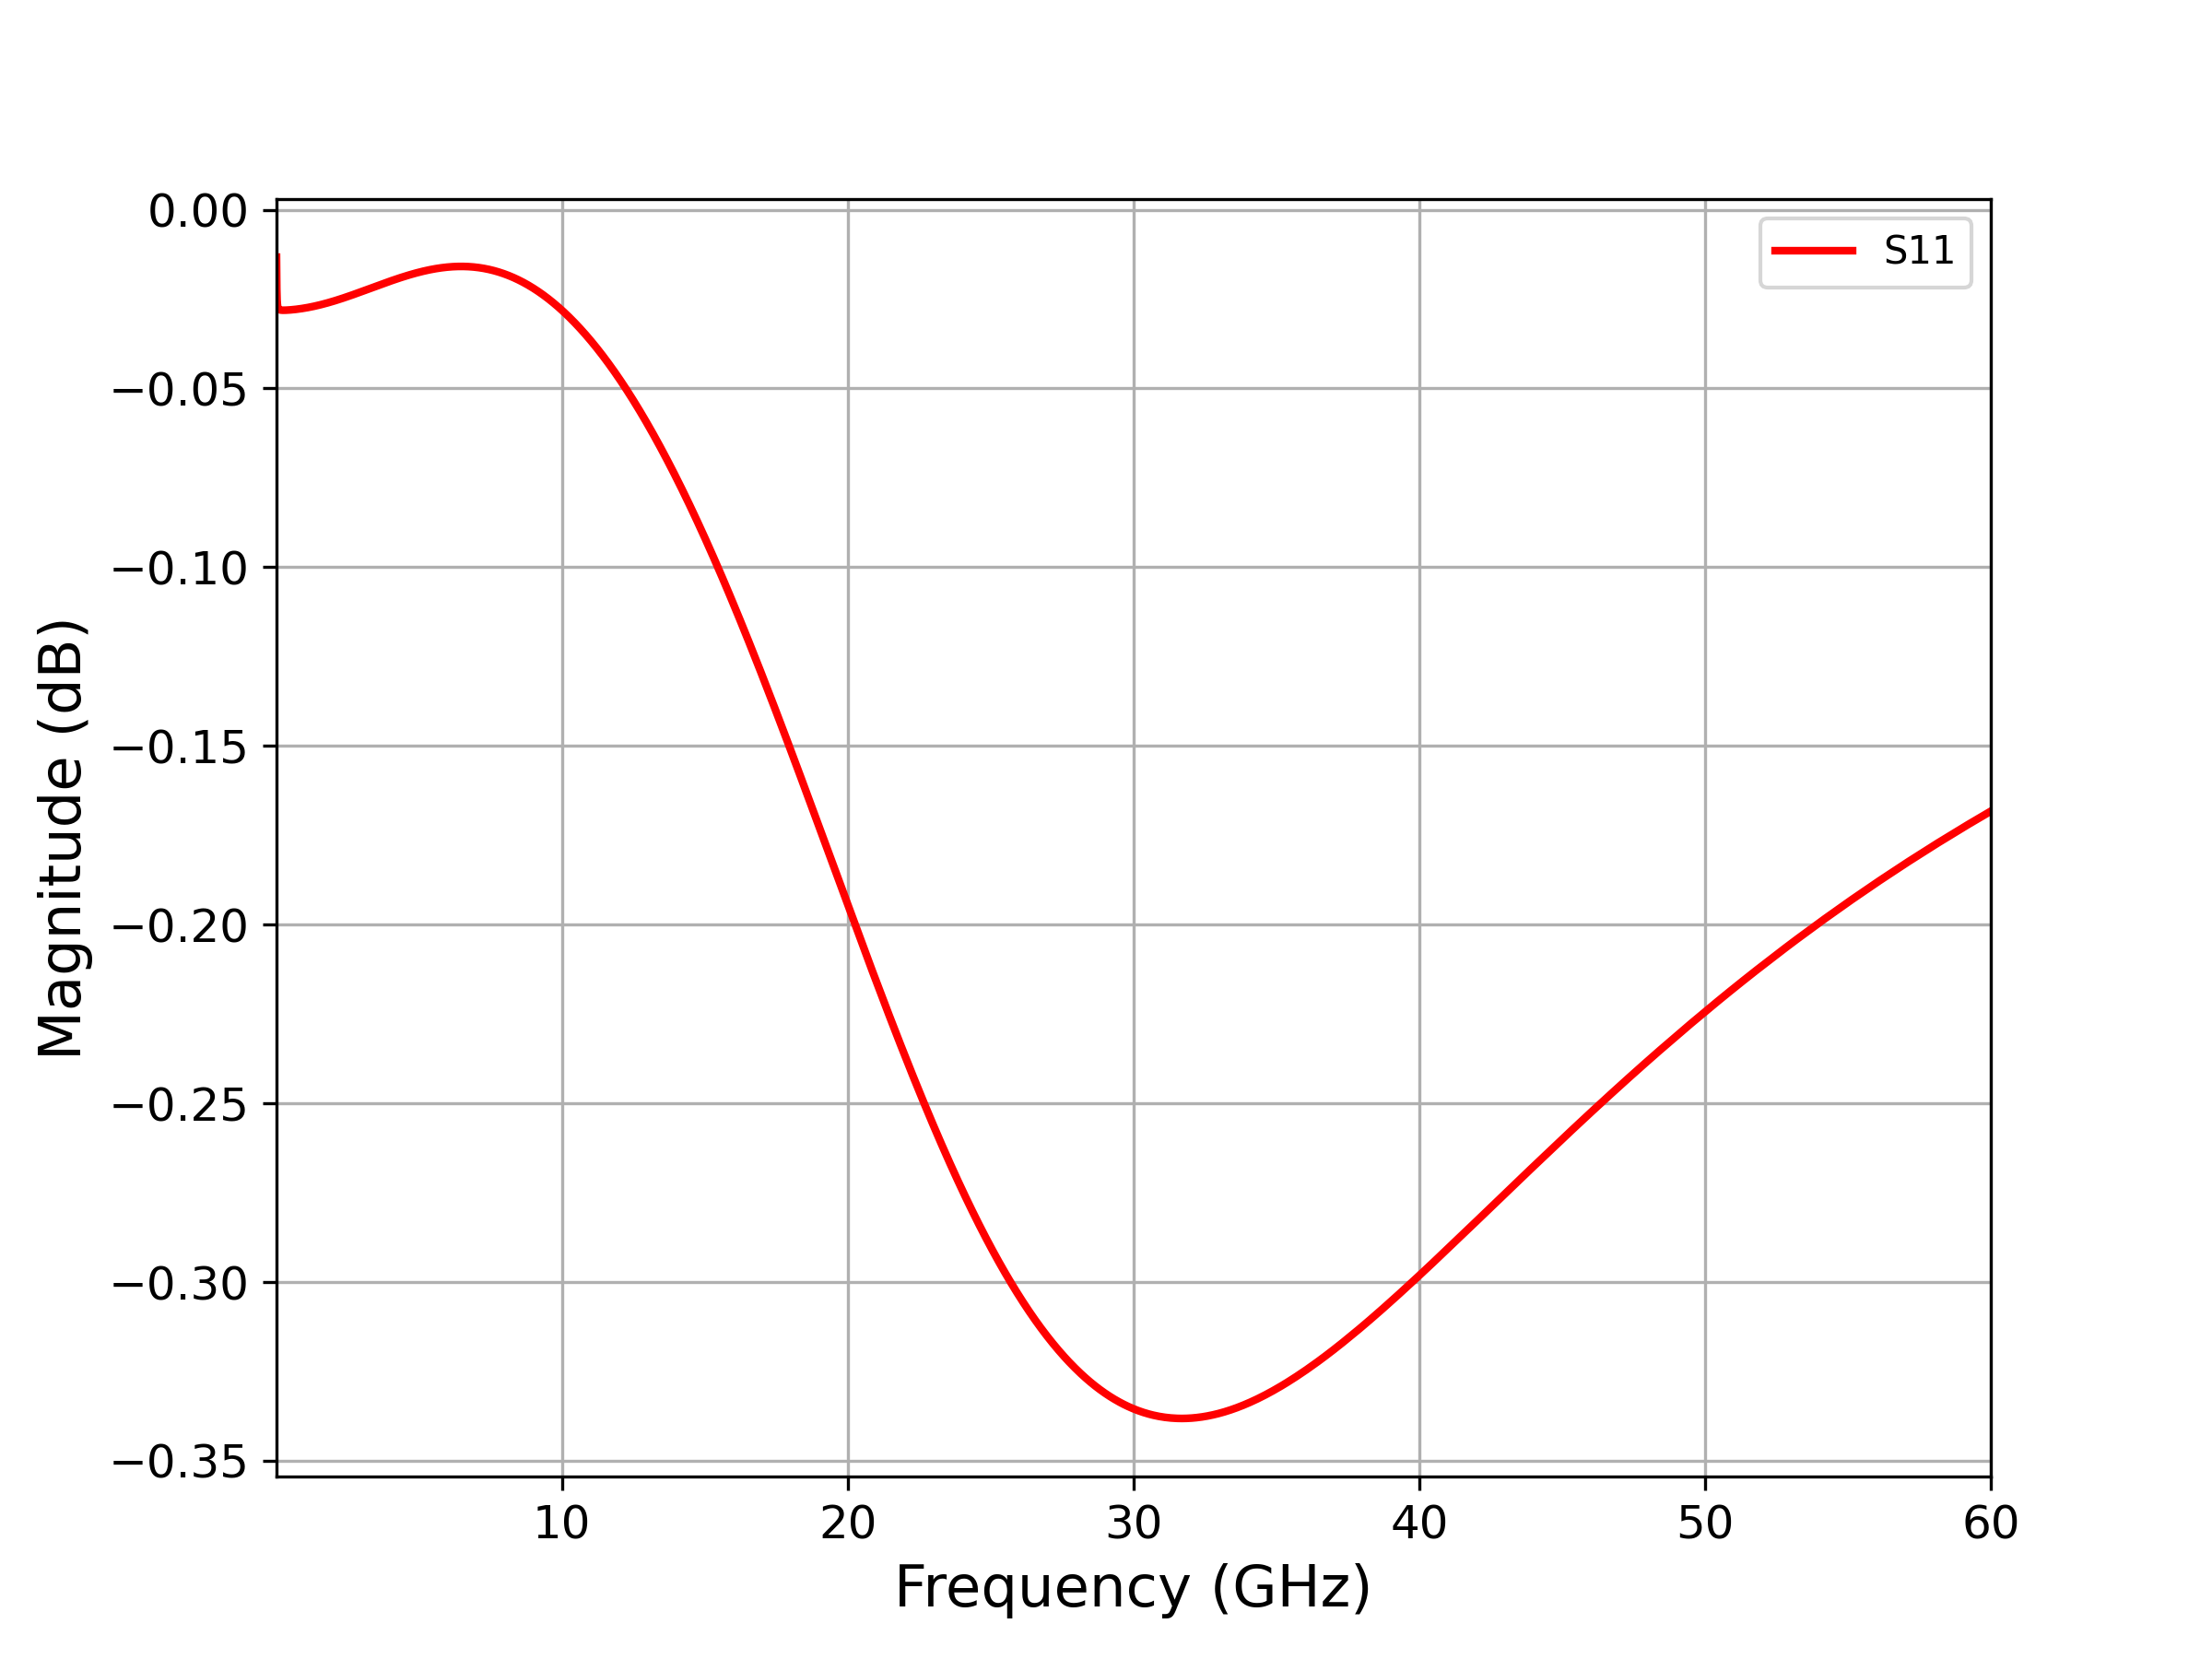
\includegraphics[width=\linewidth]{figures/single_stage_s11.png}
    \caption{}
    \label{fig:single-stage-without-cadence-s11}
  \end{subfigure}
  \hfill
  \begin{subfigure}{0.49\textwidth}
    \centering
    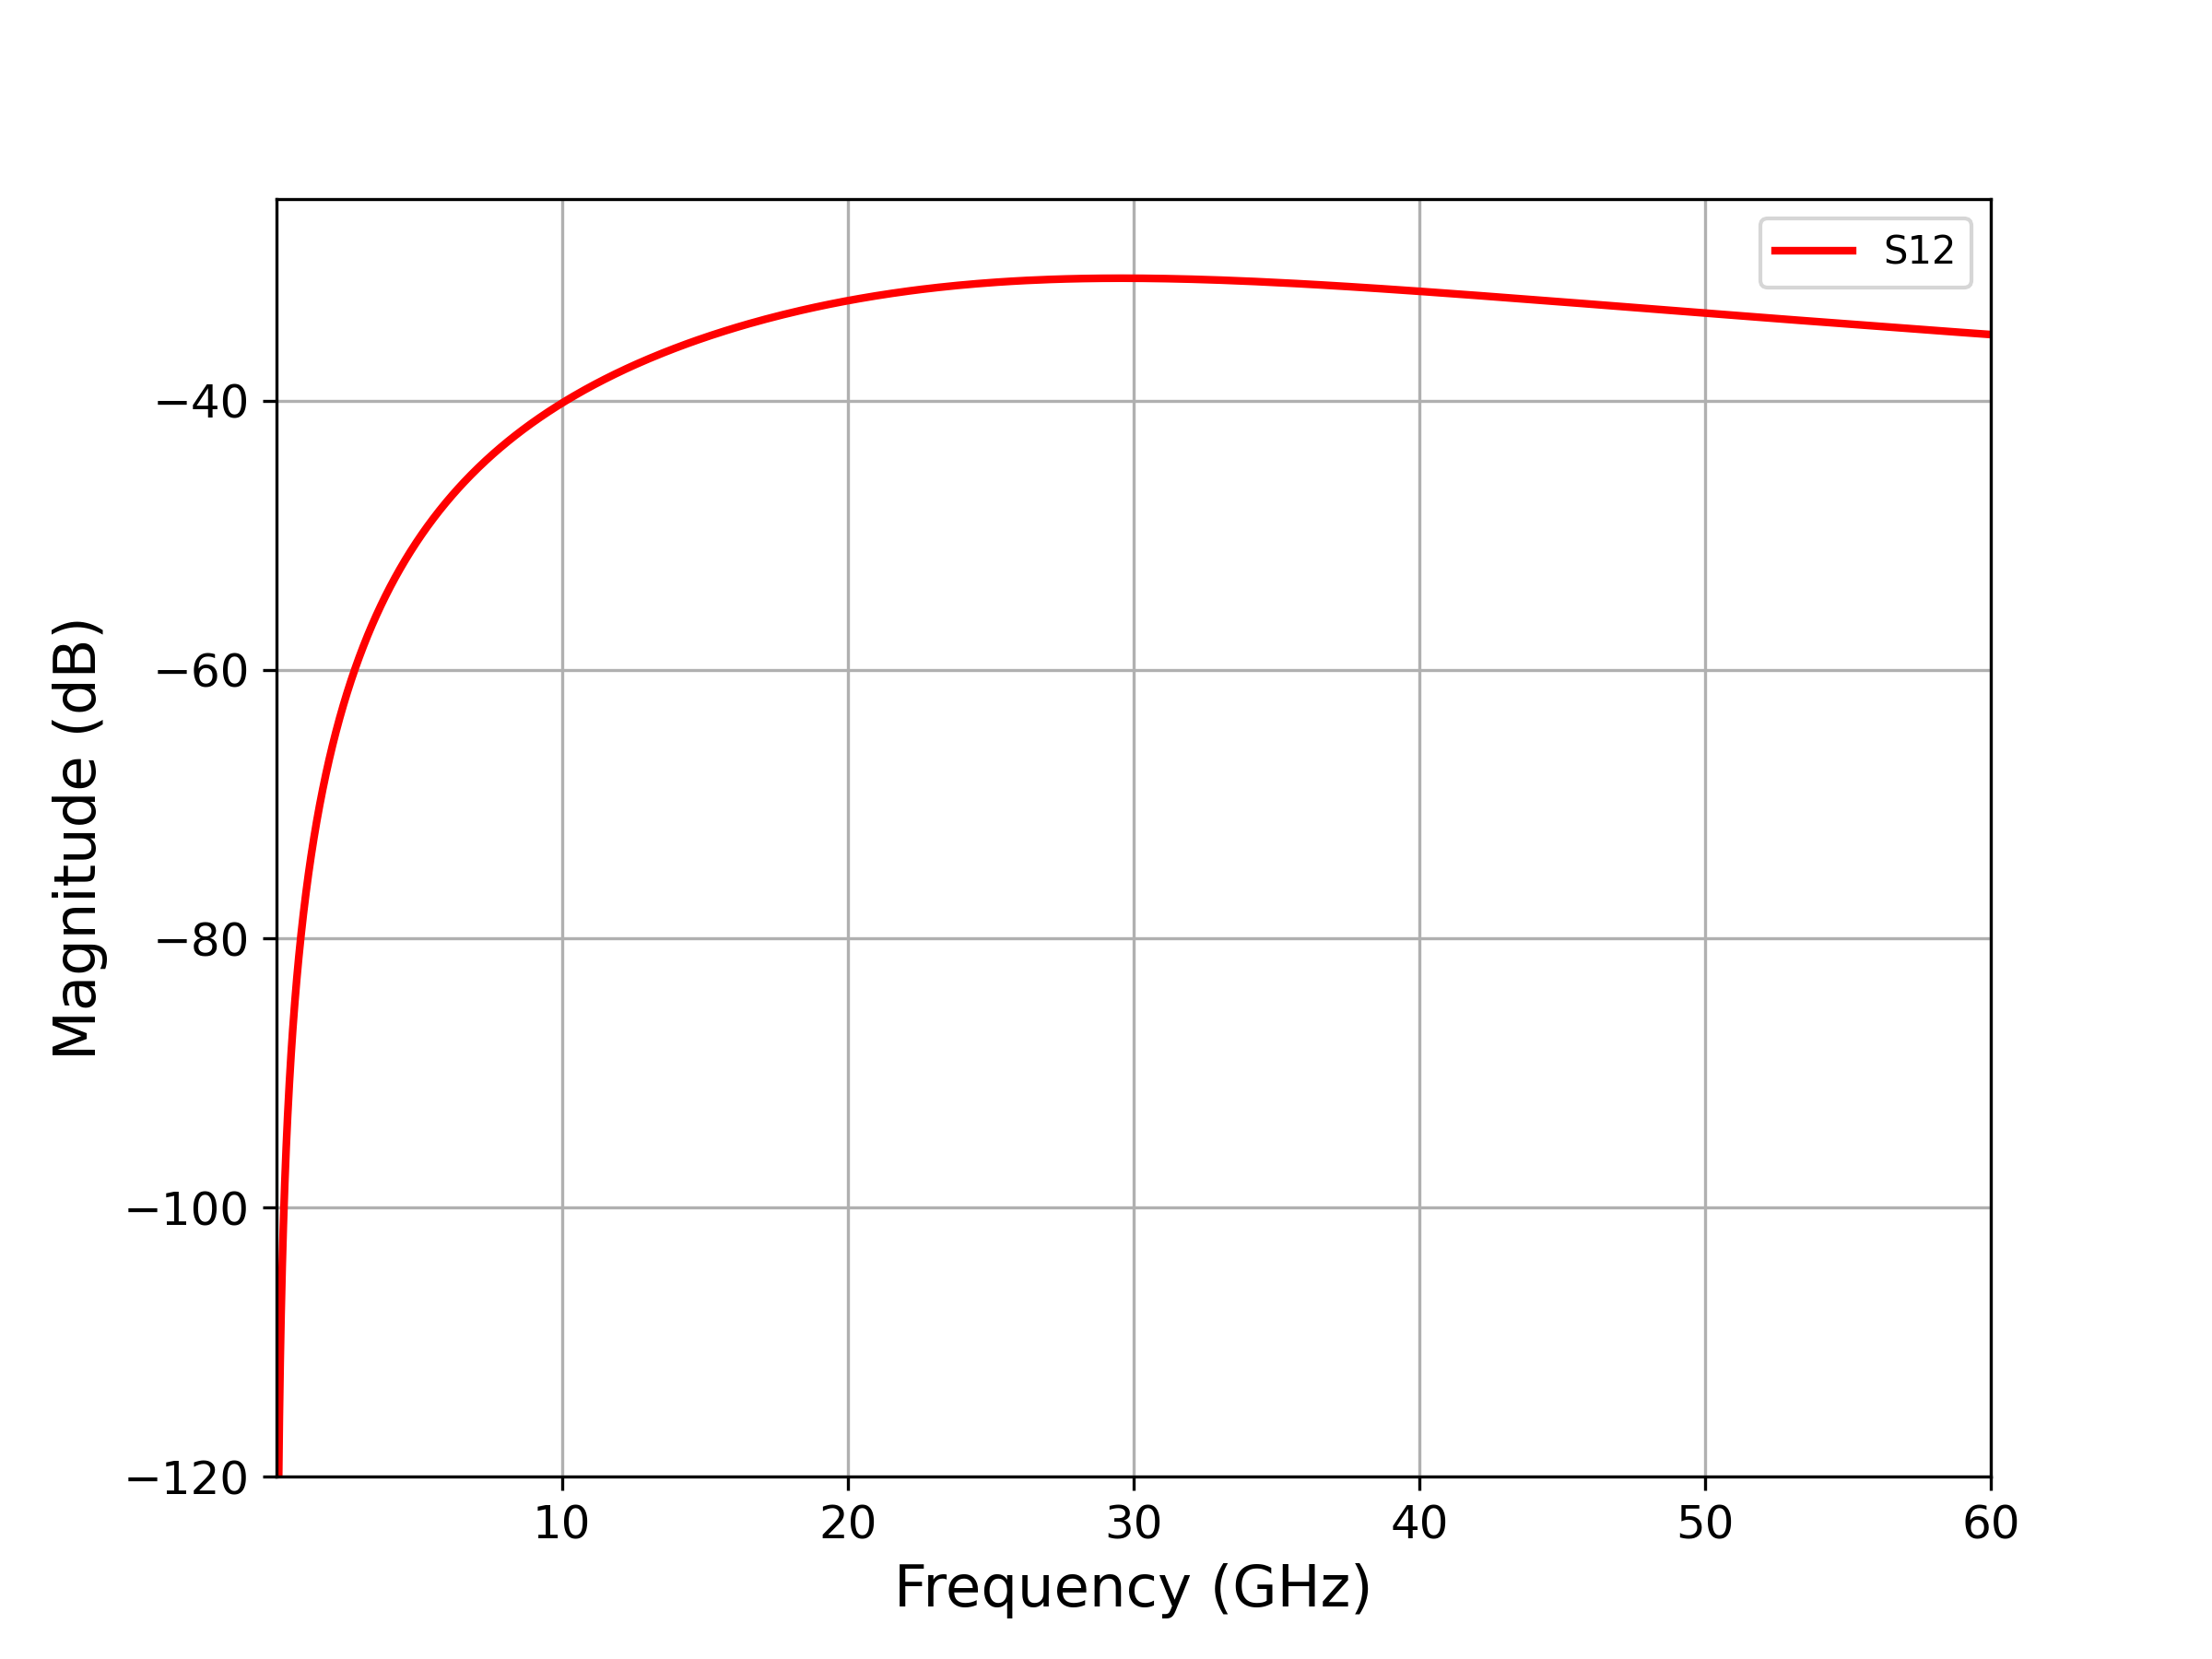
\includegraphics[width=\linewidth]{figures/single_stage_s12.png}
    \caption{}
     \label{fig:single-stage-without-cadence-s12}
  \end{subfigure}
  \caption{(a) $S_{11}$ parameter of a single-stage power amplifier (shown in Figure \ref{fig:single-stage-power-amplifier}) without matching network. (b) $S_{12}$ parameter of a single-stage power amplifier (shown in Figure \ref{fig:single-stage-power-amplifier}) without matching network.}
  \label{fig:single-stage-without-cadence-s11-s12}
\end{figure}

The value of $S_{11}$ of a single-stage power amplifier is -0.17 dB at frequency 18 GHz, which indicates poor input matching. This means a significant portion of the power is being reflected back rather than absorbed by the amplifier, leading to inefficiency. The Return Loss ($S_{12}$) parameter represents the power reflected back from Port 2 (the incident signal) to Port 1 (the reflected signal) in a two-port network. The value of $S_{12}$ a single-stage power amplifier is less than -30 dB through the BW.
% \begin{figure}[H]
%     \centering
%     \resizebox{0.8\textwidth}{!}{
%     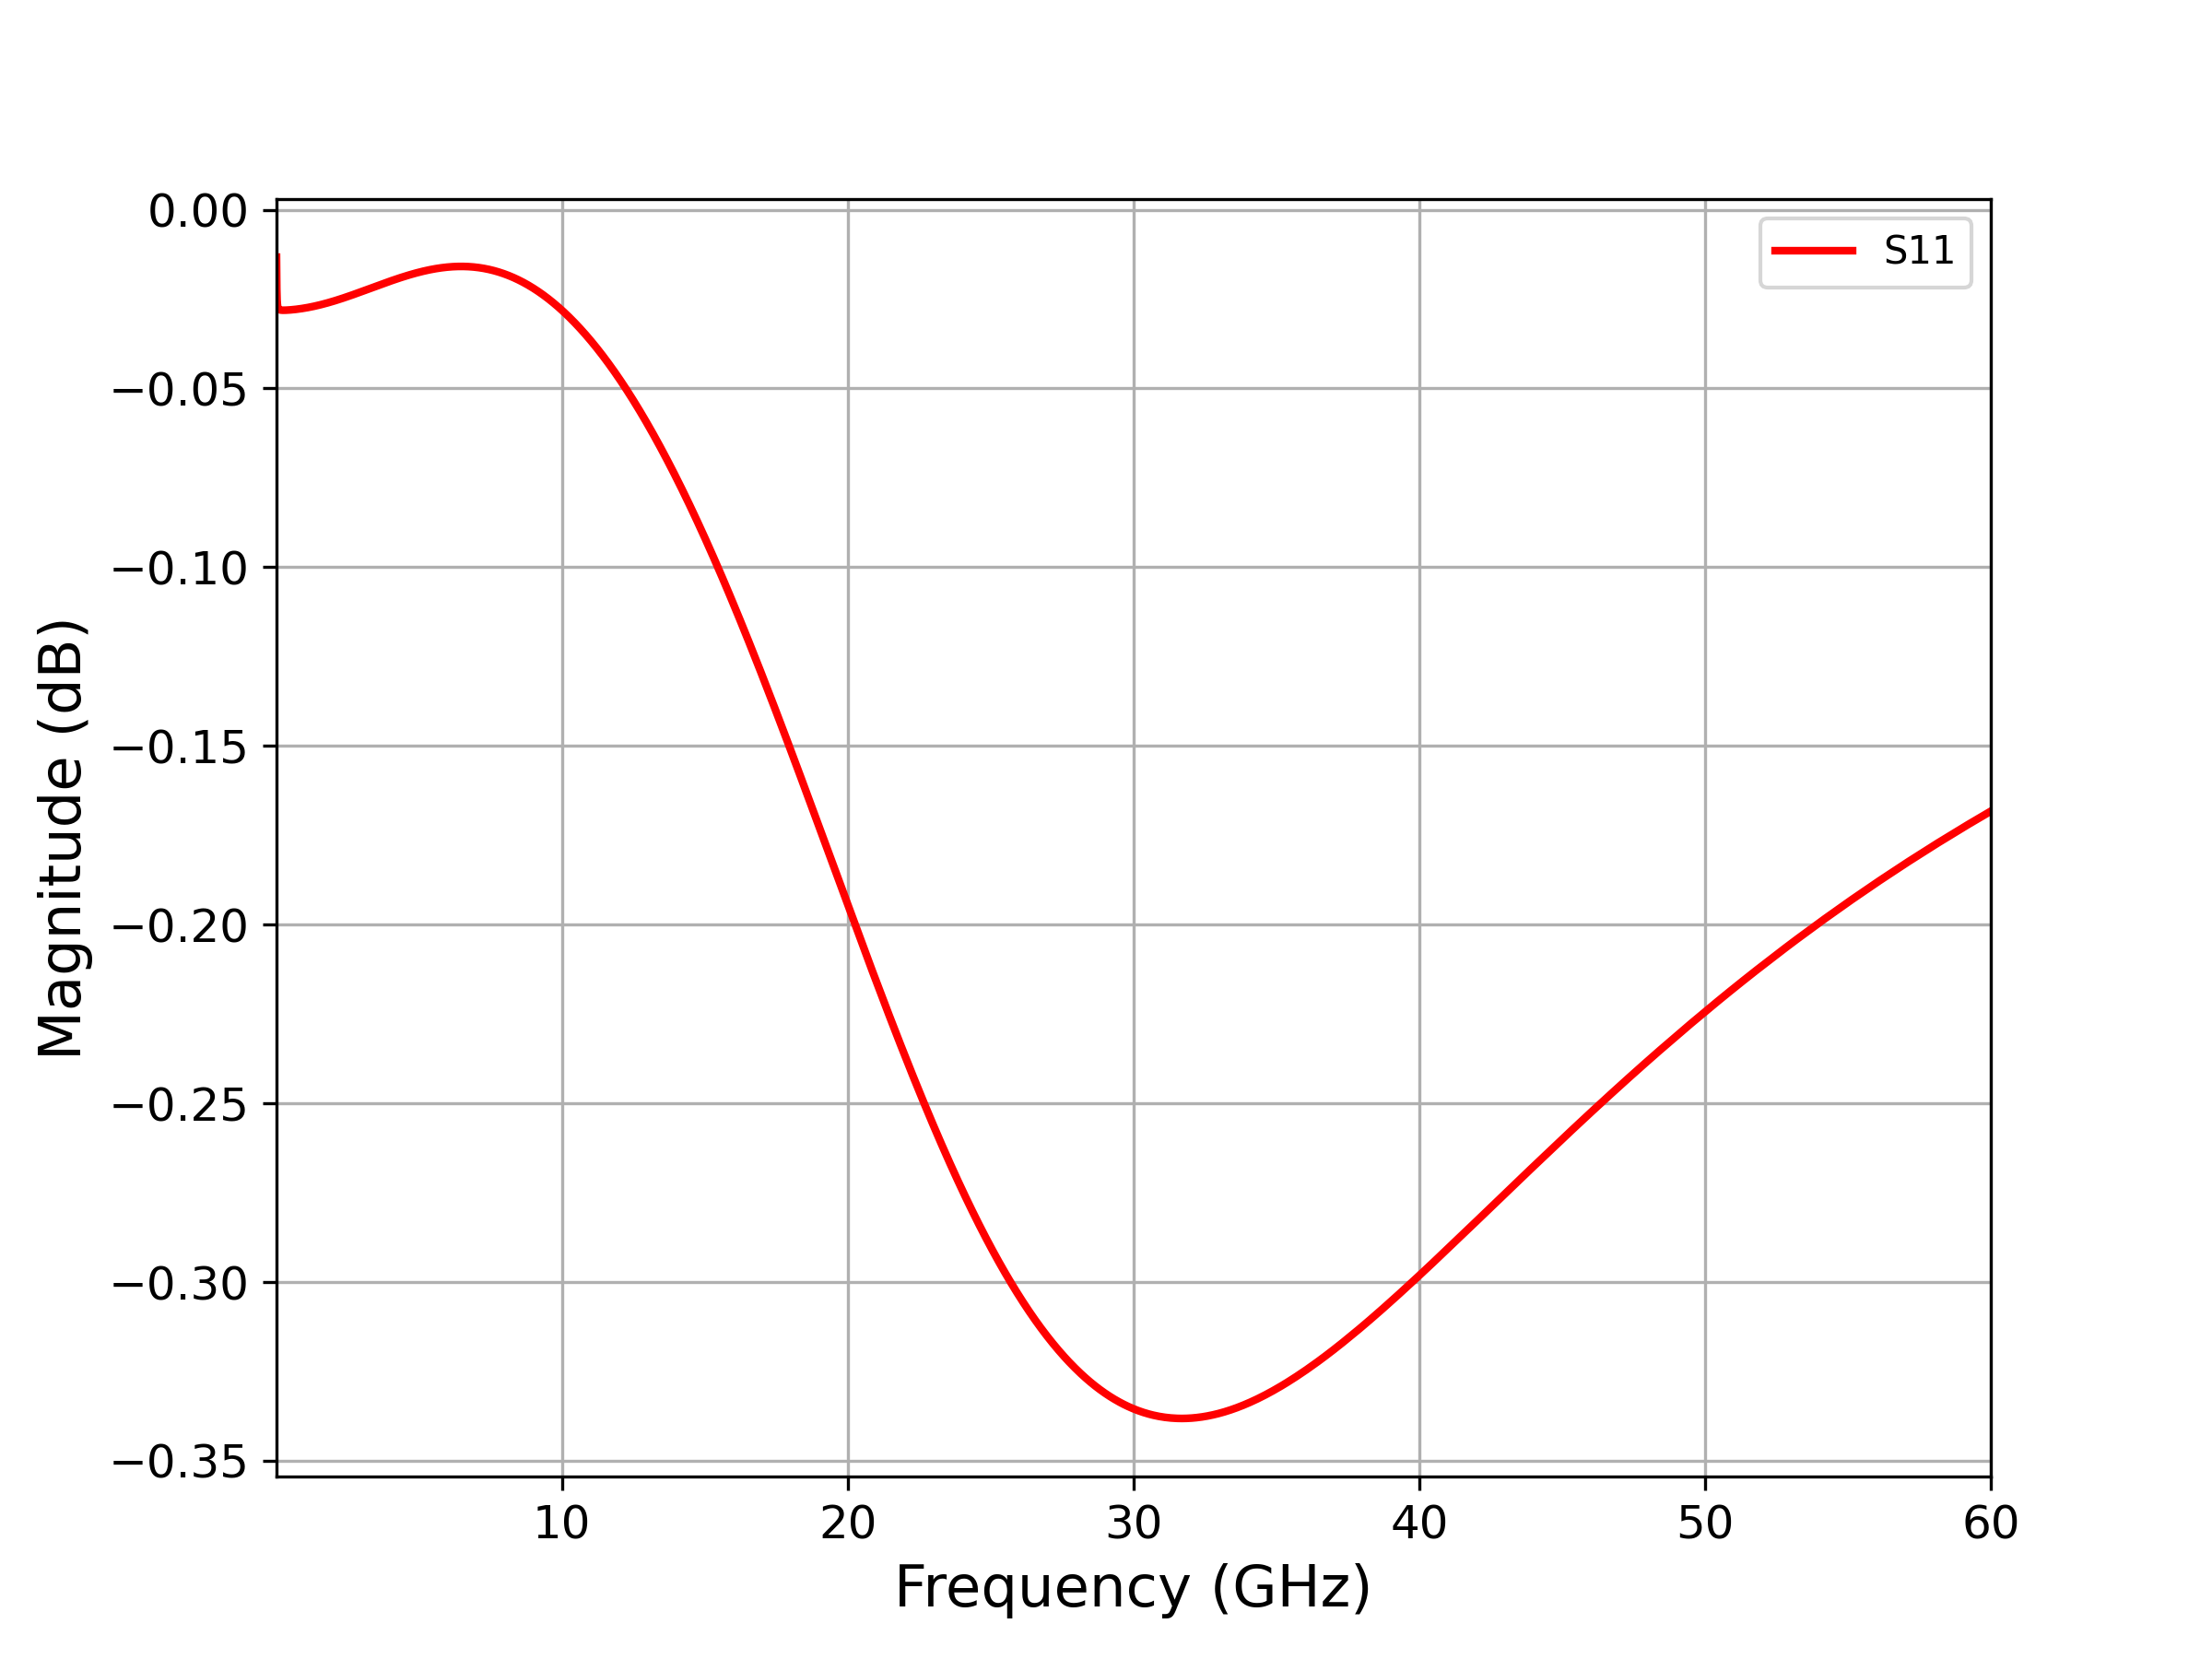
\includegraphics[]{figures/single_stage_s11.png}
%     }
%     \caption{$S_{11}$ parameter of a single-stage power amplifier (shown in Figure \ref{fig:single-stage-power-amplifier}) without matching network. The $S_{11}$ parameter is plotted from 0 GHz to 60 GHz.}
%     \label{fig:single-stage-without-cadence-s11}
% \end{figure}
% \begin{figure}[H]
%     \centering
%     \resizebox{0.8\textwidth}{!}{
%     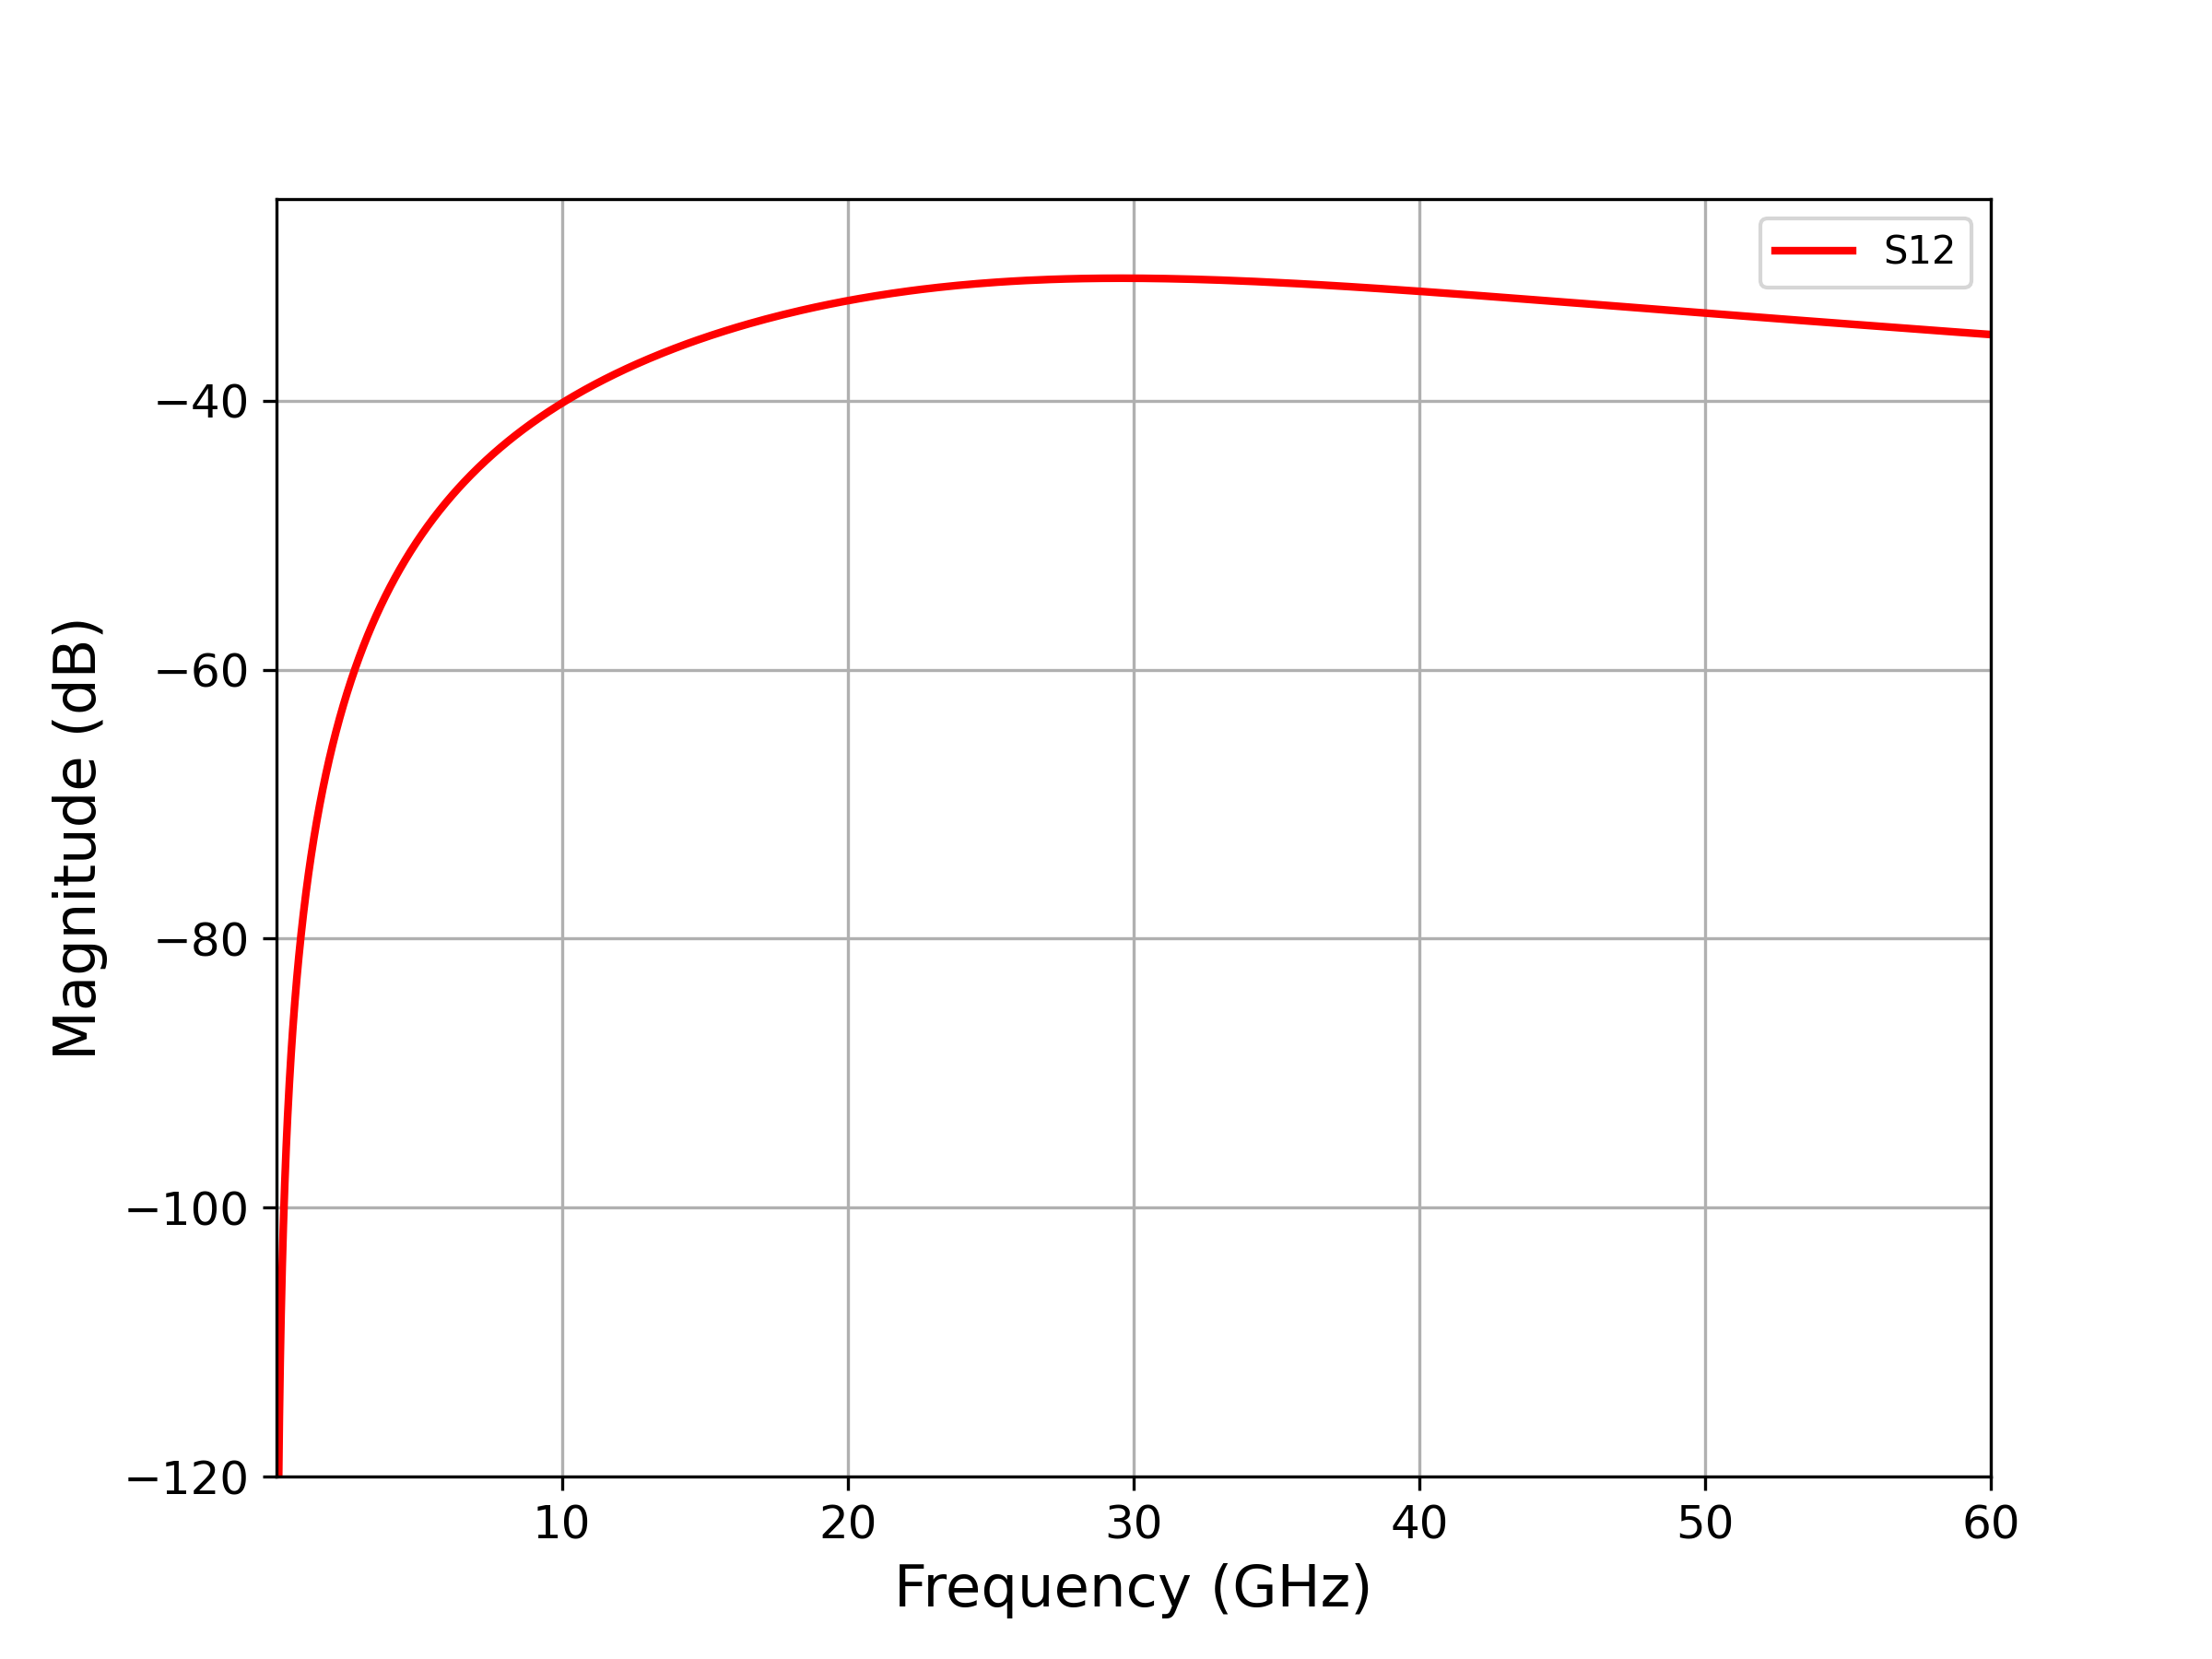
\includegraphics[]{figures/single_stage_s12.png}
%     }
%     \caption{$S_{12}$ parameter of a single-stage power amplifier (shown in Figure \ref{fig:single-stage-power-amplifier}) without matching network. The $S_{12}$ parameter is plotted from 0 GHz to 60 GHz.}
%     \label{fig:single-stage-without-cadence-s12}
% \end{figure}
\begin{figure}[H]
  \centering
  \begin{subfigure}{0.49\textwidth}
    \centering
    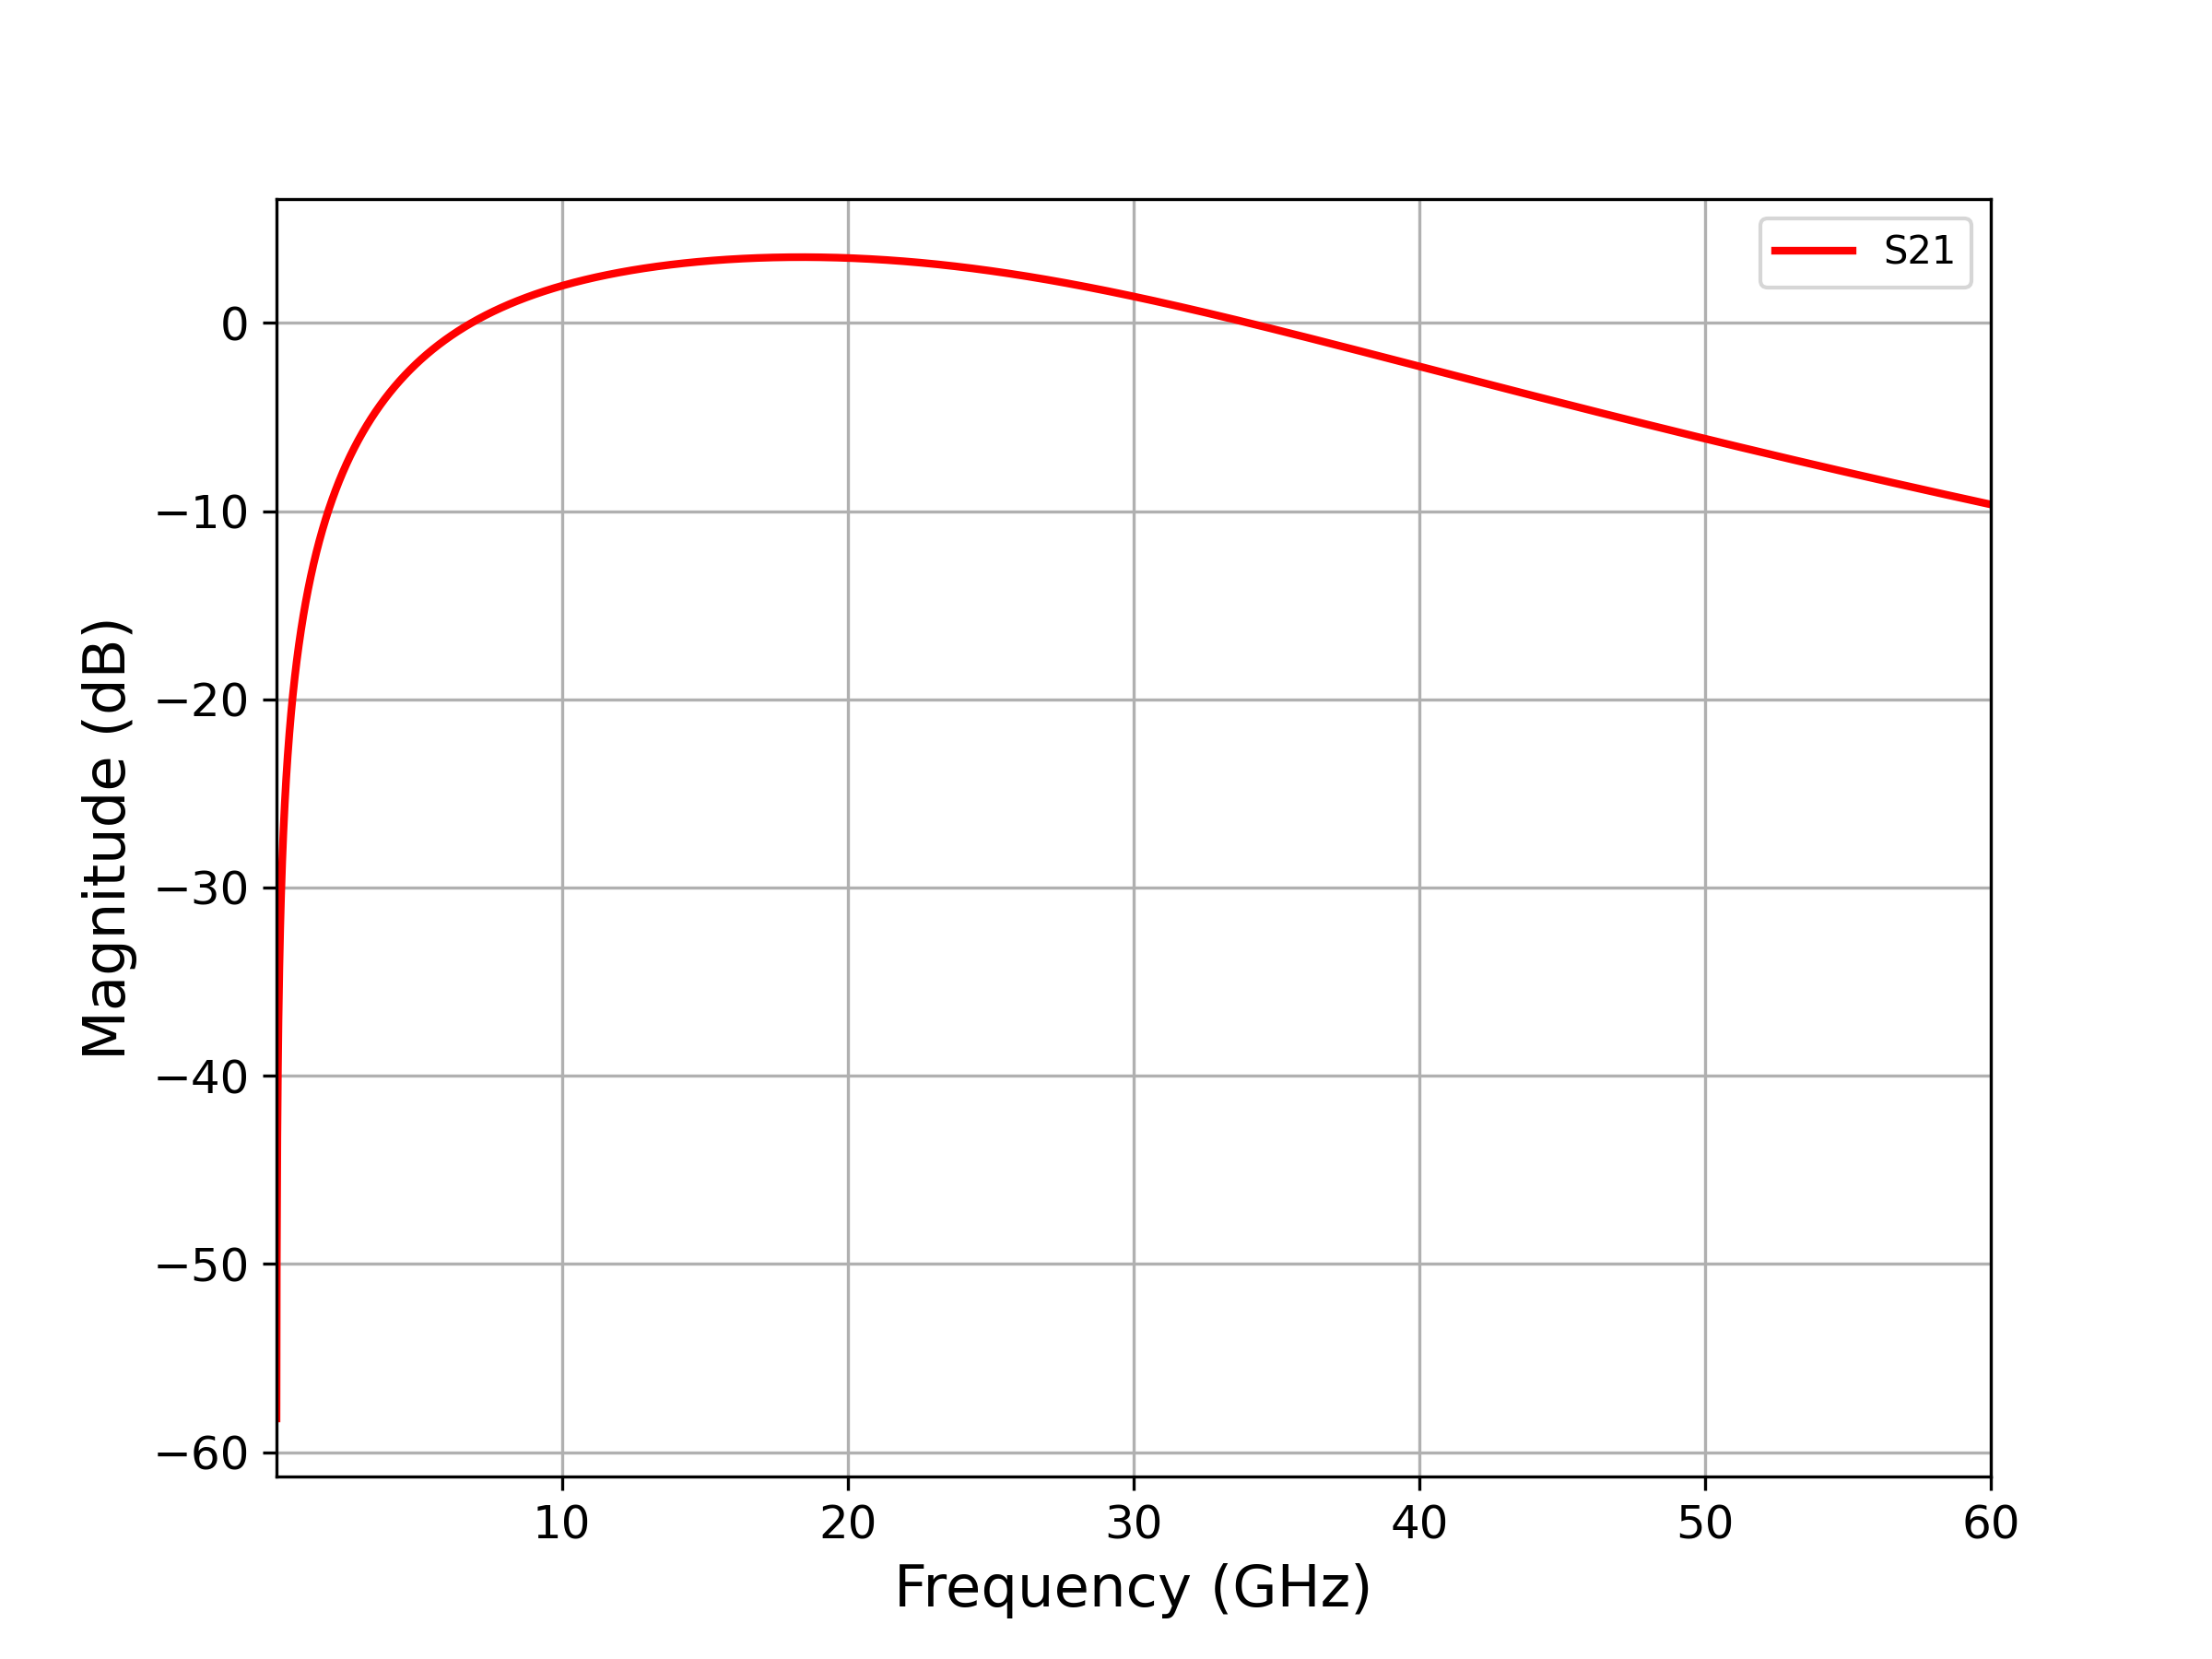
\includegraphics[width=\linewidth]{figures/single_stage_s21.png}
    \caption{}
    \label{fig:single-stage-without-cadence-s21}
  \end{subfigure}
  \hfill
  \begin{subfigure}{0.49\textwidth}
    \centering
    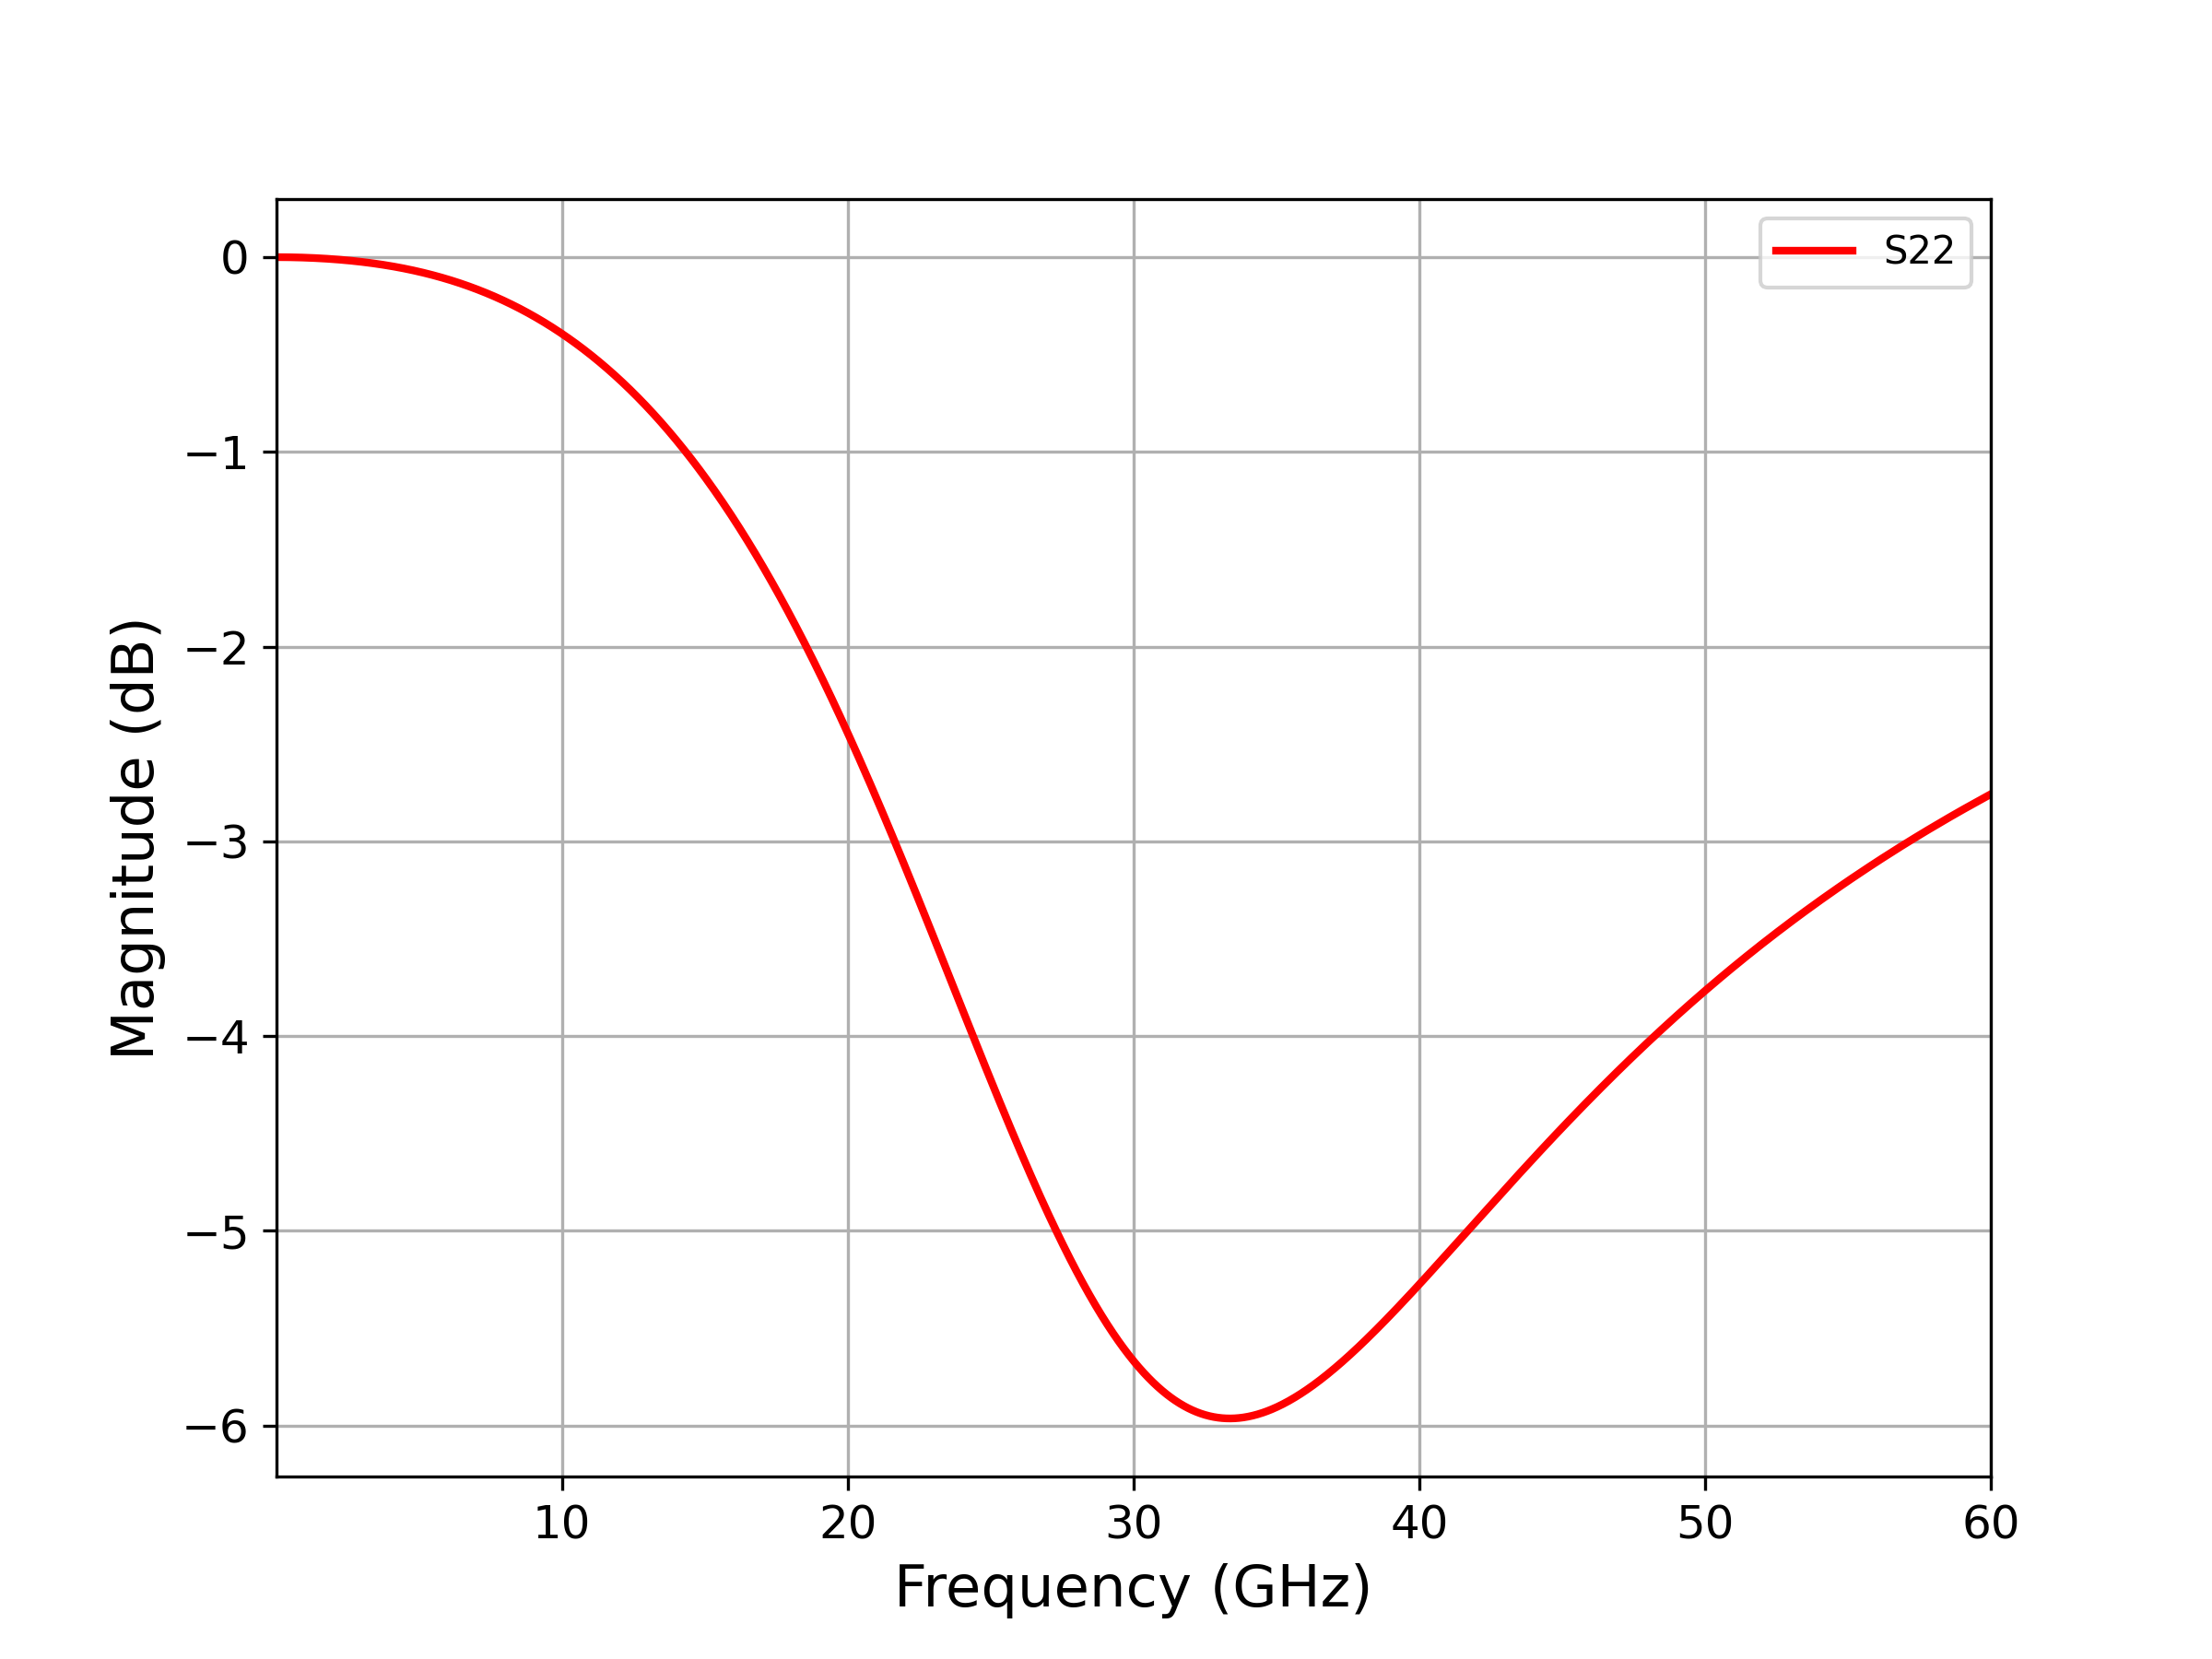
\includegraphics[width=\linewidth]{figures/single_stage_s22.png}
    \caption{}
     \label{fig:single-stage-without-cadence-s22}
  \end{subfigure}
  \caption{(a) $S_{21}$ parameter of a single-stage power amplifier (shown in Figure \ref{fig:single-stage-power-amplifier}) without matching network. (b) $S_{22}$ parameter of a single-stage power amplifier (shown in Figure \ref{fig:single-stage-power-amplifier}) without matching network.}
  \label{fig:single-stage-without-cadence-s21-s22}
\end{figure}

The maximum value of $S_{21}$ of a single-stage power amplifier is 3.78 dB at resonance frequency 18 GHz, which indicates poor power gain, which is not enough for real-life applications. The $S_{22}$ parameter is a measure of how well the power amplifier matches the impedance at its output. A lower magnitude of 
$S_{22}$ indicates a better match between the output impedance of the power amplifier and the load impedance, resulting in less power being reflected back. A higher magnitude indicates a higher level of reflection and poor impedance matching. The value of $S_{22}$ of single-stage PA is -1.9 dB at 18 GHz, which is insufficient for an output-matching network. 
% \begin{figure}[H]
%     \centering
%     \resizebox{0.8\textwidth}{!}{
%     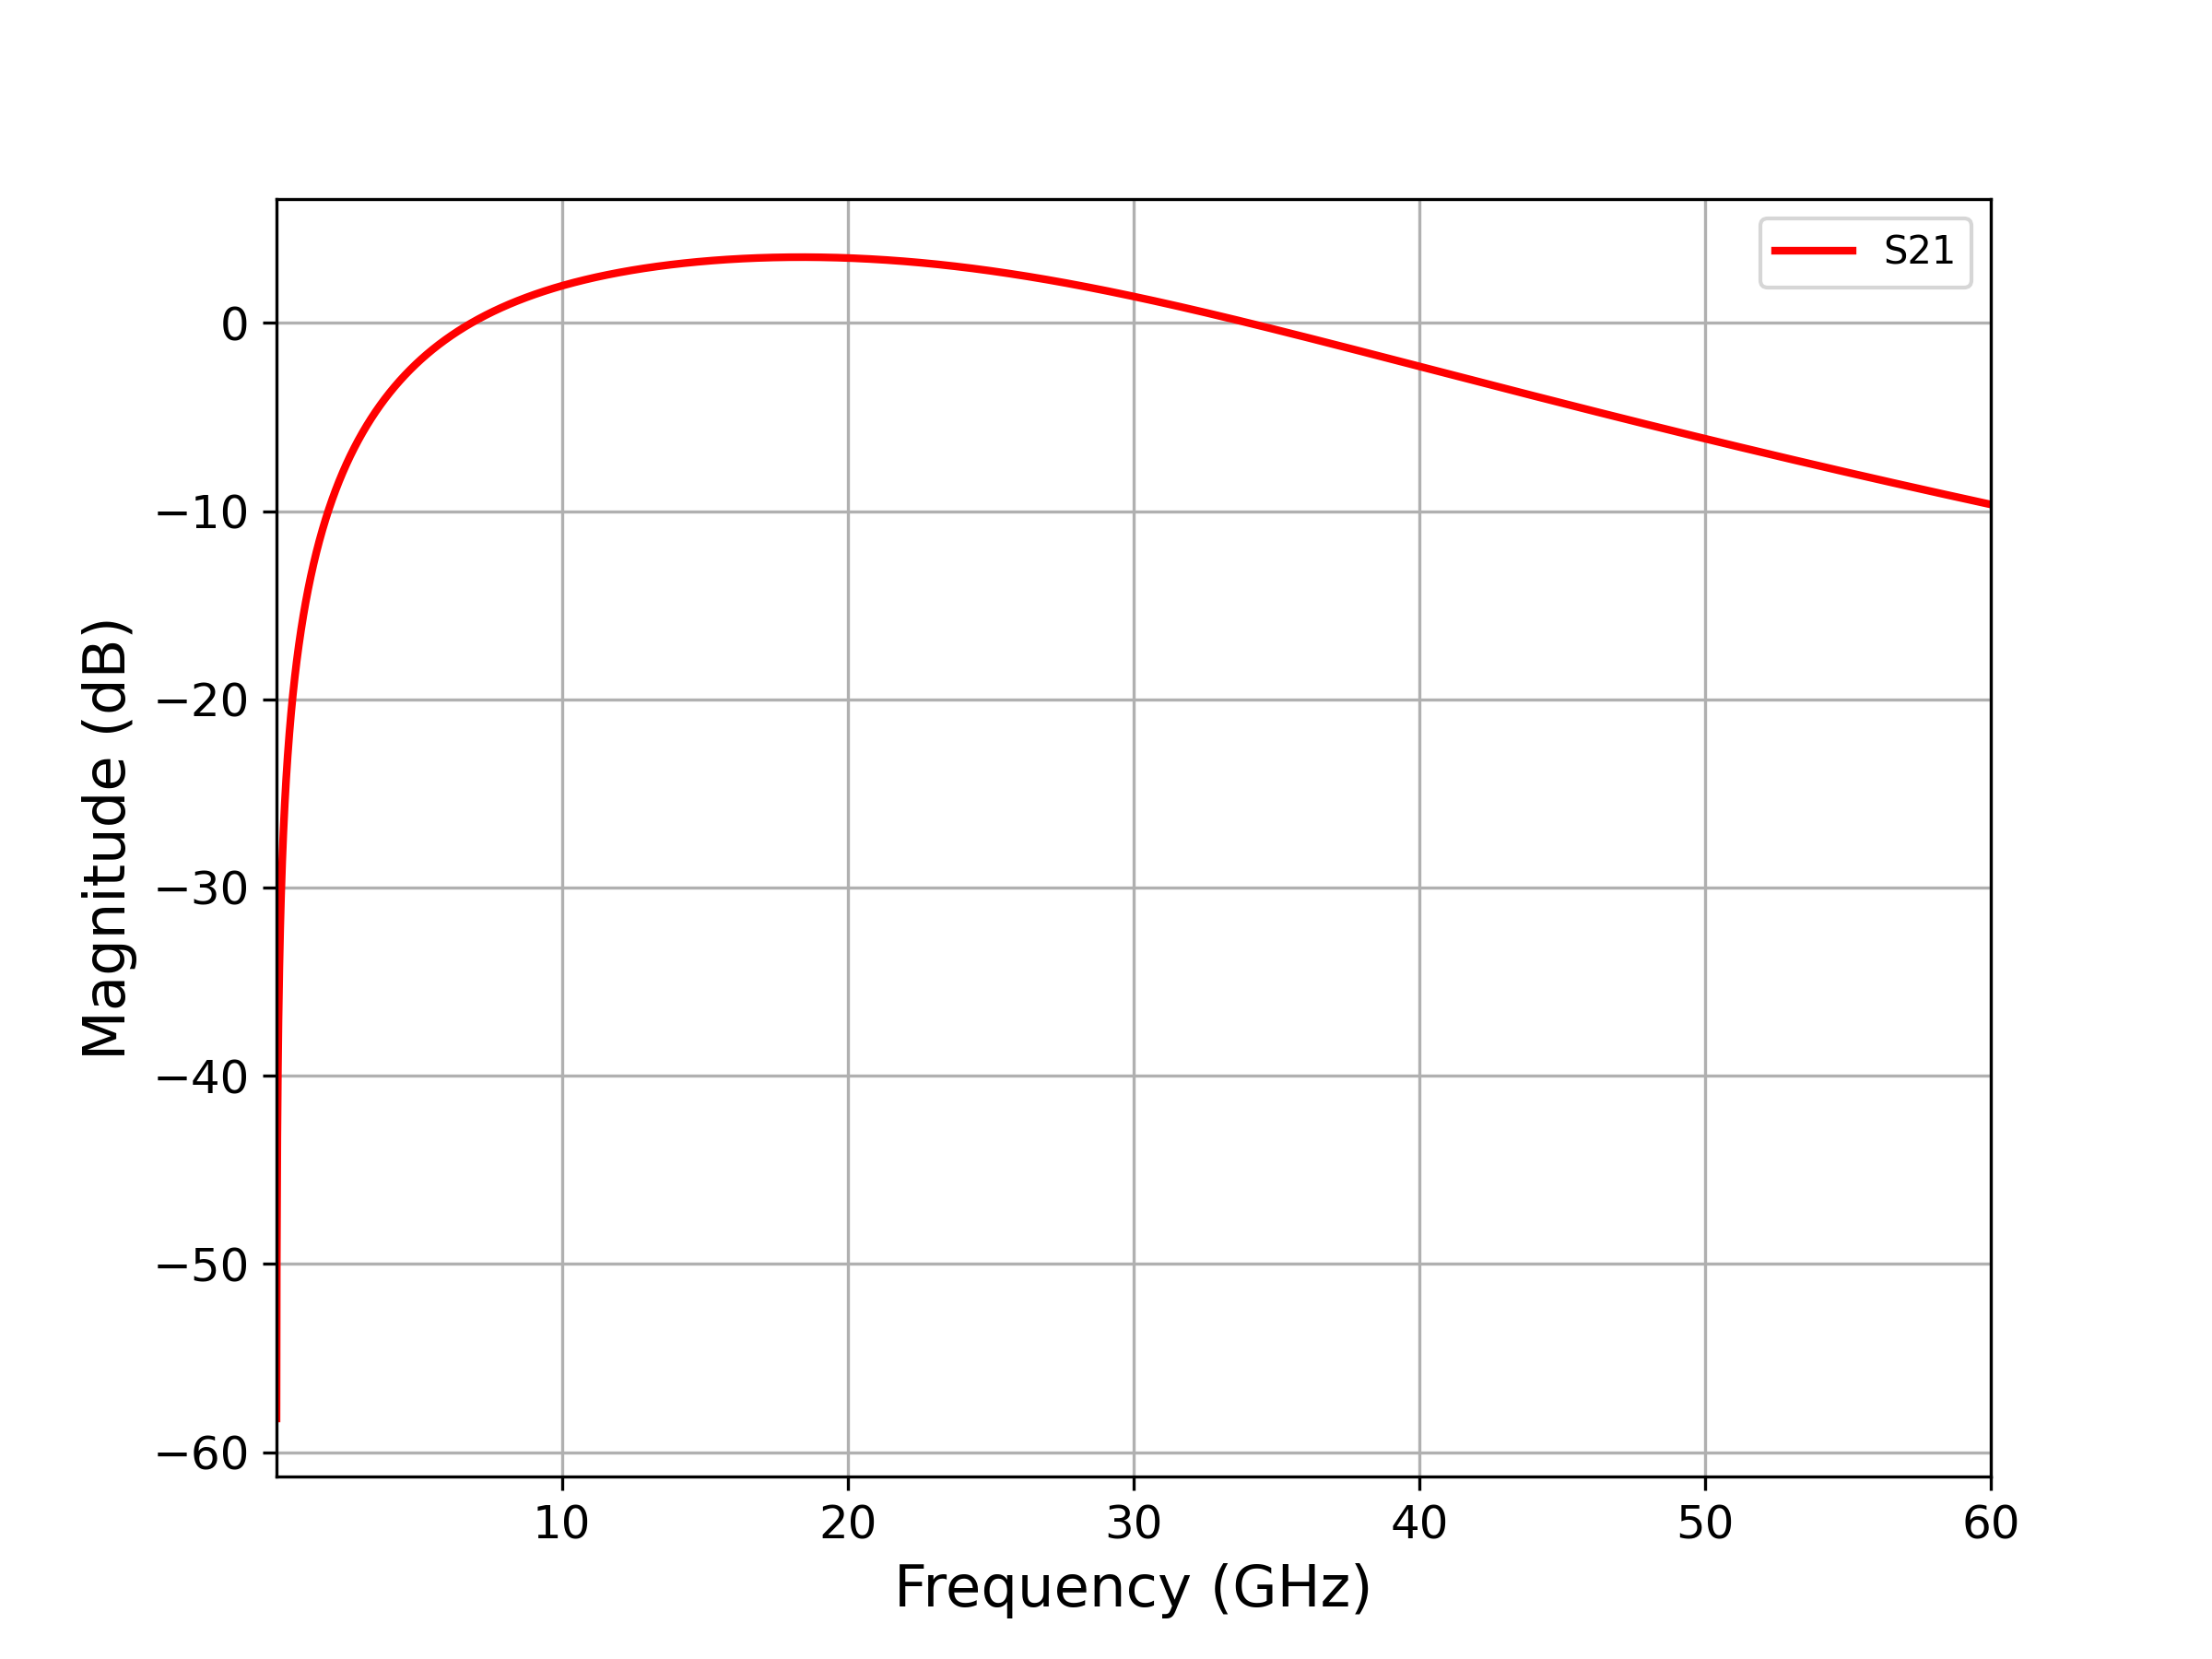
\includegraphics[]{figures/single_stage_s21.png}
%     }
%     \caption{$S_{21}$ parameter of a single-stage power amplifier (shown in Figure \ref{fig:single-stage-power-amplifier}) without matching network. The $S_{21}$ parameter is plotted from 0 GHz to 60 GHz.}
%     \label{fig:single-stage-without-cadence-s21}
% \end{figure}
% \begin{figure}[H]
%     \centering
%     \resizebox{0.8\textwidth}{!}{
%     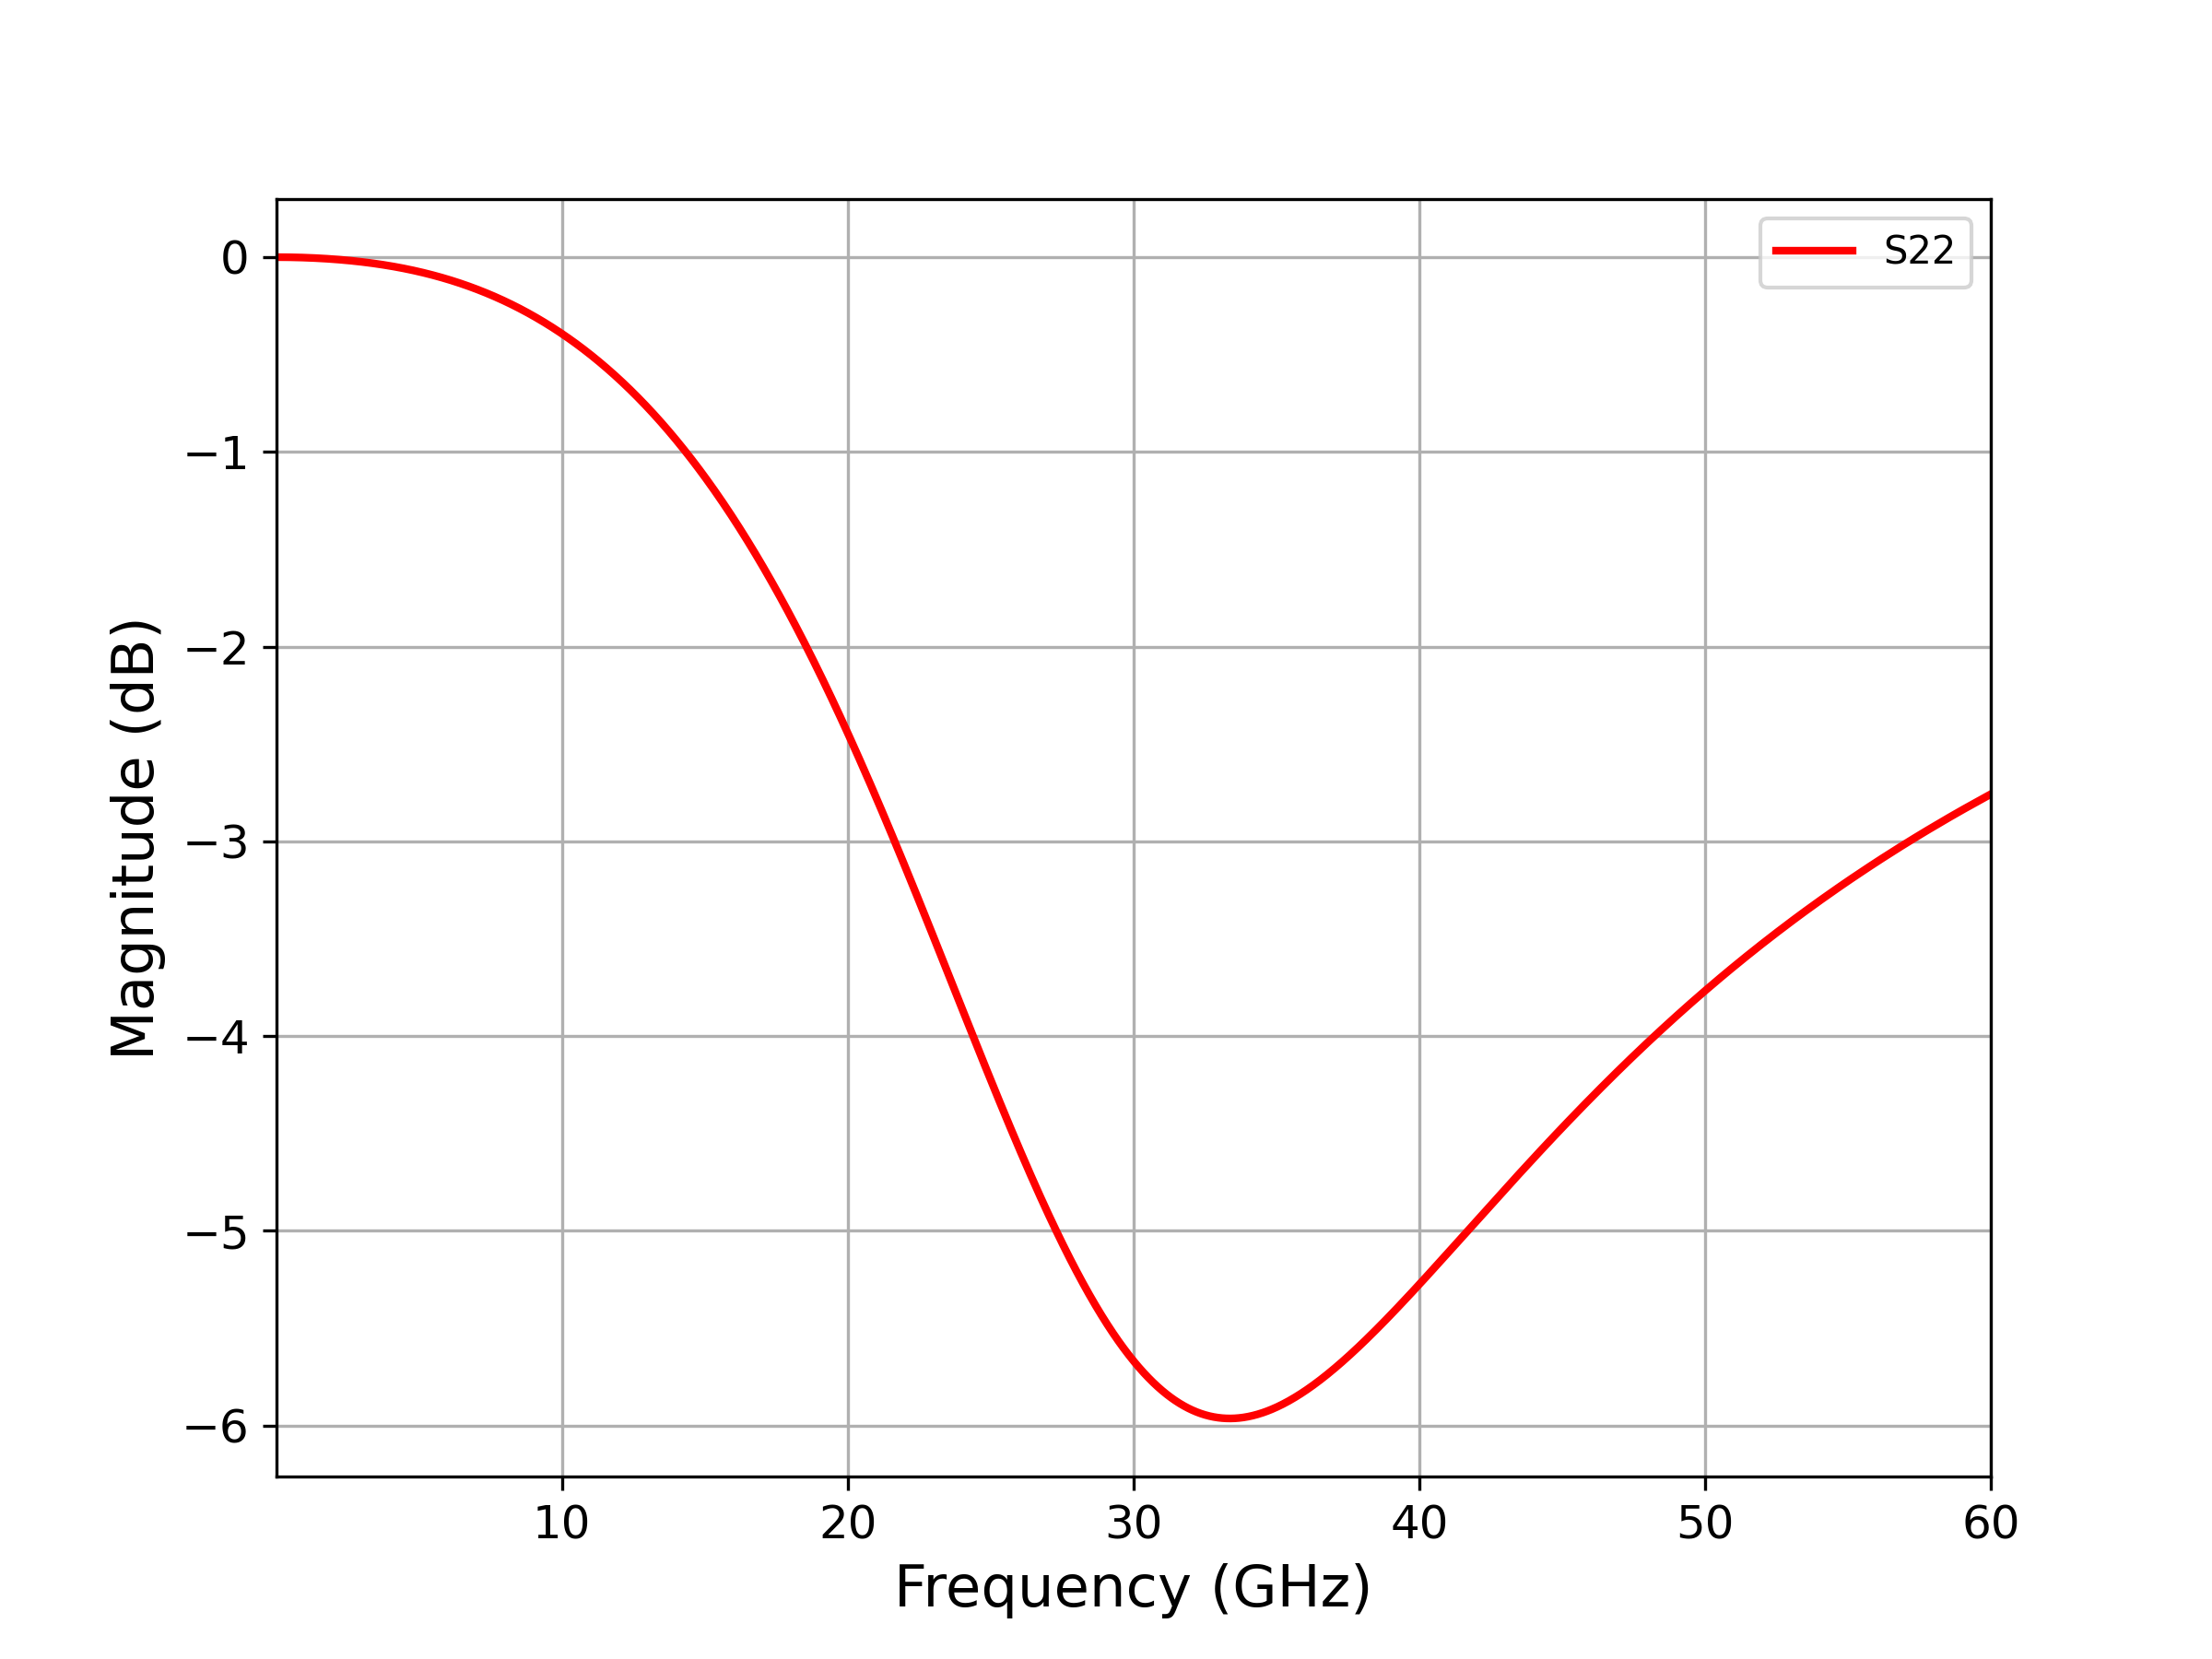
\includegraphics[]{figures/single_stage_s22.png}
%     }
%     \caption{$S_{22}$ parameter of a single-stage power amplifier (shown in Figure \ref{fig:single-stage-power-amplifier}) without matching network. The $S_{22}$ parameter is plotted from 0 GHz to 60 GHz.}
%     \label{fig:single-stage-without-cadence-s22}
% \end{figure}

%The $S$ parameter simulation of two stage power amplifier(Figure \ref{fig:double-stage-power-amplifier}) is shown below
\begin{figure}[H]
  \centering
  \begin{subfigure}{0.49\textwidth}
    \centering
    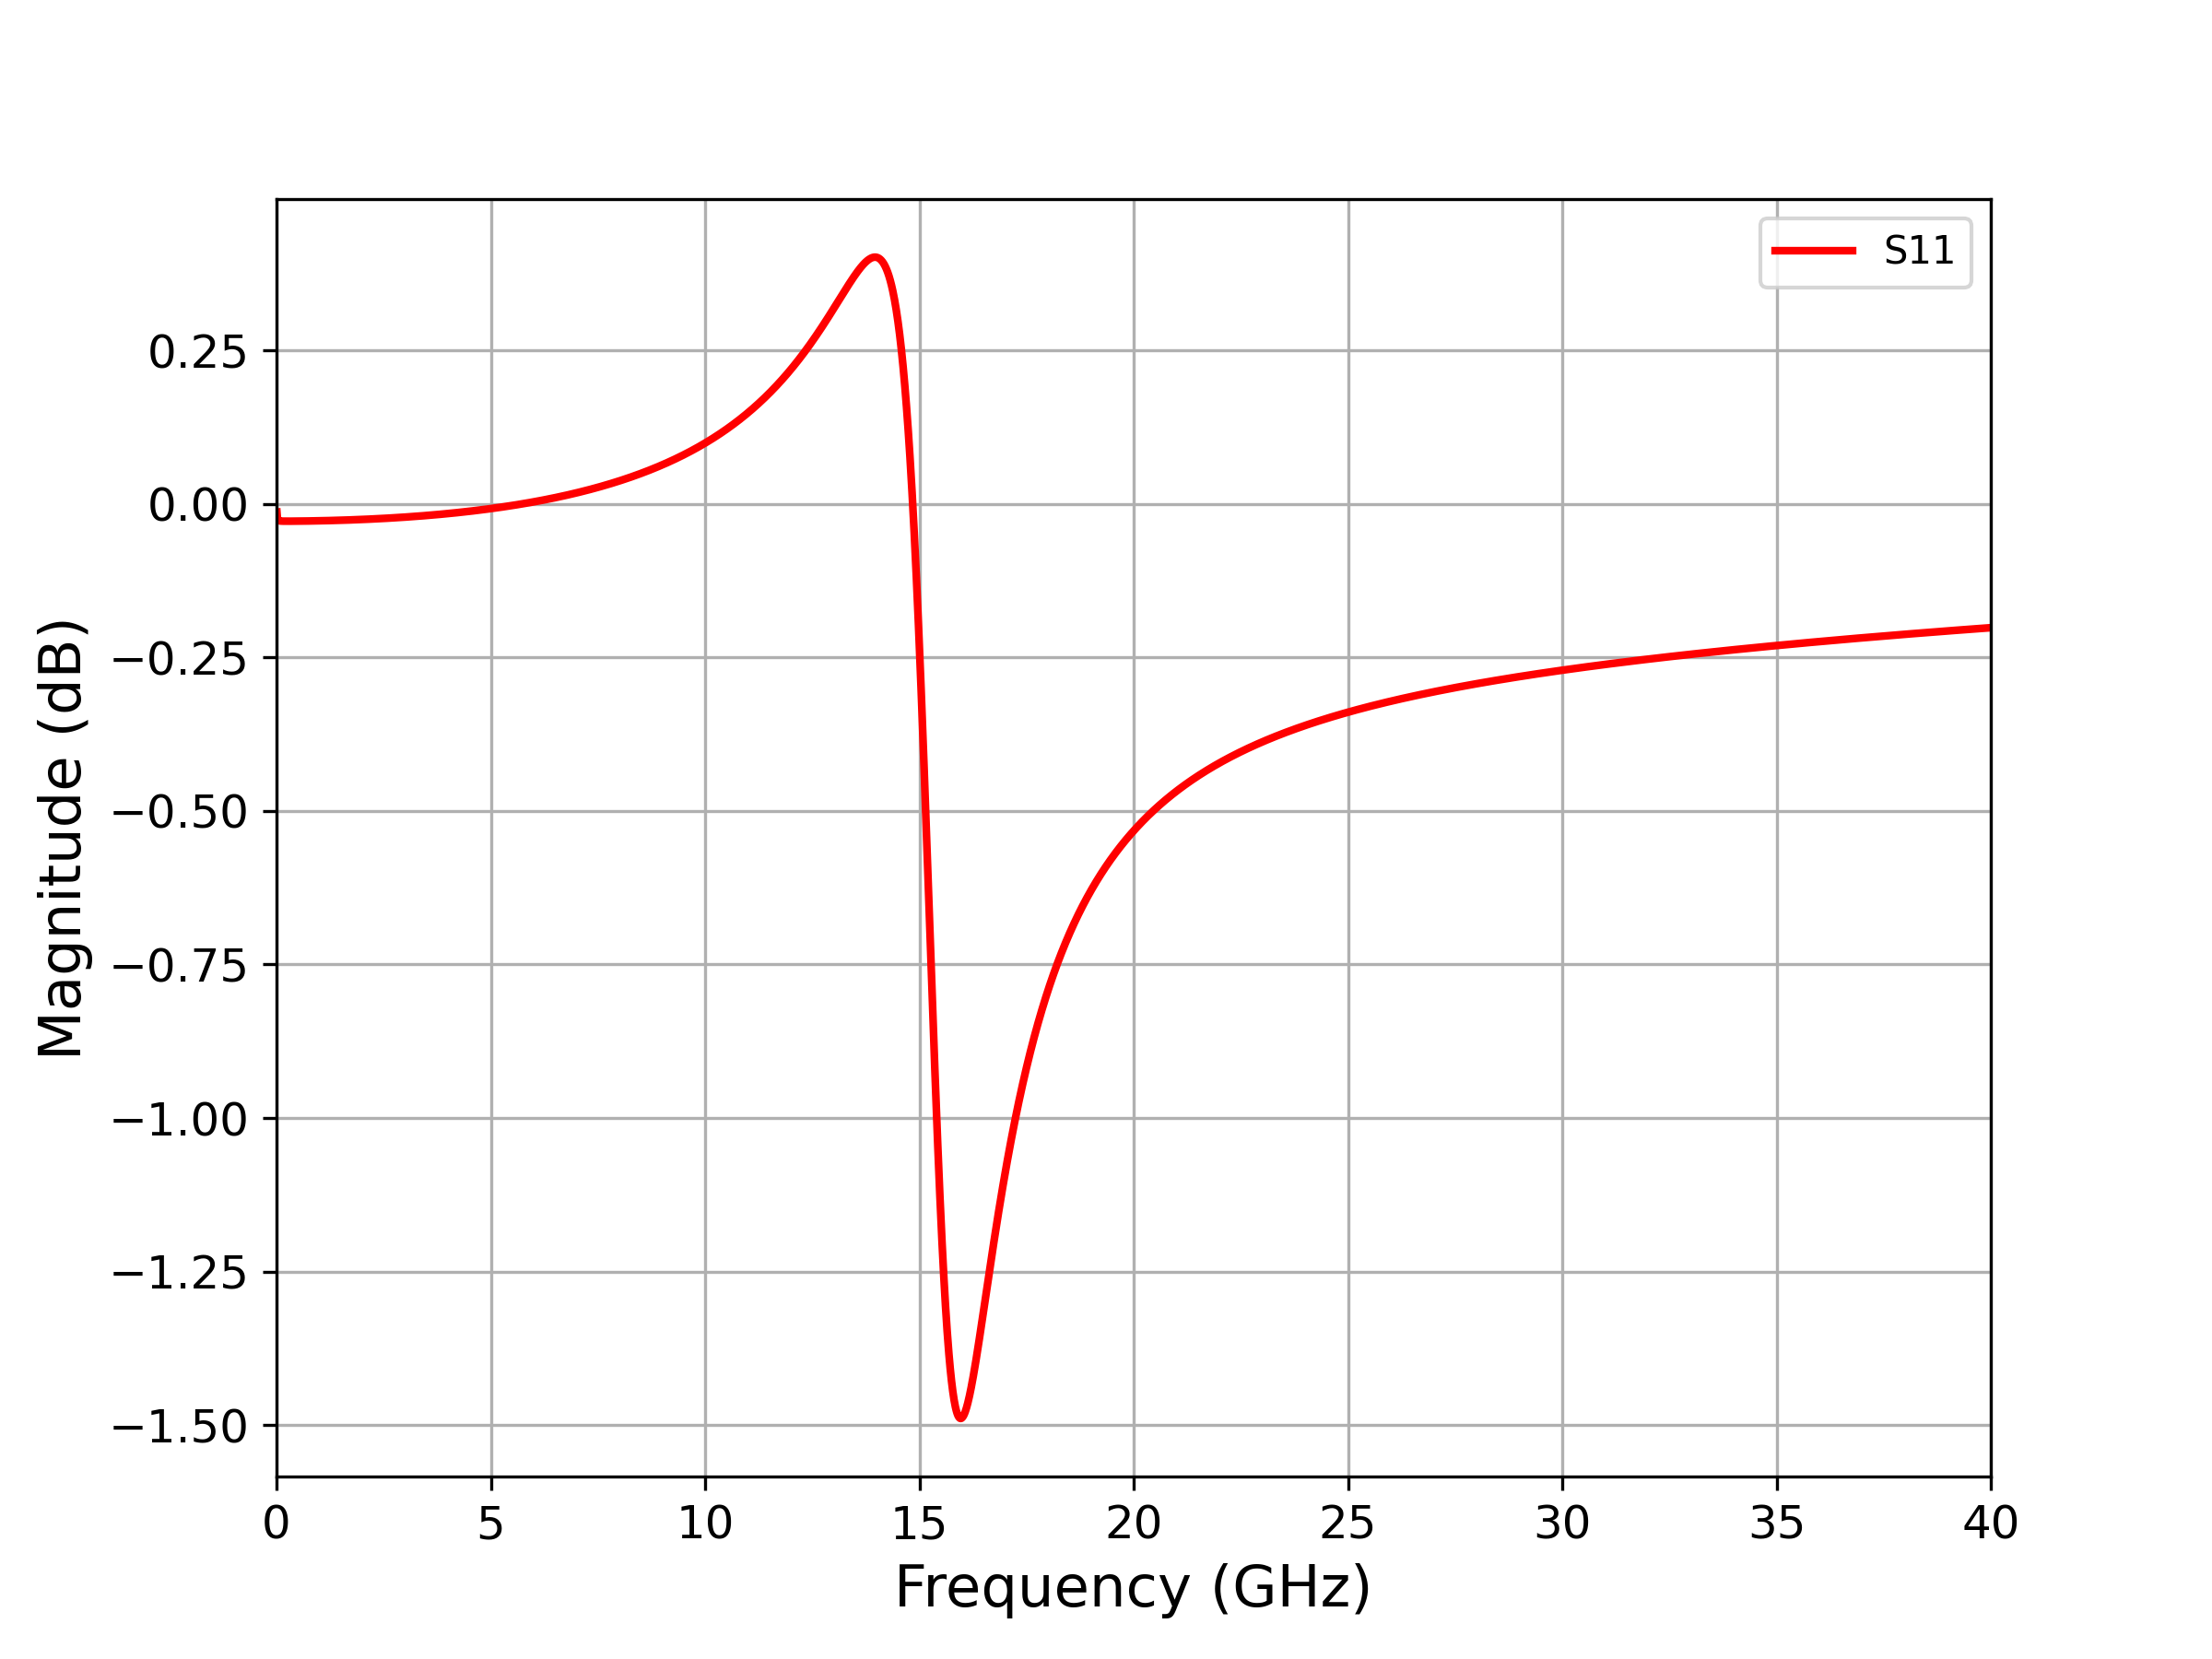
\includegraphics[width=\linewidth]{figures/two_stage_s11.png}
    \caption{}
    \label{fig:two-stage-without-cadence-s11}
  \end{subfigure}
  \hfill
  \begin{subfigure}{0.49\textwidth}
    \centering
    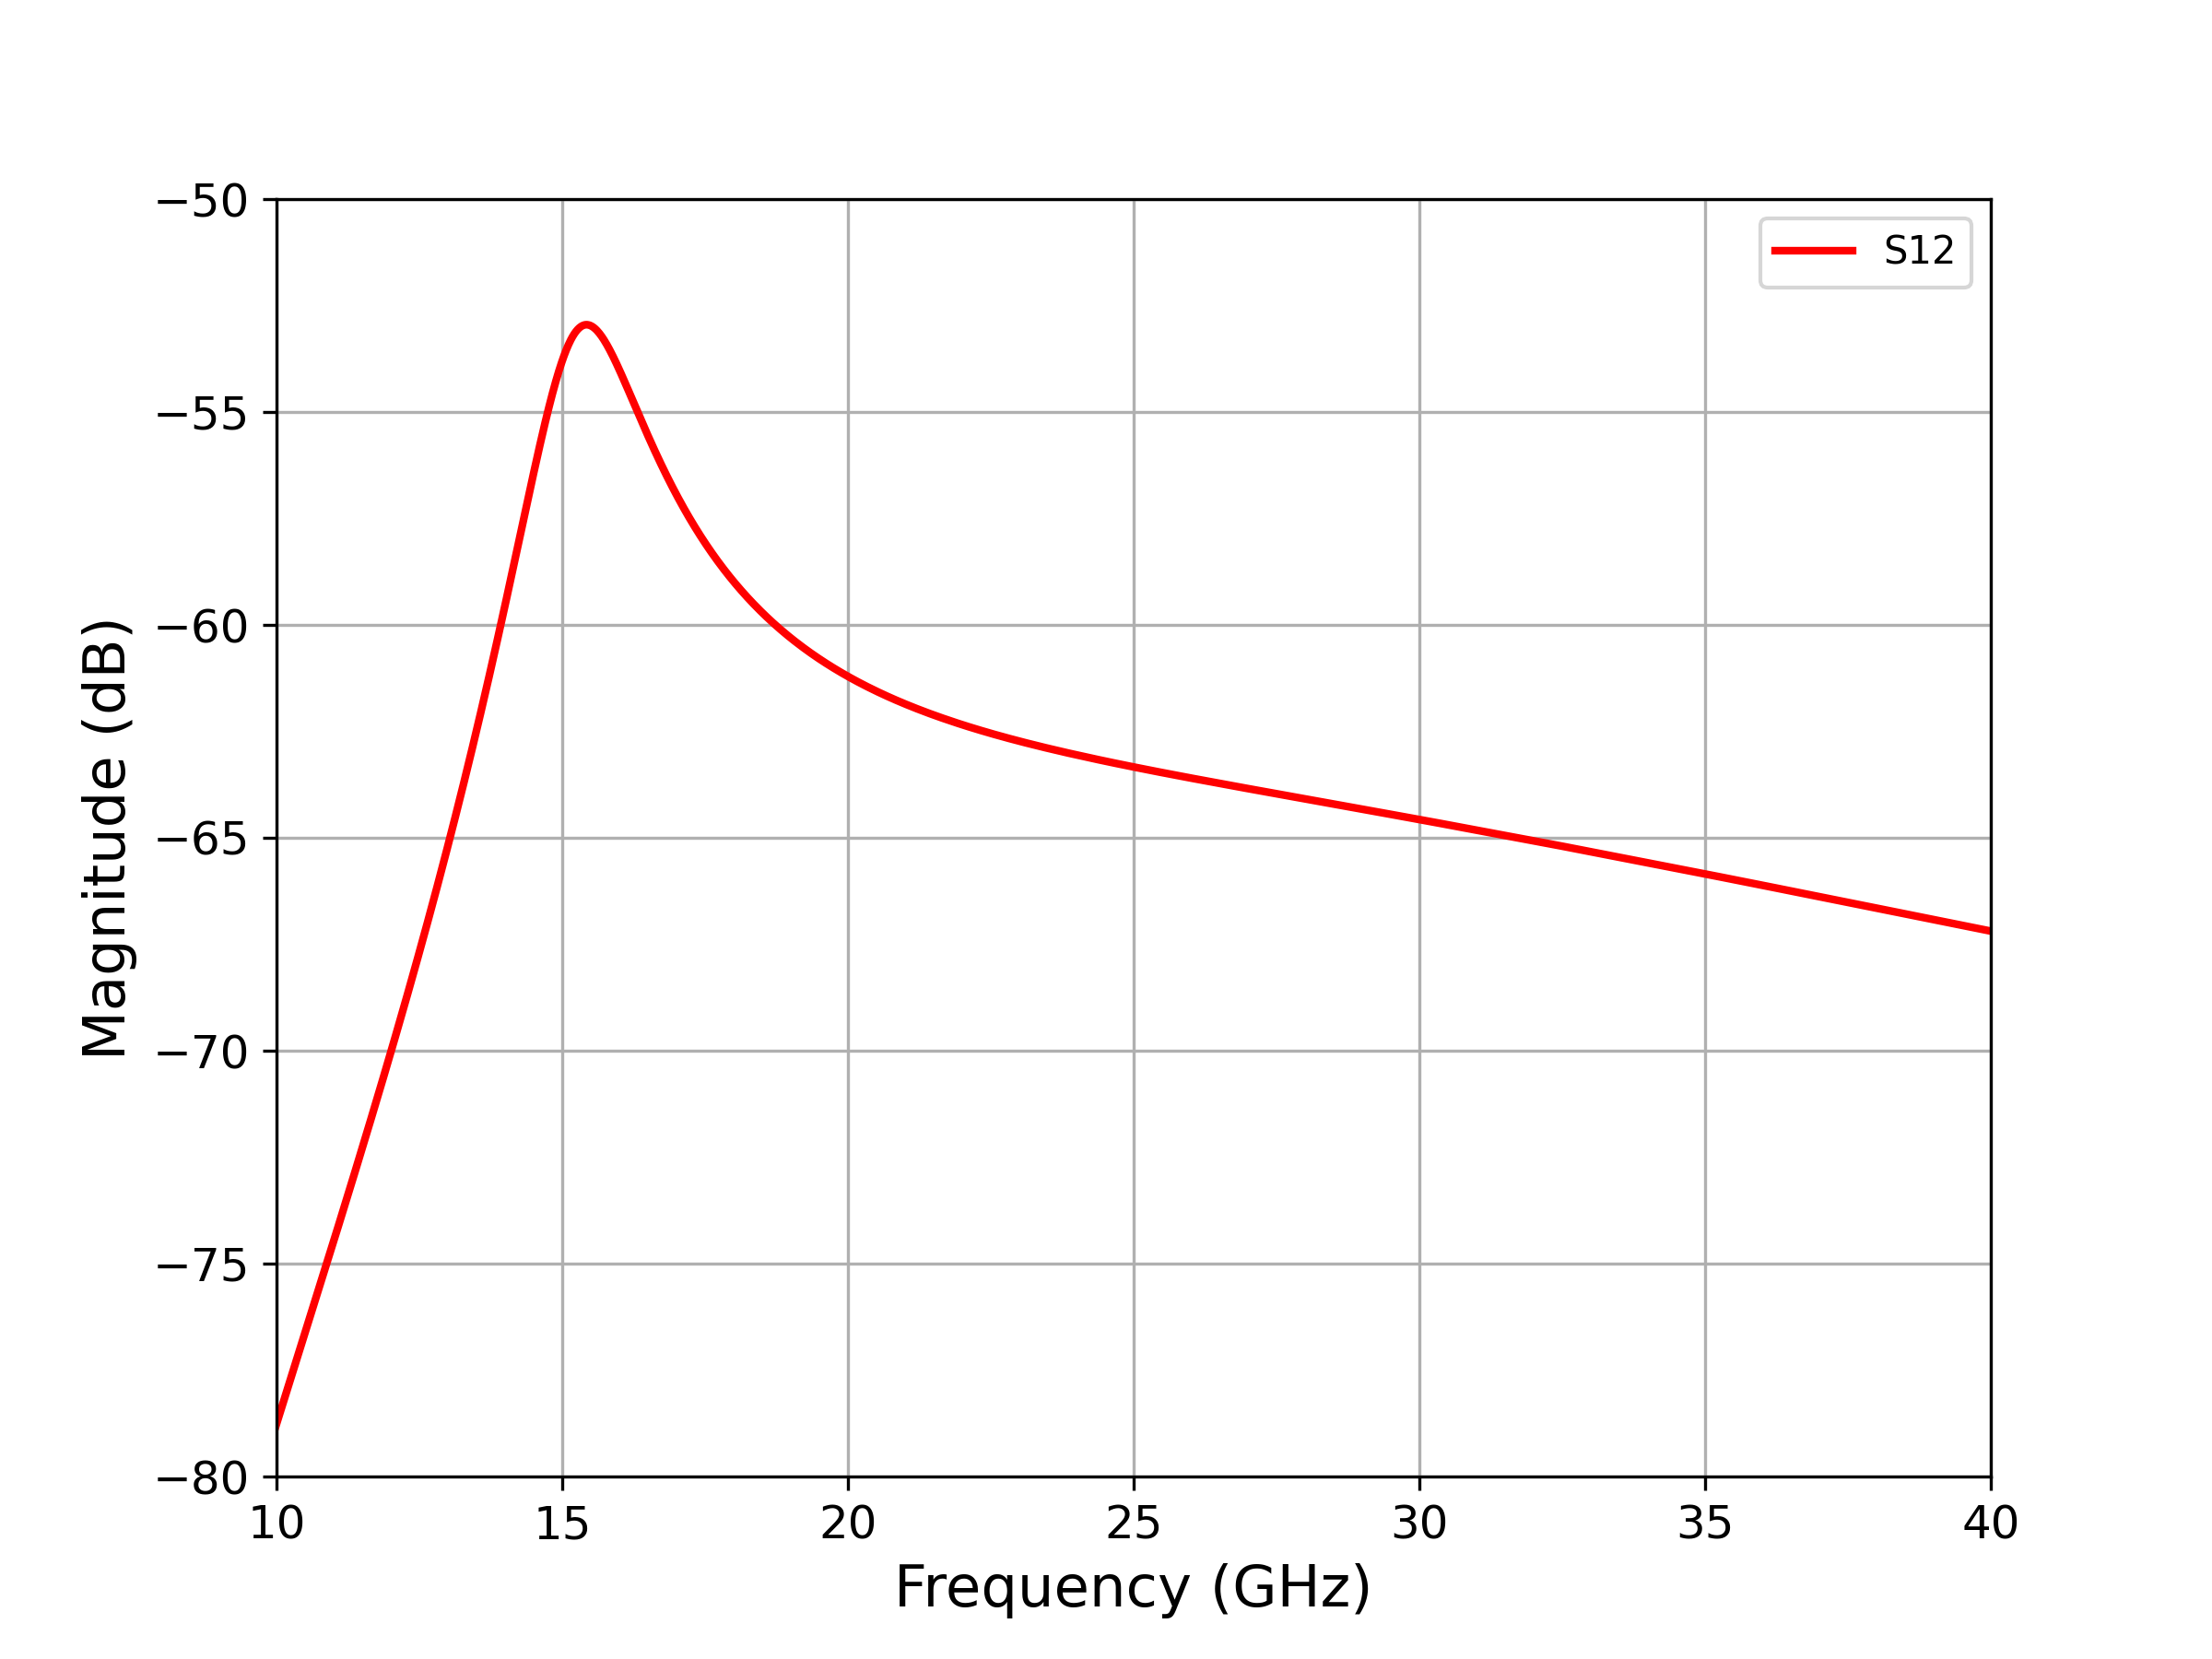
\includegraphics[width=\linewidth]{figures/two_stage_s12.png}
    \caption{}
     \label{fig:two-stage-without-cadence-s12}
  \end{subfigure}
  \caption{(a) $S_{11}$ parameter of a two-stage power amplifier (shown in Figure \ref{fig:double-stage-power-amplifier}) without matching network. (b) $S_{12}$ parameter of a two-stage power amplifier (shown in Figure \ref{fig:double-stage-power-amplifier}) without matching network.}
  \label{fig:two-stage-without-cadence-s11-s12}
\end{figure}

To increase gain and bandwidth, a second stage was introduced with the first stage. Now the value of $S_{11}$ is -1.5 dB at 15 GHz, which means the matching is improved compared with a single-stage power amplifier. The value of input return loss ($S_{12}$) is less than -50 dB throughout the BW.
% \begin{figure}[H]
%     \centering
%     \resizebox{0.8\textwidth}{!}{
%     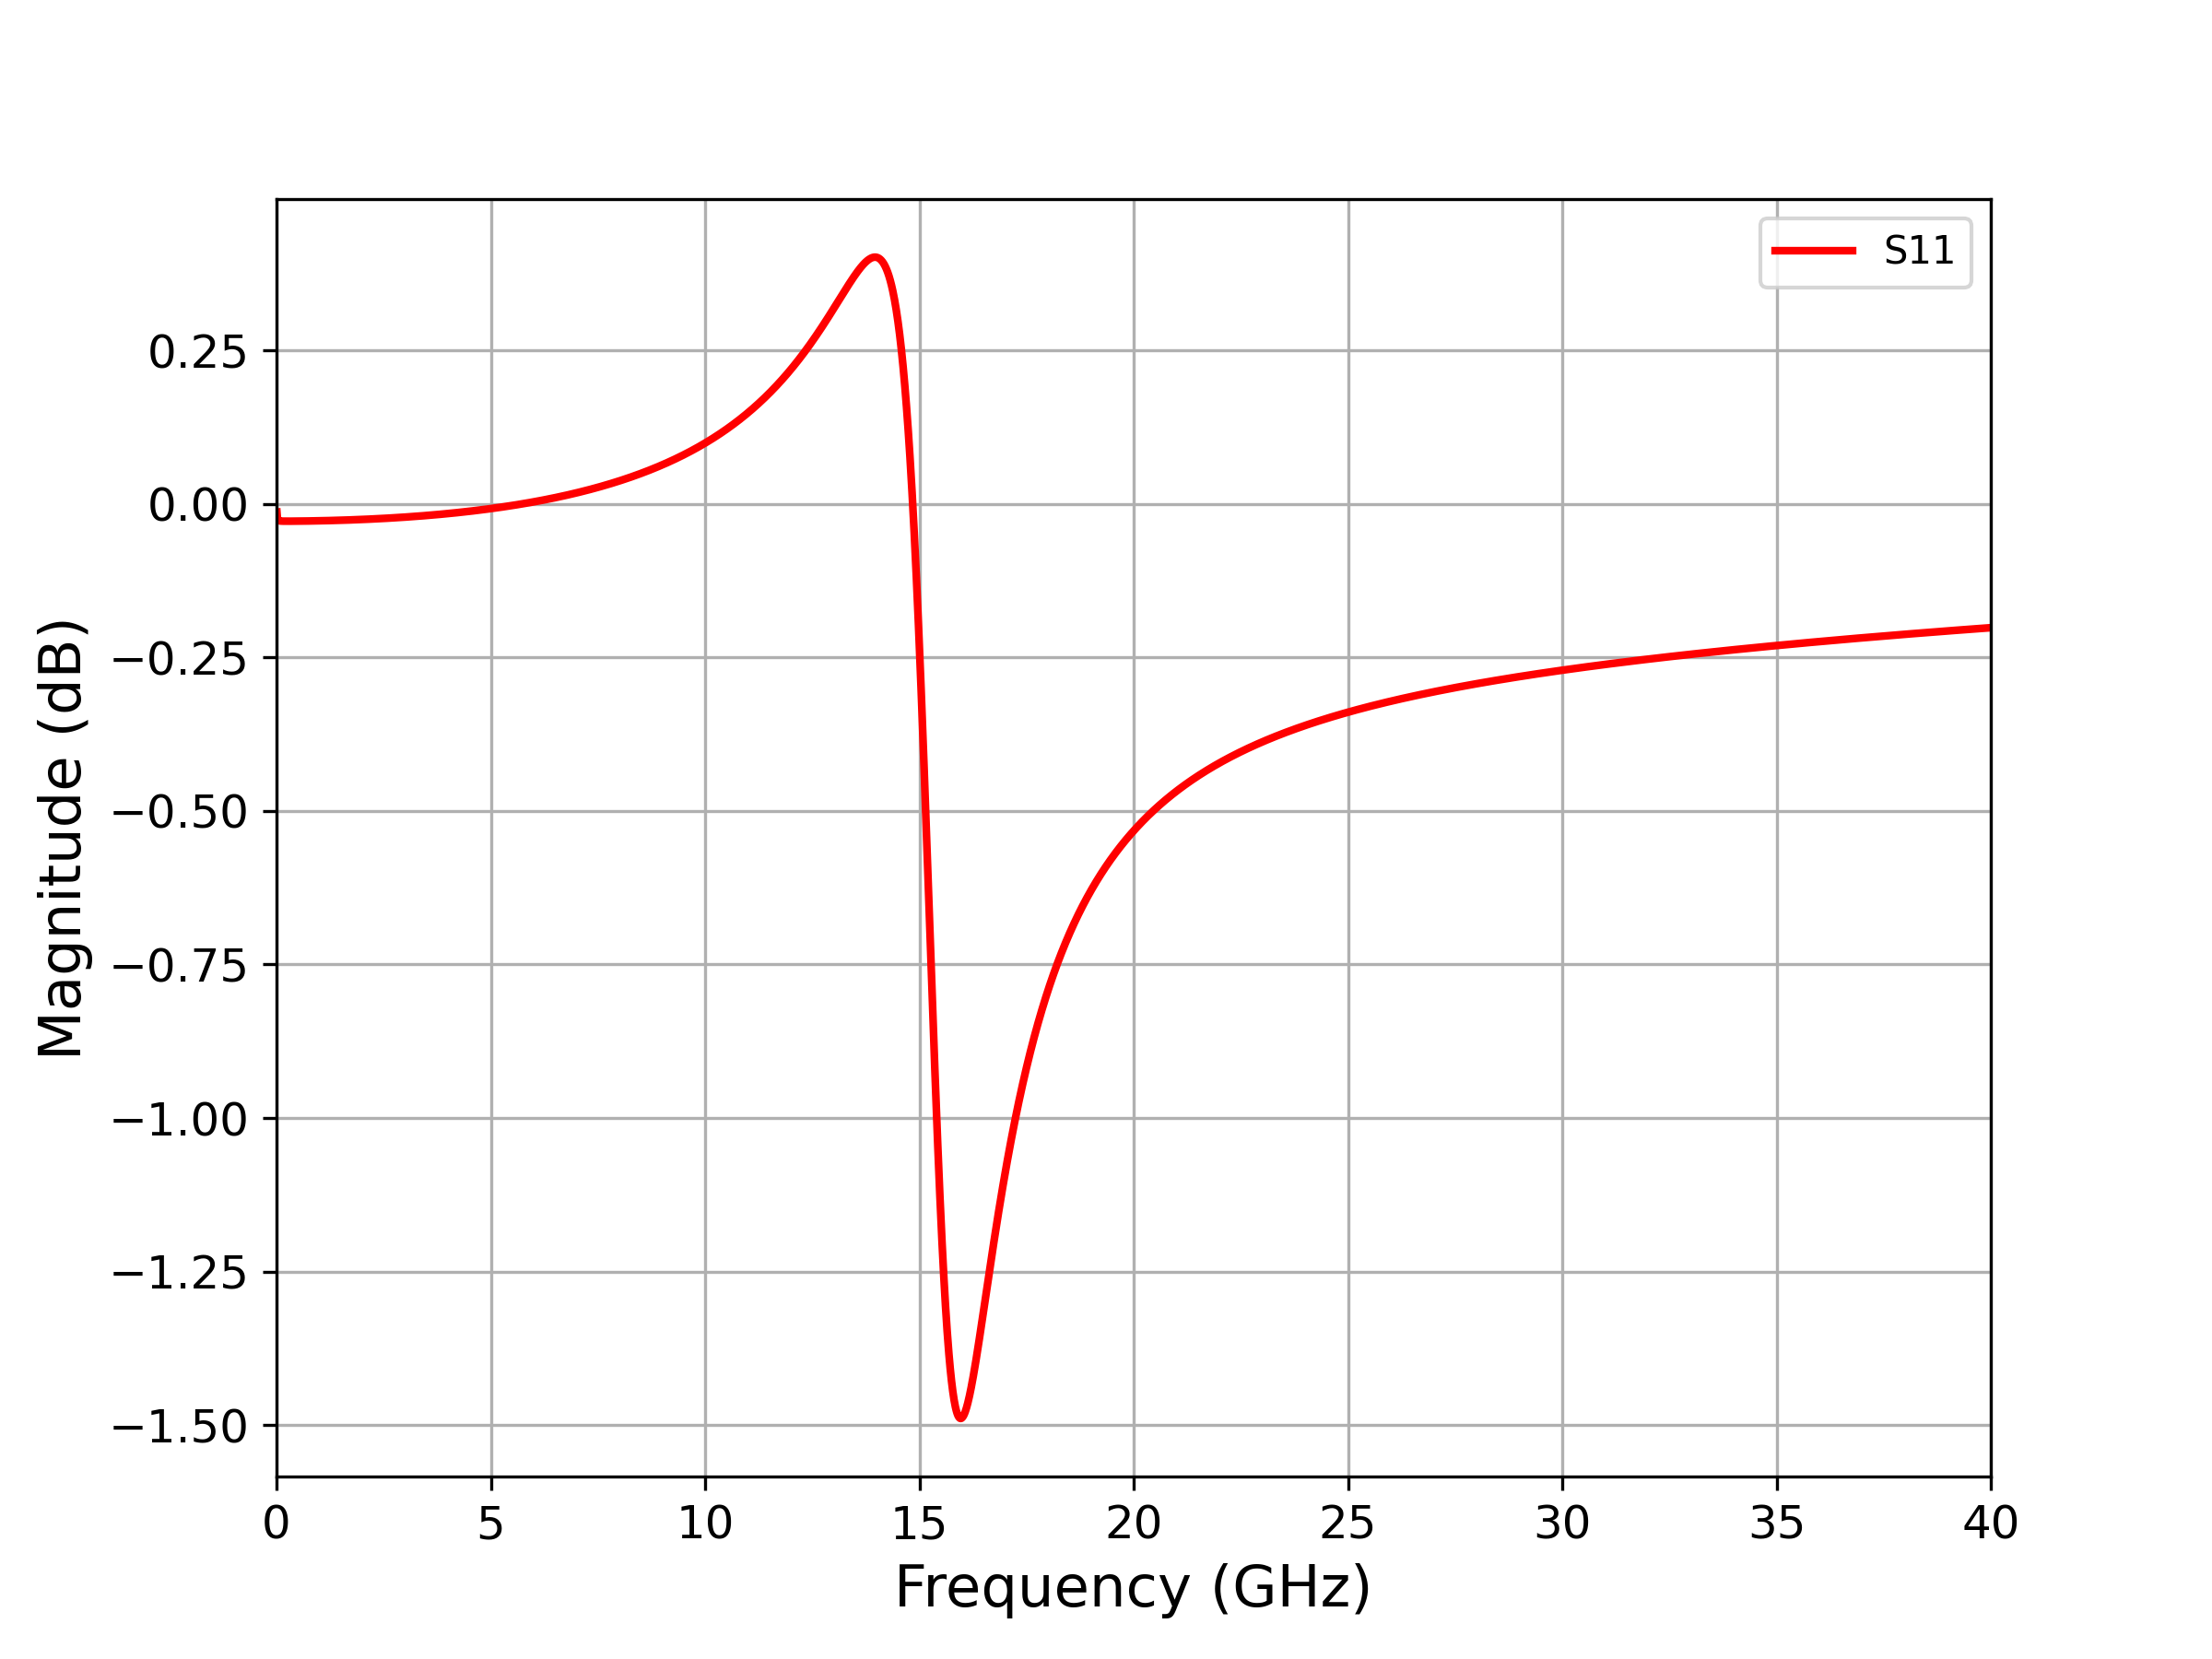
\includegraphics[]{figures/two_stage_s11.png}
%     }
%     \caption{$S_{11}$ parameter of a two-stage power amplifier (shown in Figure \ref{fig:double-stage-power-amplifier}) without matching network. The $S_{11}$ parameter is plotted from 0 GHz to 60 GHz.}
%     \label{fig:two-stage-without-cadence-s11}
% \end{figure}
% \begin{figure}[H]
%     \centering
%     \resizebox{0.8\textwidth}{!}{
%     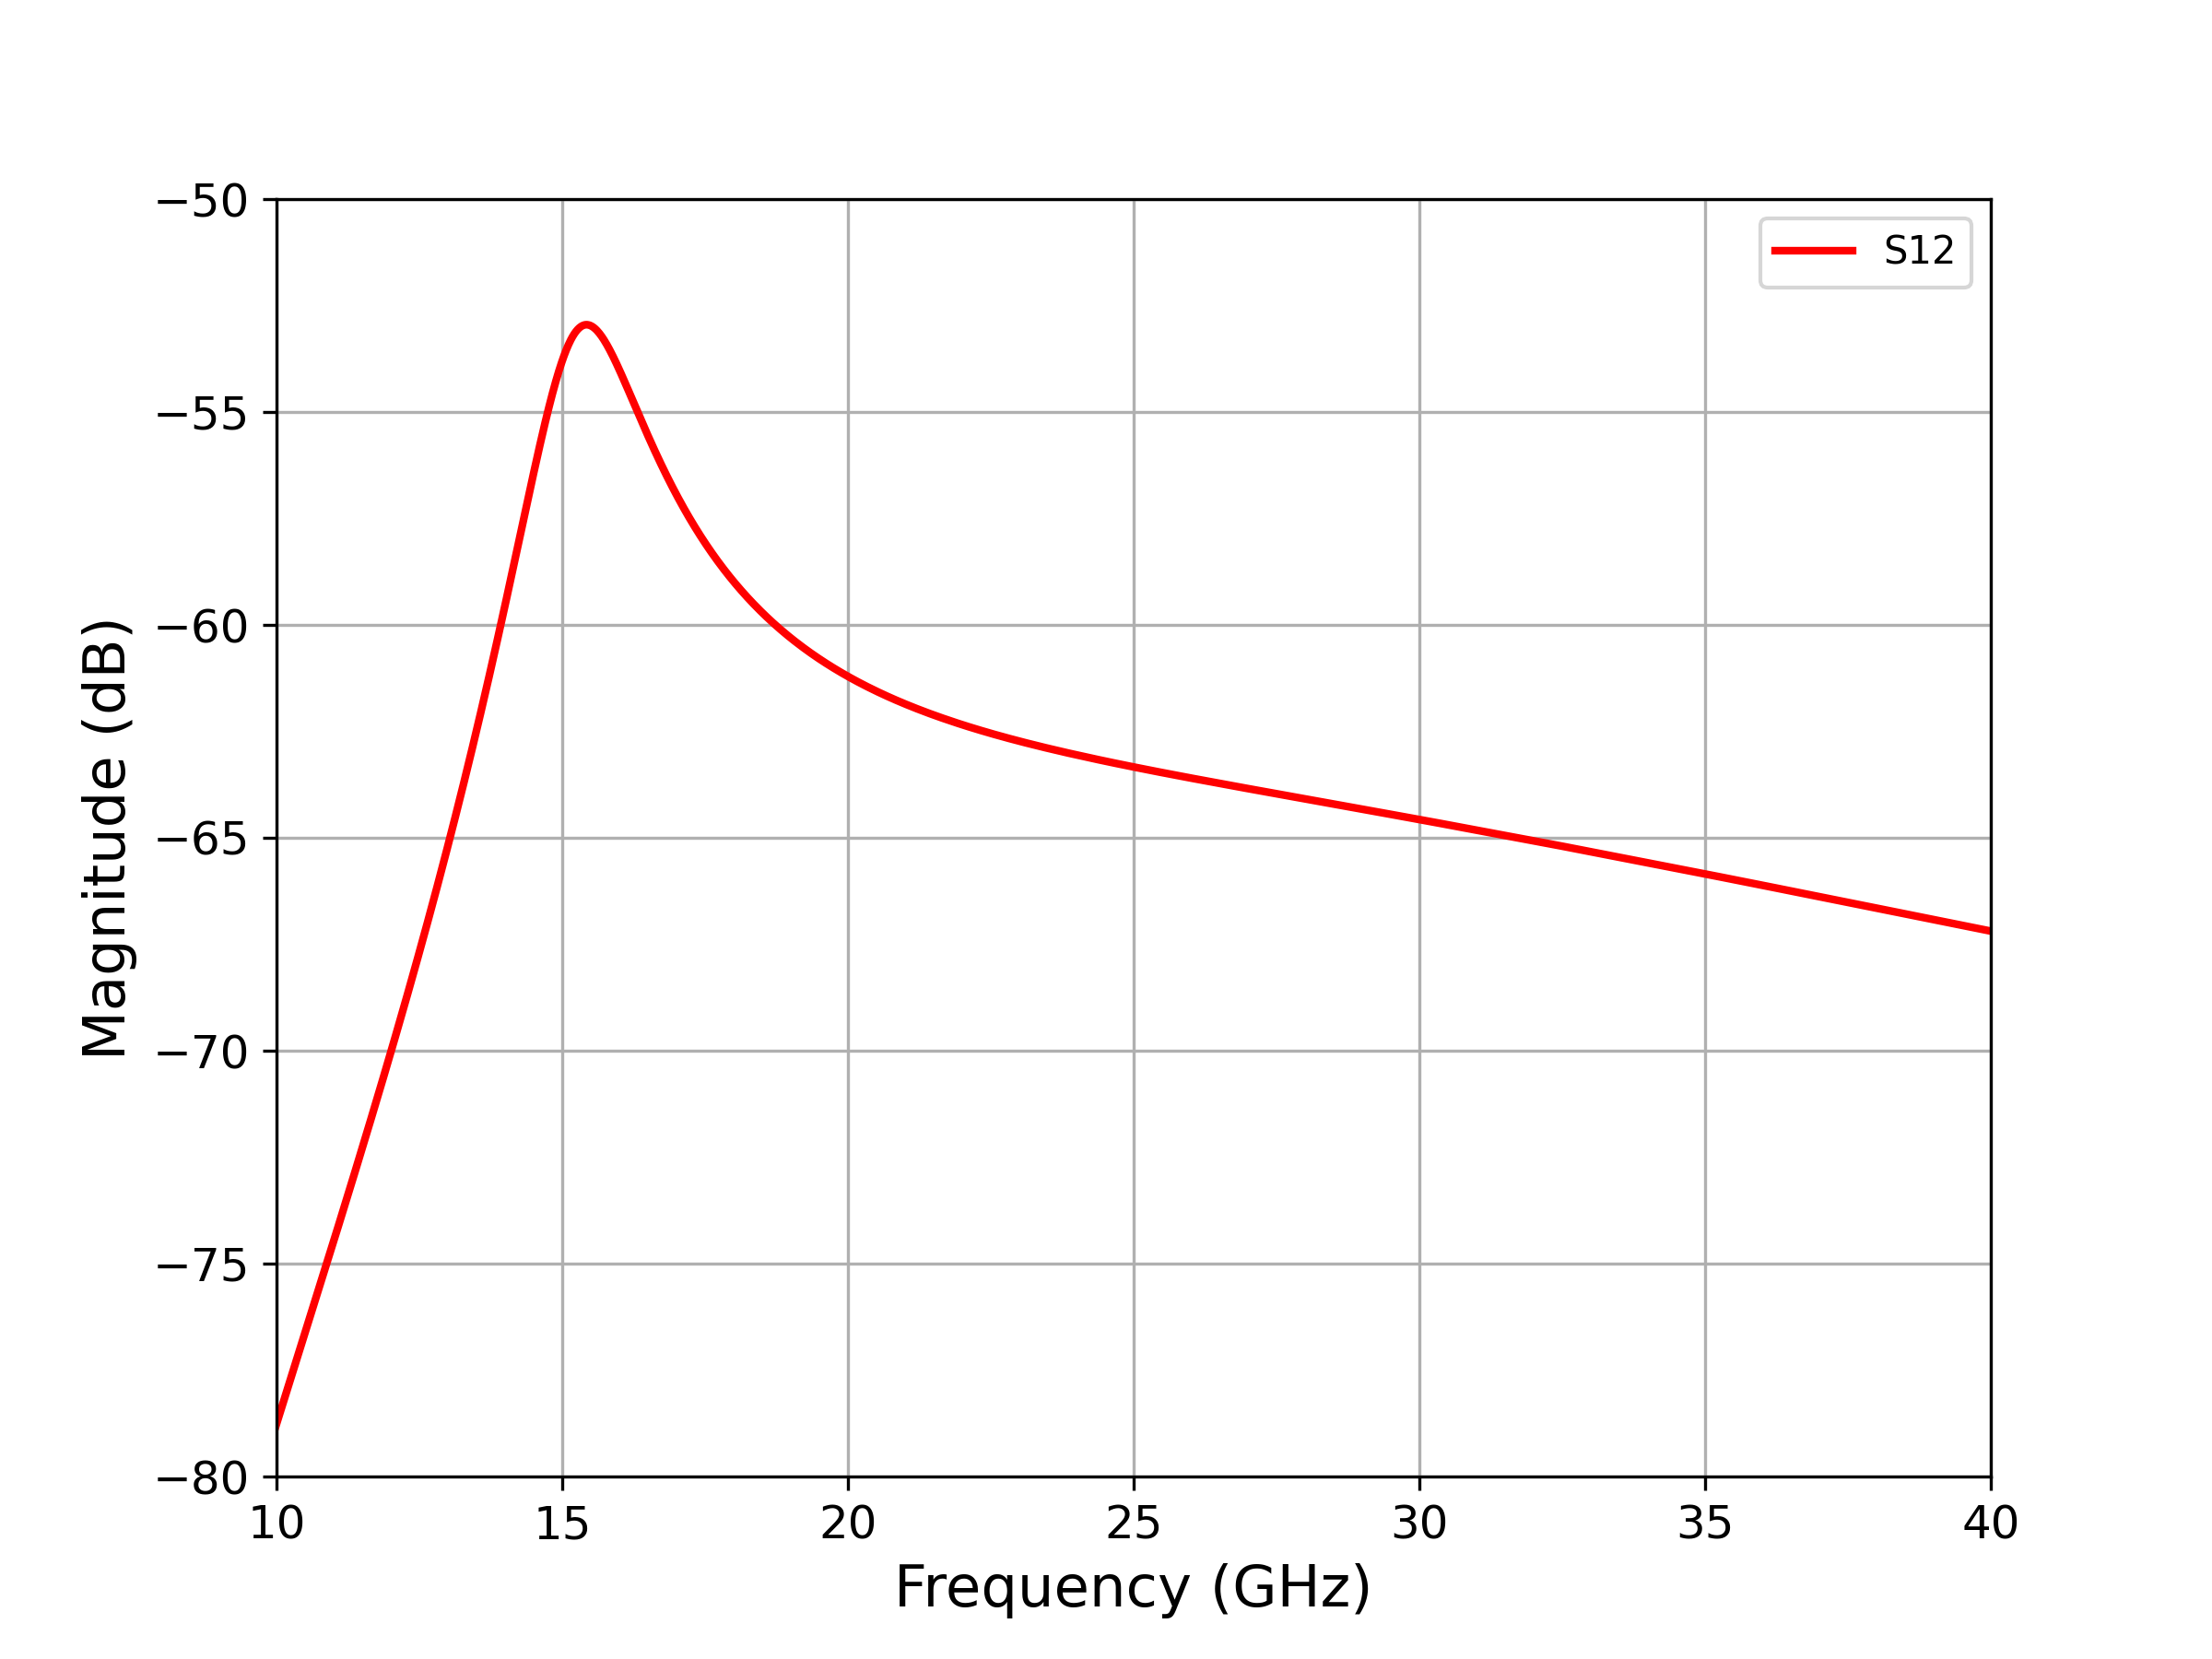
\includegraphics[]{figures/two_stage_s12.png}
%     }
%     \caption{$S_{12}$ parameter of a two-stage power amplifier (shown in Figure \ref{fig:double-stage-power-amplifier}) without matching network. The $S_{12}$ parameter is plotted from 0 GHz to 60 GHz.}
%     \label{fig:two-stage-without-cadence-s12}
% \end{figure}

\begin{figure}[H]
  \centering
  \begin{subfigure}{0.49\textwidth}
    \centering
    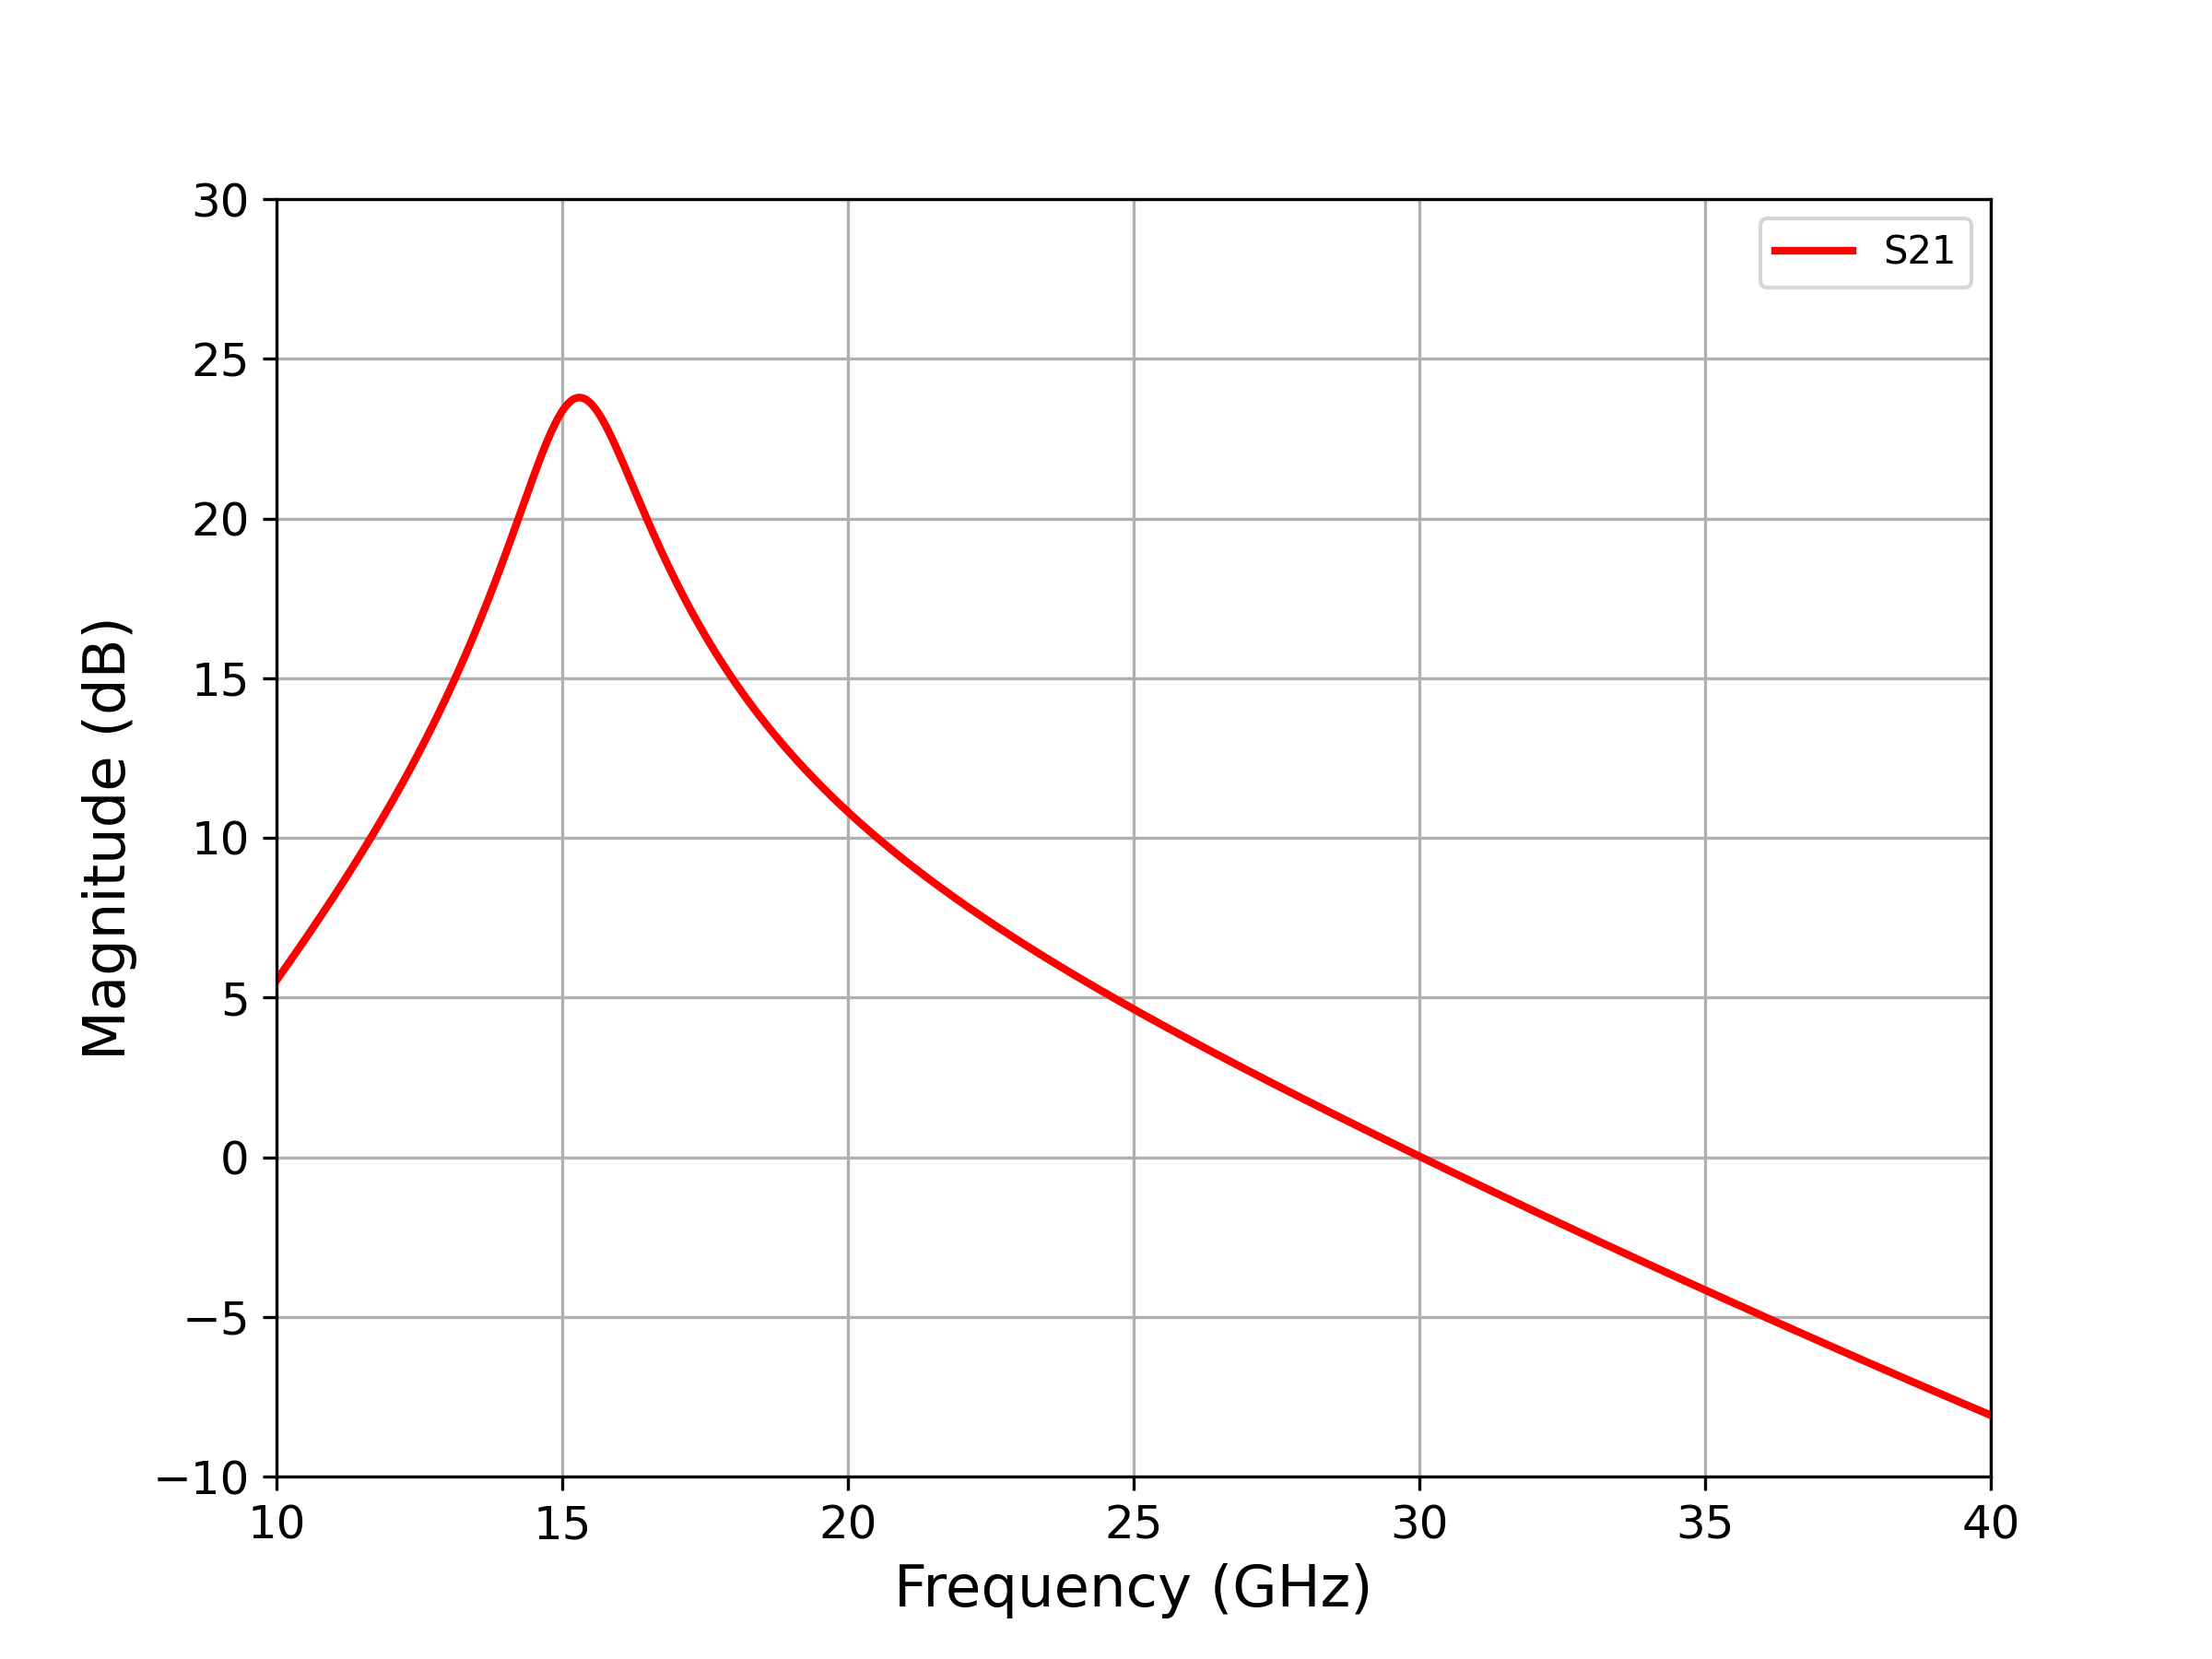
\includegraphics[width=\linewidth]{figures/two_stage_s21.png}
    \caption{}
    \label{fig:two-stage-without-cadence-s21}
  \end{subfigure}
  \hfill
  \begin{subfigure}{0.49\textwidth}
    \centering
    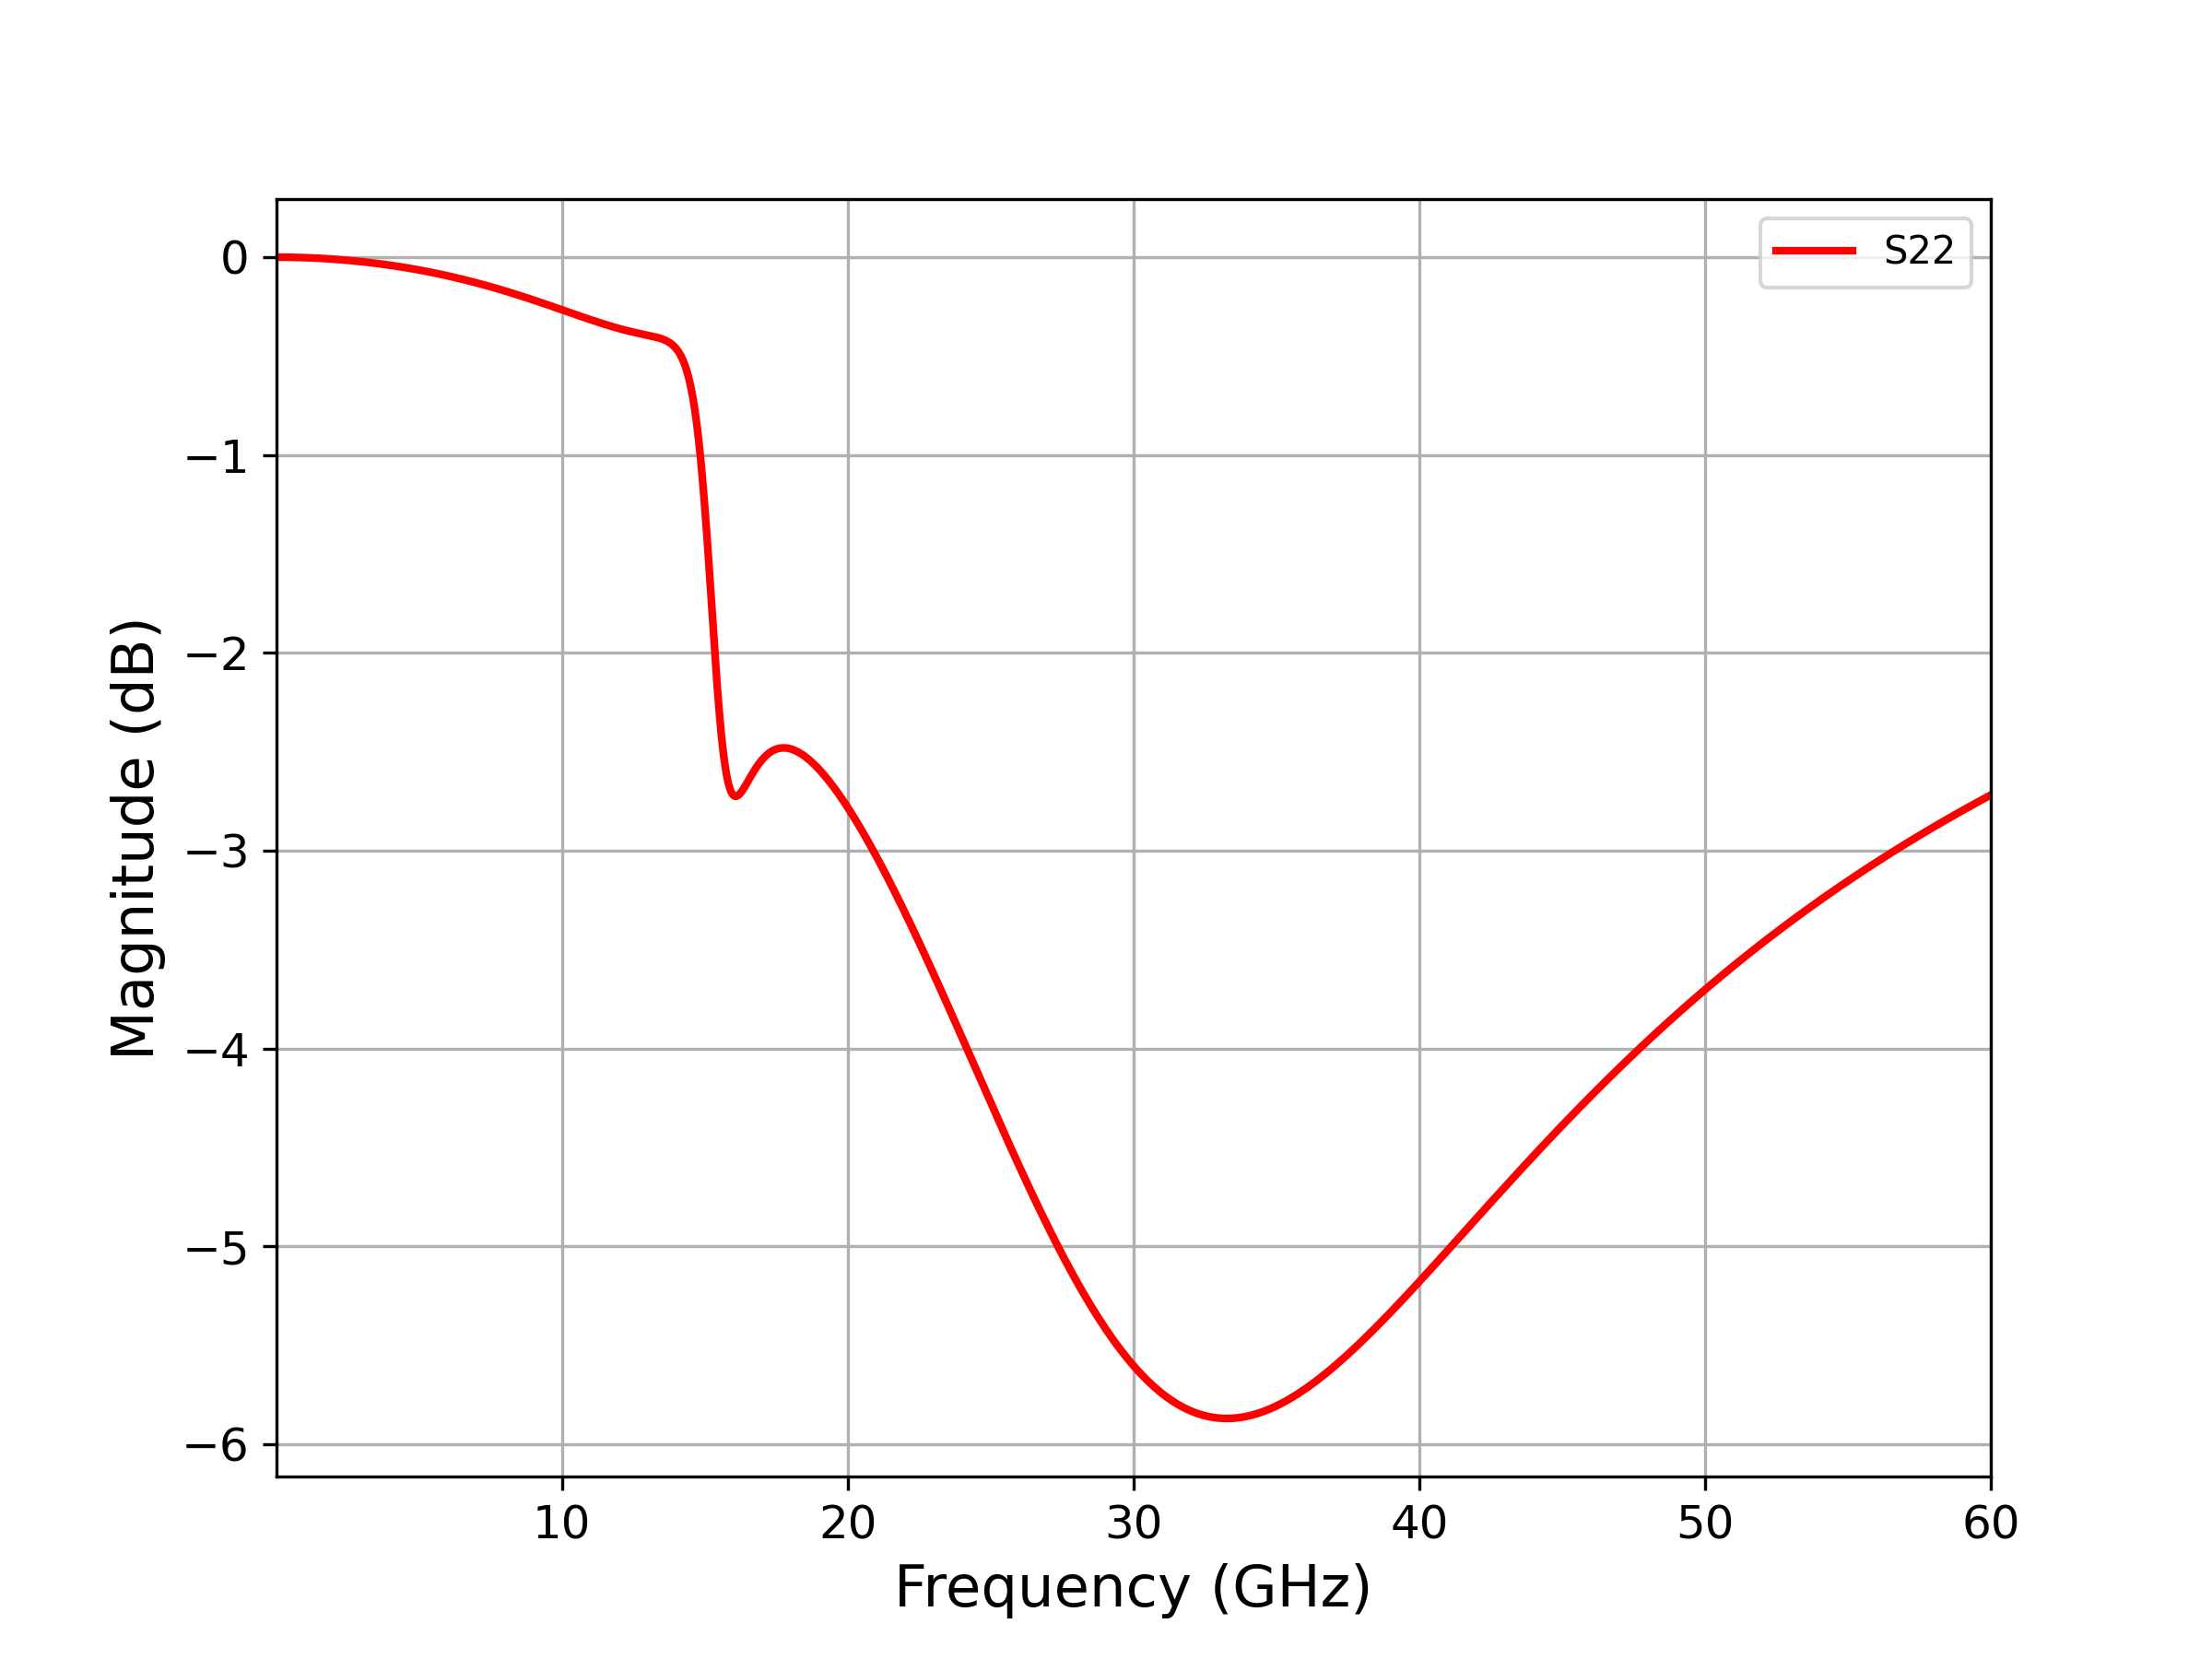
\includegraphics[width=\linewidth]{figures/two_stage_s22.png}
    \caption{}
     \label{fig:two-stage-without-cadence-s22}
  \end{subfigure}
  \caption{(a) $S_{21}$ parameter of a two-stage power amplifier (shown in Figure \ref{fig:double-stage-power-amplifier}) without matching network. (b) $S_{22}$ parameter of a two-stage power amplifier (shown in Figure \ref{fig:double-stage-power-amplifier}) without matching network.}
  \label{fig:two-stage-without-cadence-s21-s22}
\end{figure}

The maximum value of $S_{21}$ of a two-stage power amplifier is 24 dB at 15 GHz, which indicates a significant enhancement compared to the single-stage amplifier. However, the gain decreases drastically as the frequency increases, which limits the bandwidth, and the value of $S_{22}$ is less than -3 dB through 20 GHz to 50 GHz.
% \begin{figure}[H]
%     \centering
%     \resizebox{0.8\textwidth}{!}{
%     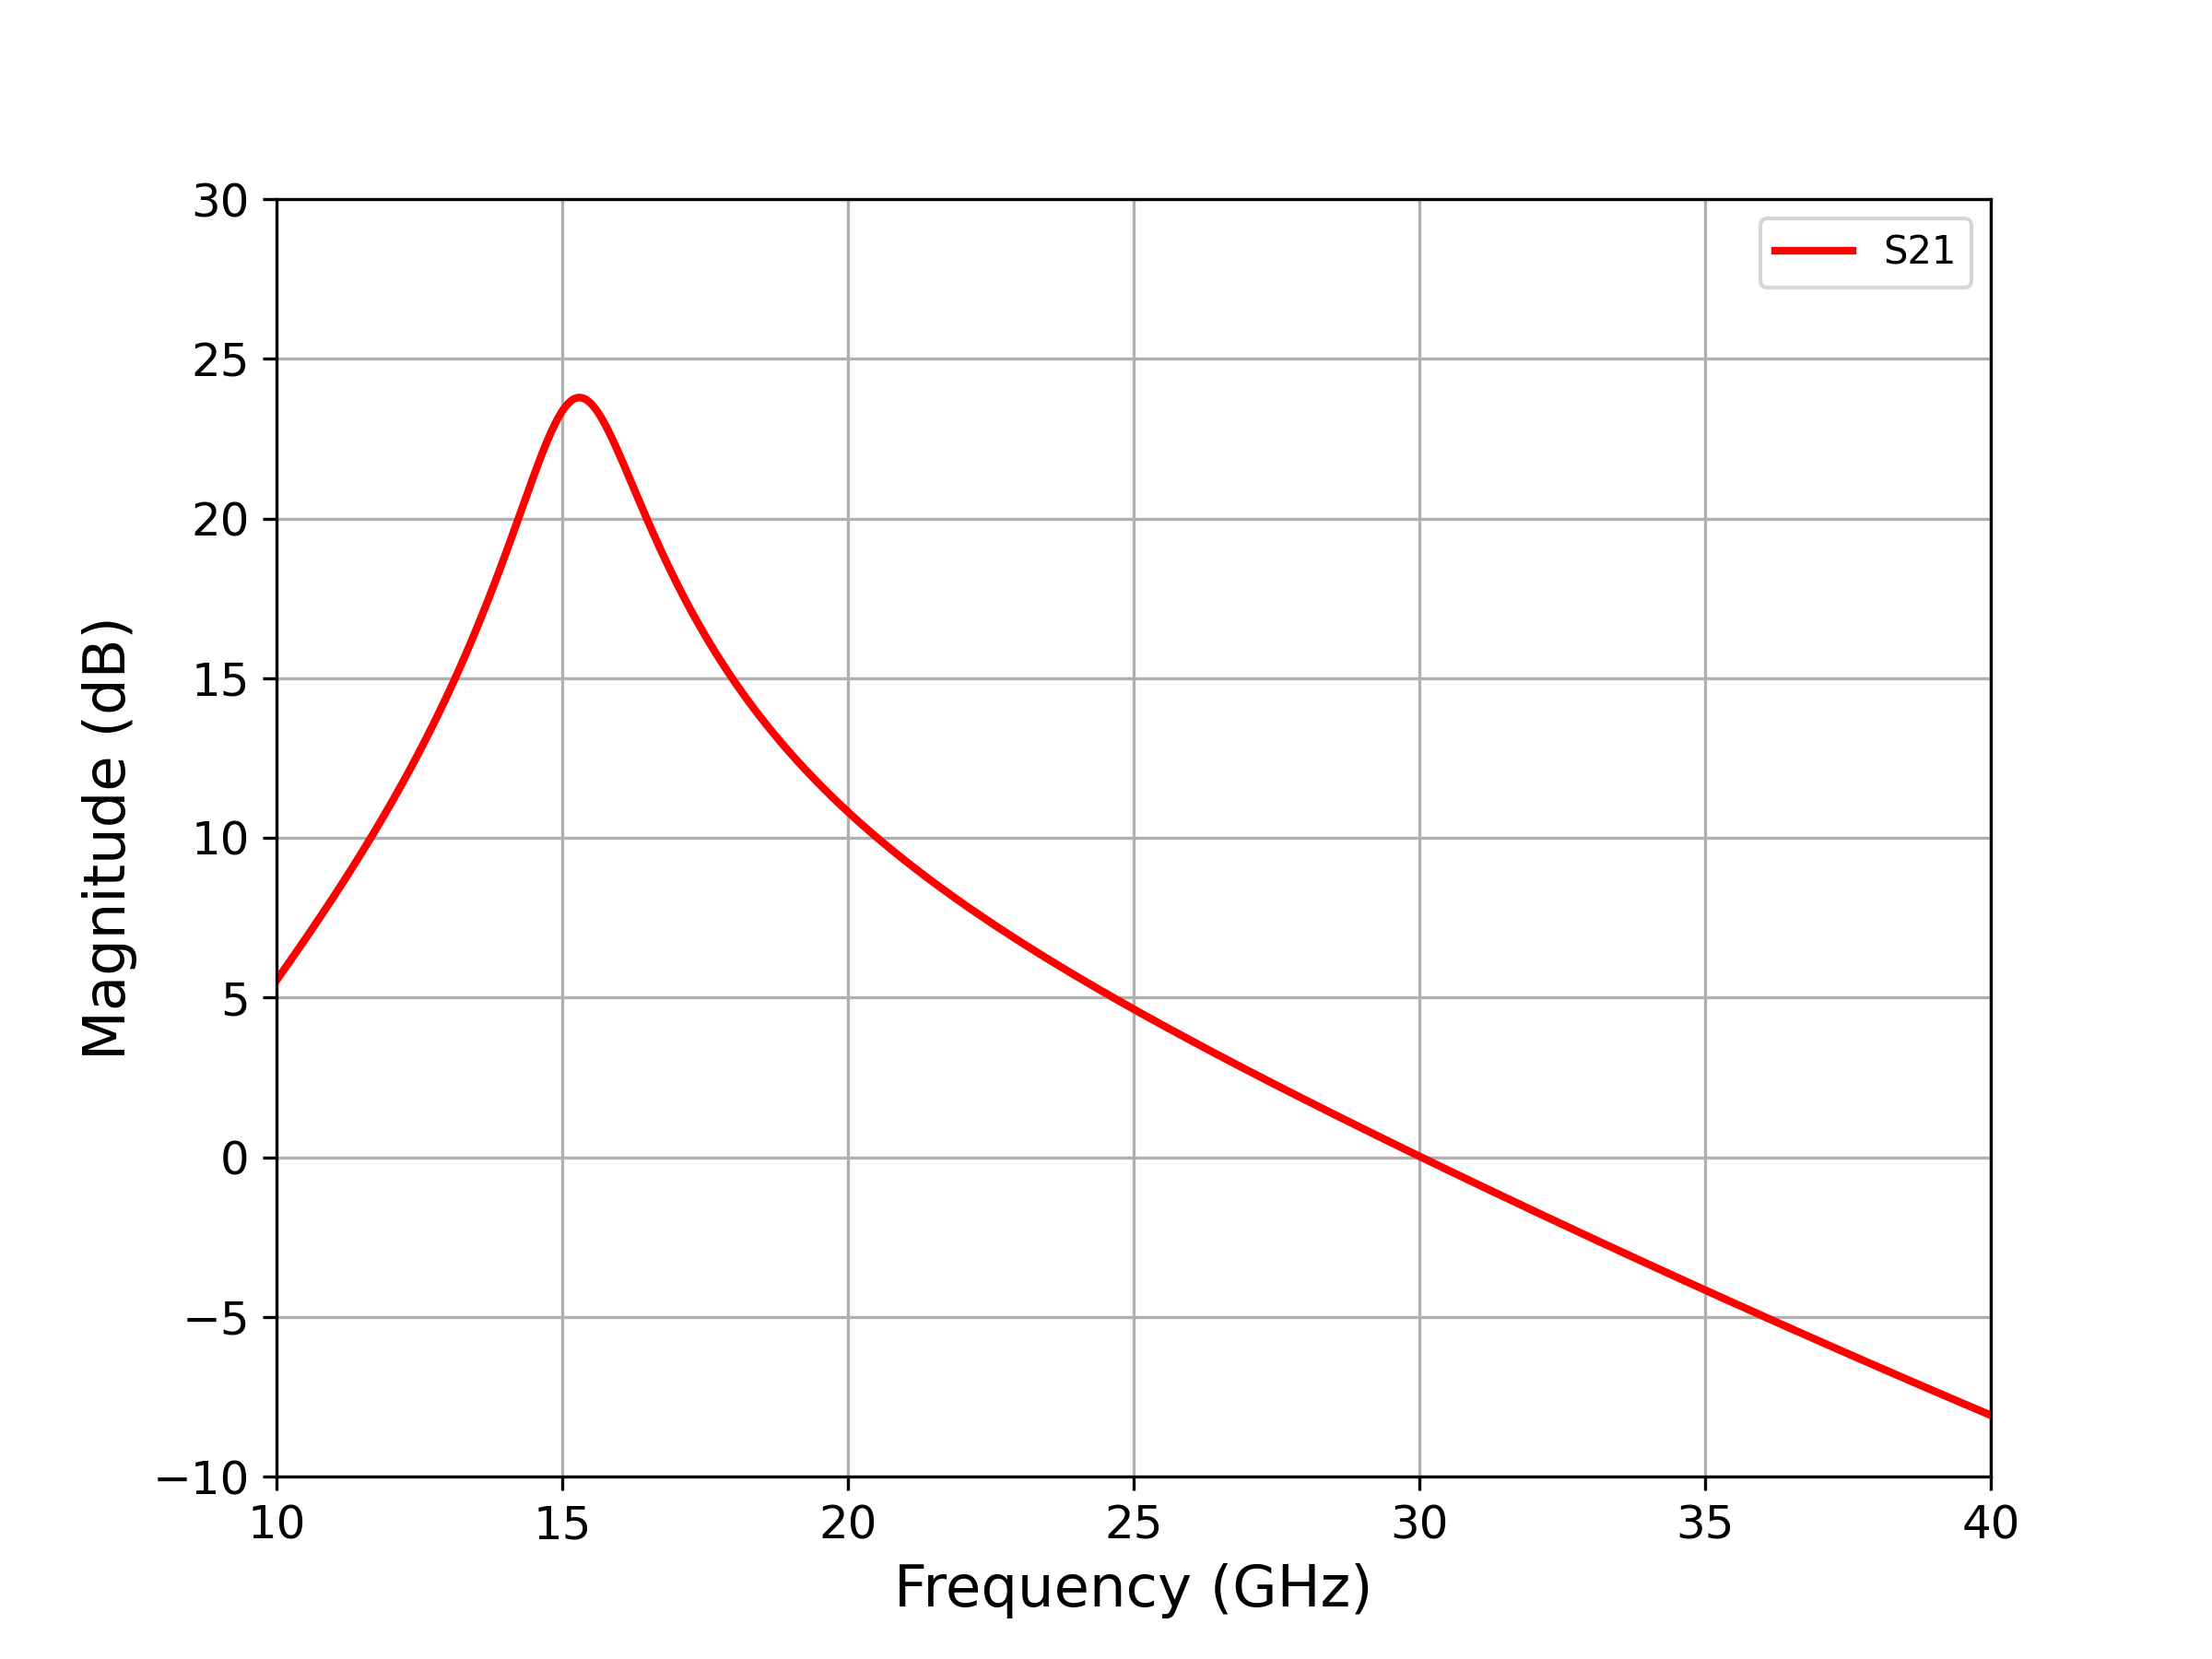
\includegraphics[]{figures/two_stage_s21.png}
%     }
%     \caption{$S_{21}$ parameter of a two-stage power amplifier (shown in Figure \ref{fig:double-stage-power-amplifier}) without matching network. The $S_{21}$ parameter is plotted from 0 GHz to 60 GHz.}
%     \label{fig:two-stage-without-cadence-s21}
% \end{figure}
% \begin{figure}[H]
%     \centering
%     \resizebox{0.8\textwidth}{!}{
%     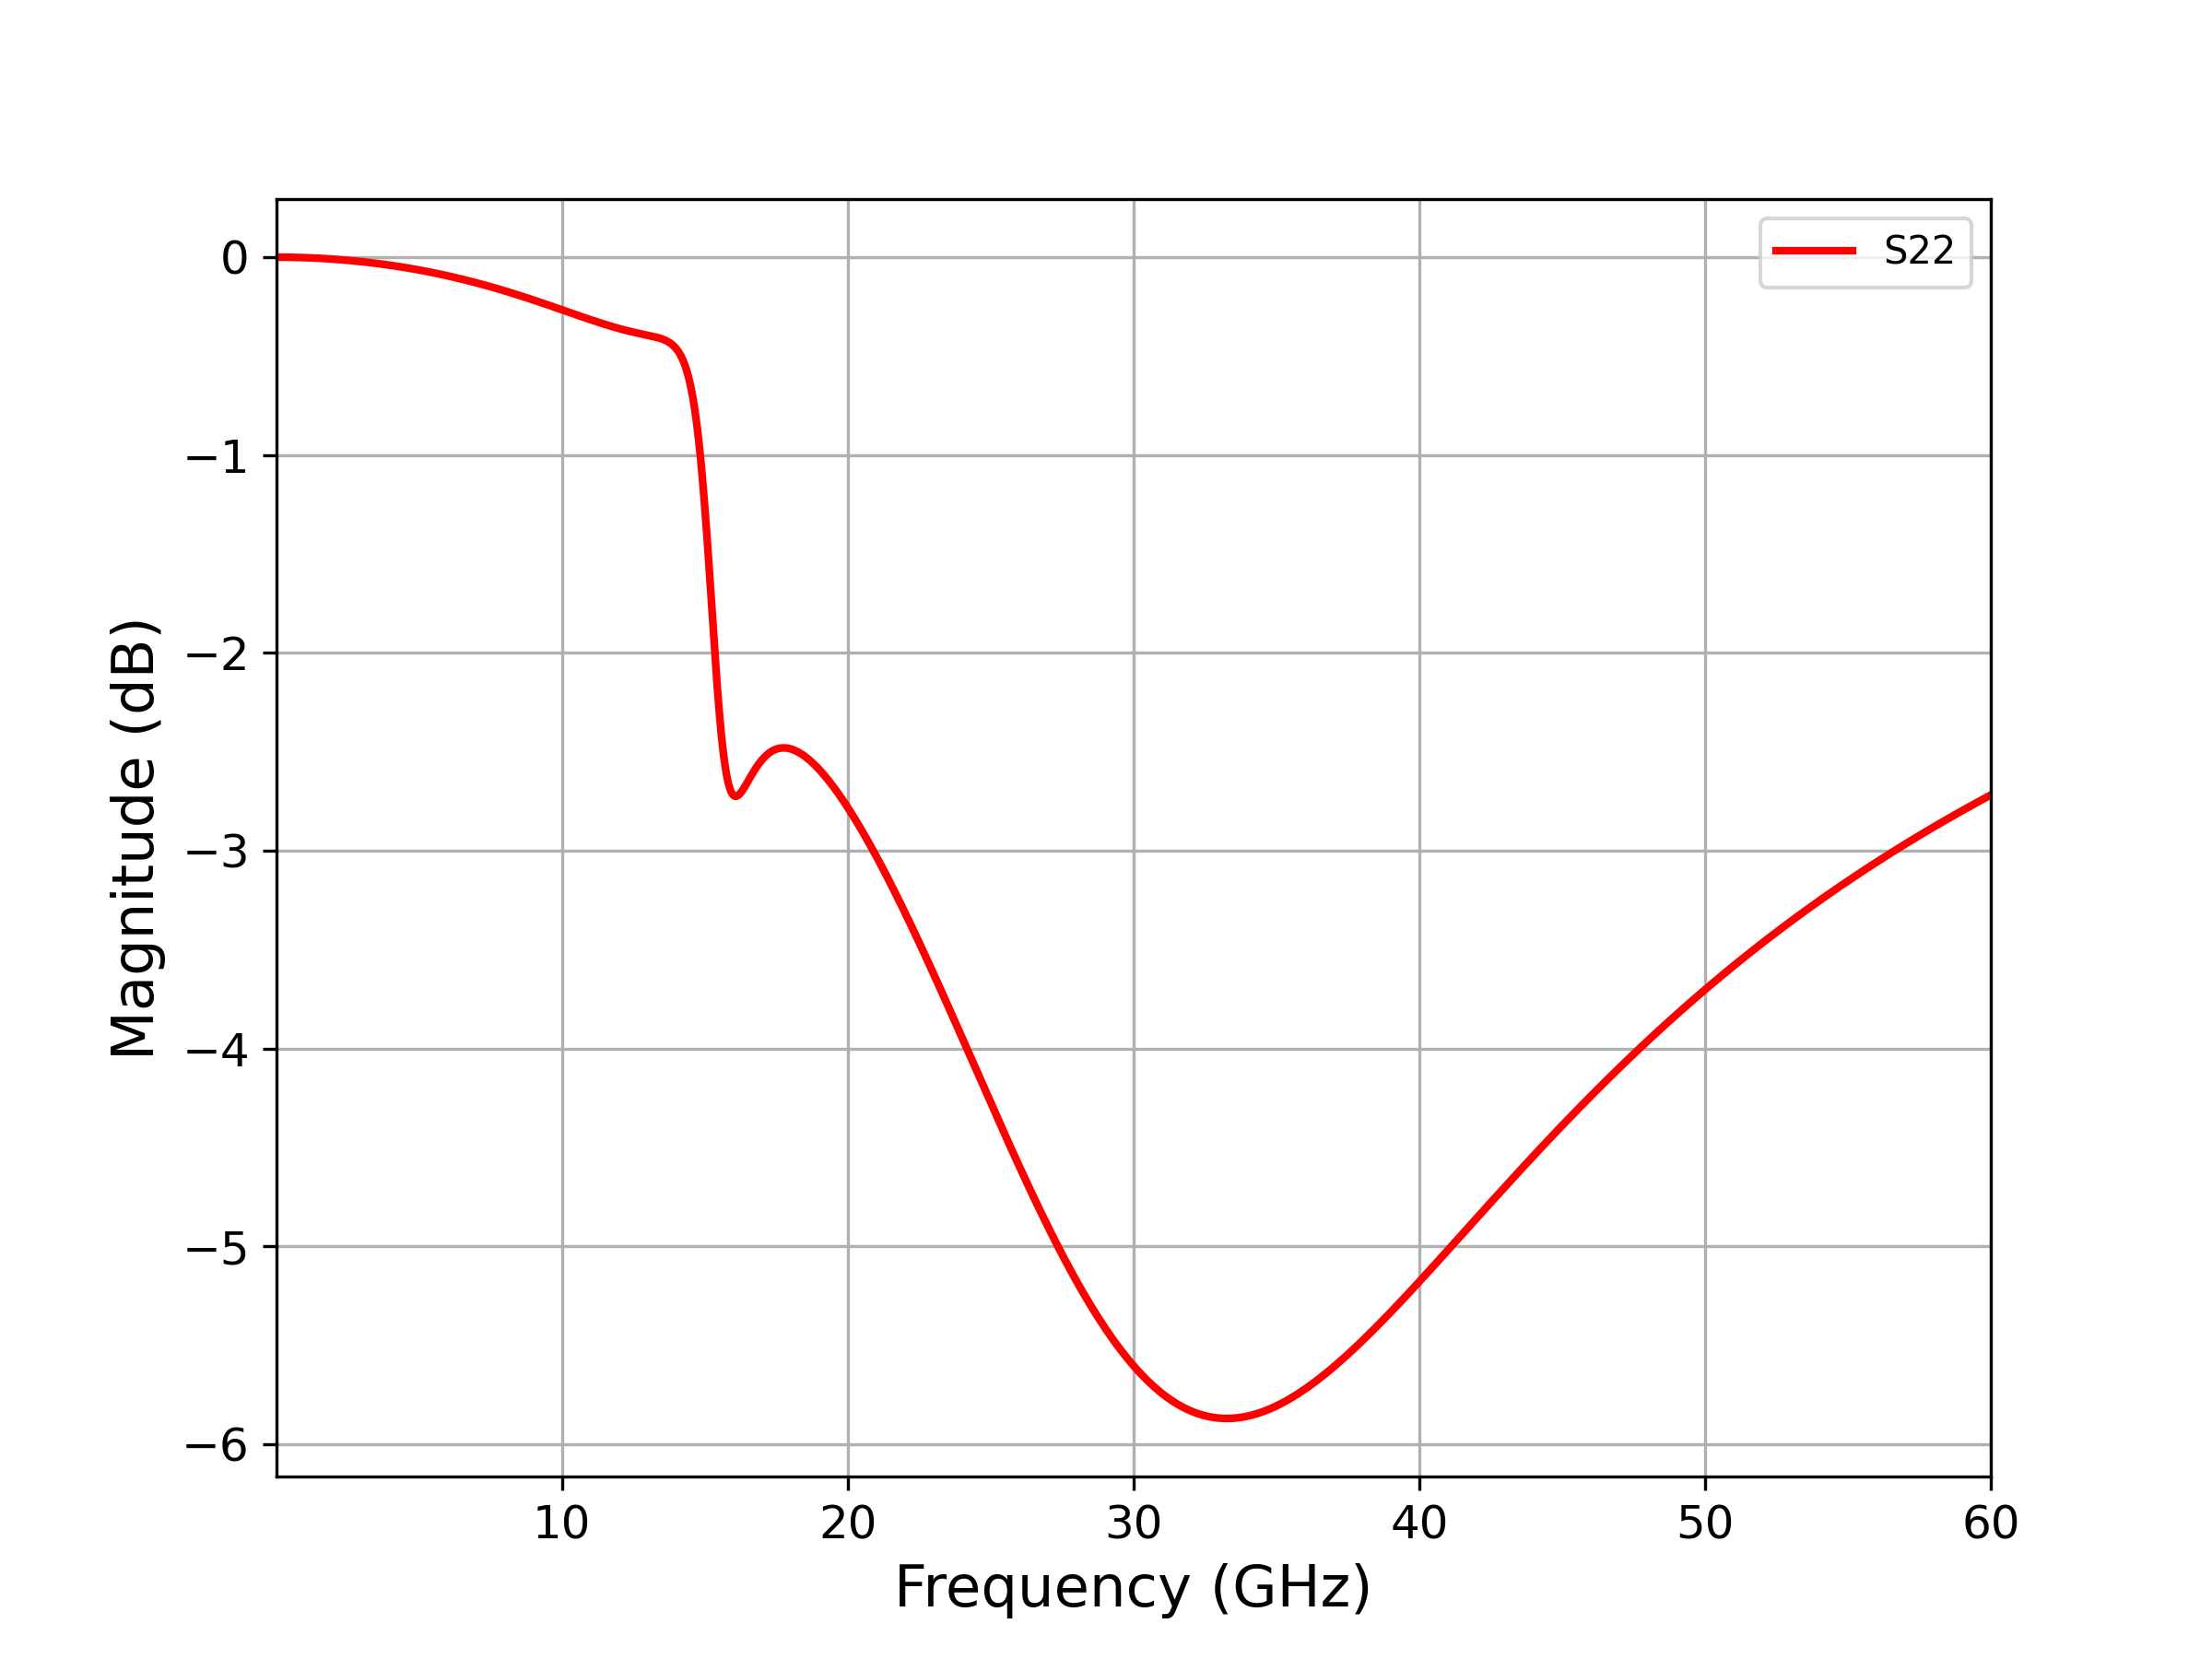
\includegraphics[]{figures/two_stage_s22.png}
%     }
%     \caption{$S_{22}$ parameter of a two-stage power amplifier (shown in Figure \ref{fig:double-stage-power-amplifier}) without matching network. The $S_{22}$ parameter is plotted from 0 GHz to 60 GHz.}
%     \label{fig:two-stage-without-cadence-s22}
% \end{figure}
%The $S$ parameter simulation of proposed two stage power amplifier(Figure \ref{fig:two-stage-with-input-interstage-matching}) with input and interstage matching network is shown below

\begin{figure}[H]
  \centering
  \begin{subfigure}{0.49\textwidth}
    \centering
    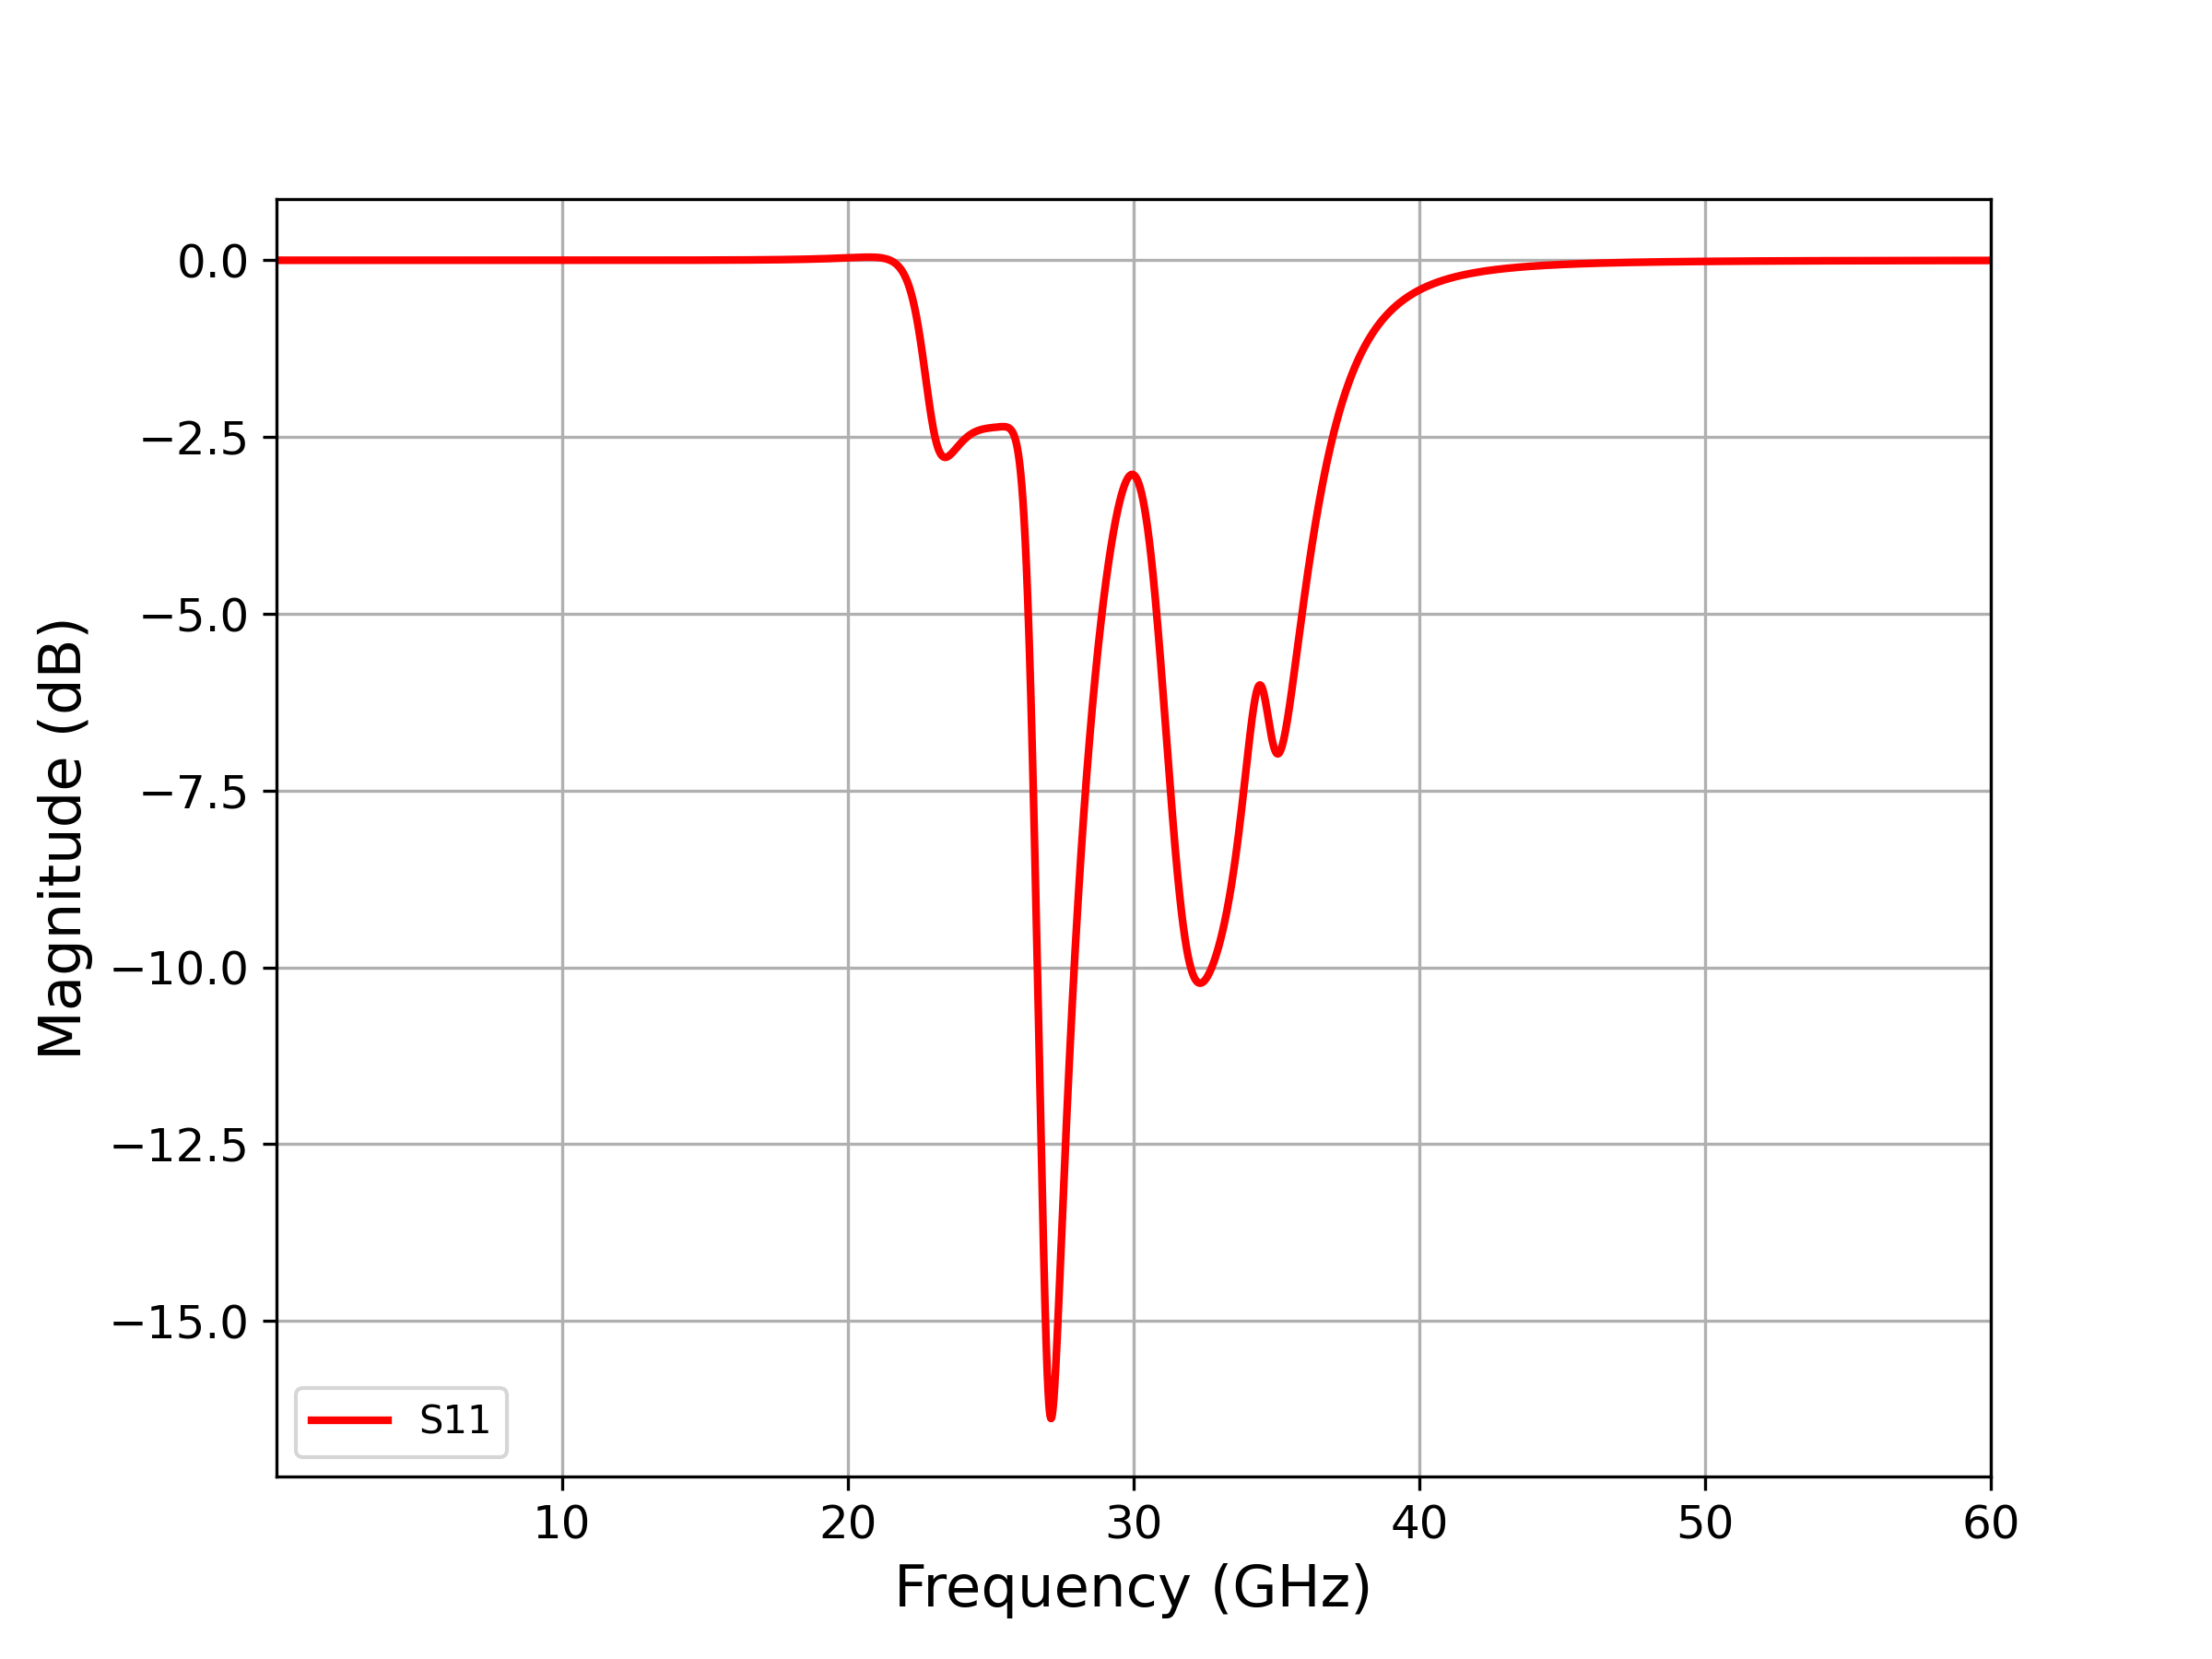
\includegraphics[width=\linewidth]{figures/two_stage_withMatching_s11.png}
    \caption{}
    \label{fig:two-stage-withmatching-cadence-s11}
  \end{subfigure}
  \hfill
  \begin{subfigure}{0.49\textwidth}
    \centering
    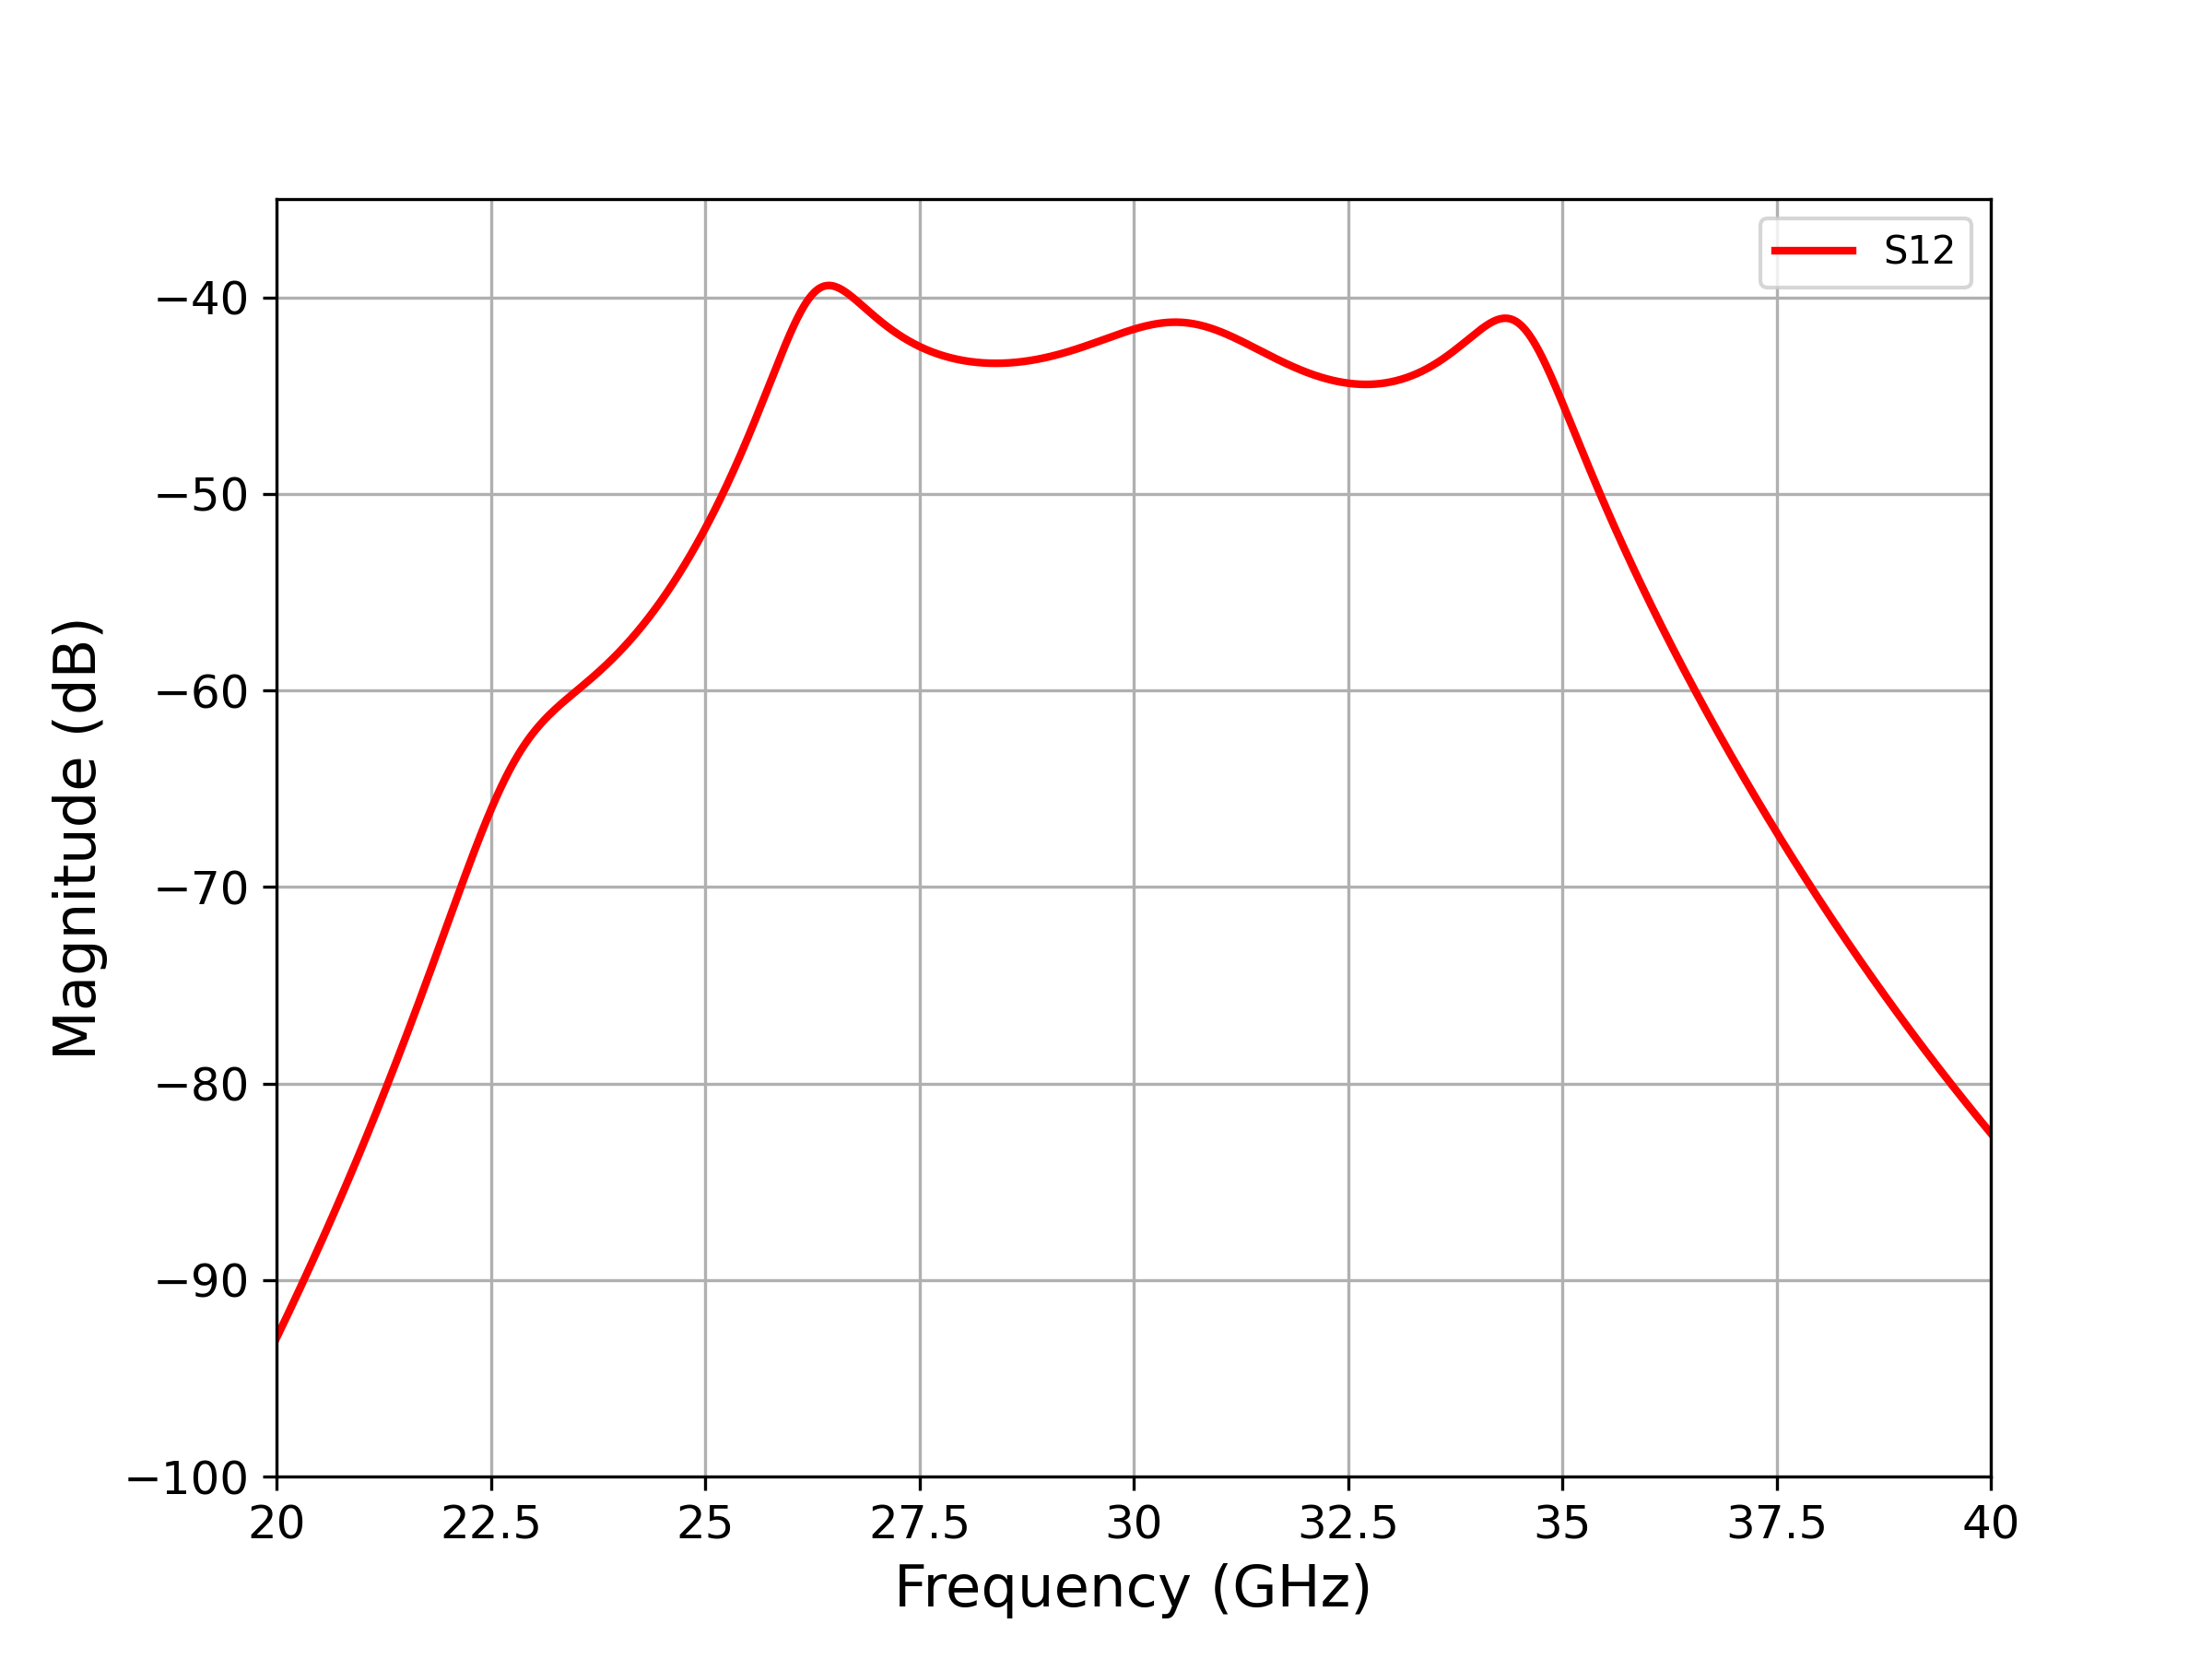
\includegraphics[width=\linewidth]{figures/two_stage_withMatching_s12.png}
    \caption{}
     \label{fig:two-stage-withmatching-cadence-s12}
  \end{subfigure}
  \caption{(a) $S_{11}$ parameter of a two-stage power amplifier (shown in Figure \ref{fig:two-stage-with-input-interstage-matching}) with input and interstage matching network. (b) $S_{12}$ parameter of a two-stage power amplifier (shown in Figure \ref{fig:two-stage-with-input-interstage-matching}) with input and interstage matching network.}
  \label{fig:two-stage-withmatching-cadence-s11-s12}
\end{figure}

To improve input impedance matching and inter-stage impedance matching, an input matching network is introduced at the input side of the proposed PA, and an inter-stage matching network is also introduced between the first and second stages of the proposed PA. The proposed PA network achieves better input matching with $S_{11}$ values of -16.38 dB at 27.12 GHz and -10.22 dB at 32.33 GHz. This indicates that a larger portion of the power is being absorbed by the amplifier rather than being reflected back. The proposed PA also exhibits good reverse isolation ($S_{12}$) of -40 dB over the frequency range of 25 to 35 GHz.

% \begin{figure}[H]
%     \centering
%     \resizebox{0.8\textwidth}{!}{
%     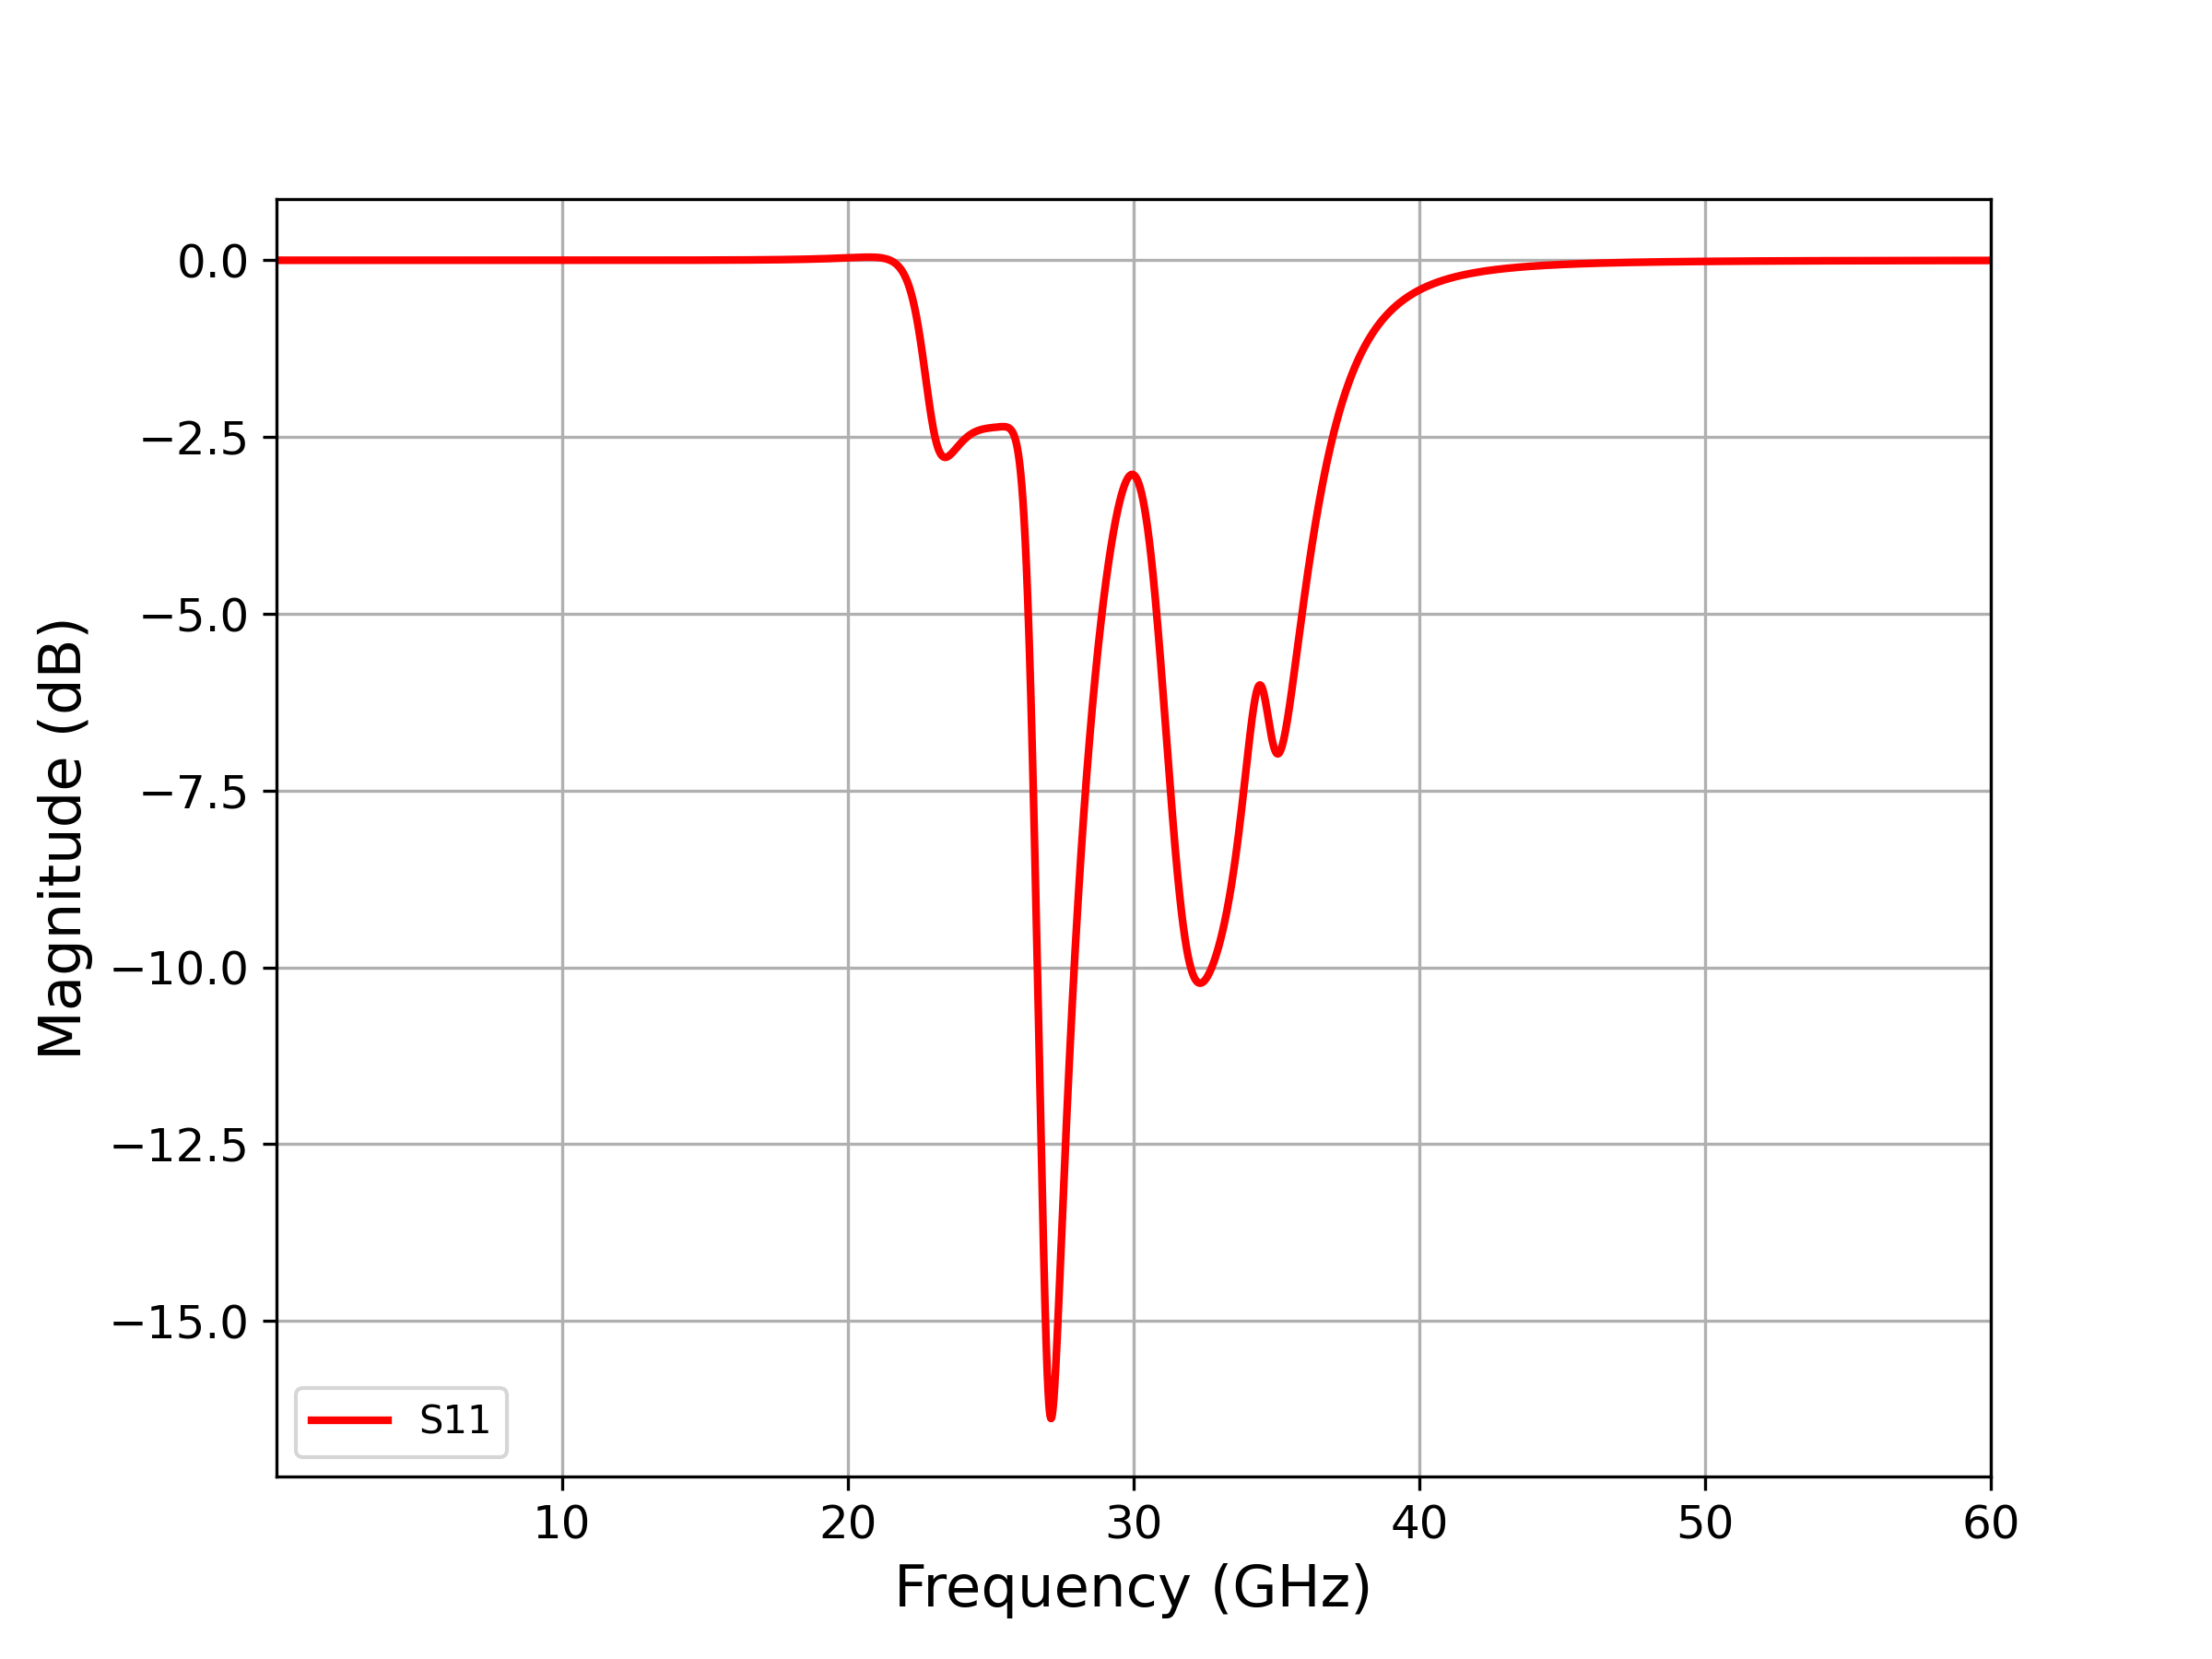
\includegraphics[]{figures/two_stage_withMatching_s11.png}
%     }
%     \caption{$S_{11}$ parameter of a two-stage power amplifier (shown in Figure \ref{fig:two-stage-with-input-interstage-matching}) with input and interstage matching network. The $S_{11}$ parameter is plotted from 0 GHz to 60 GHz.}
%     \label{fig:two-stage-withmatching-cadence-s11}
% \end{figure}
% \begin{figure}[H]
%     \centering
%     \resizebox{0.8\textwidth}{!}{
%     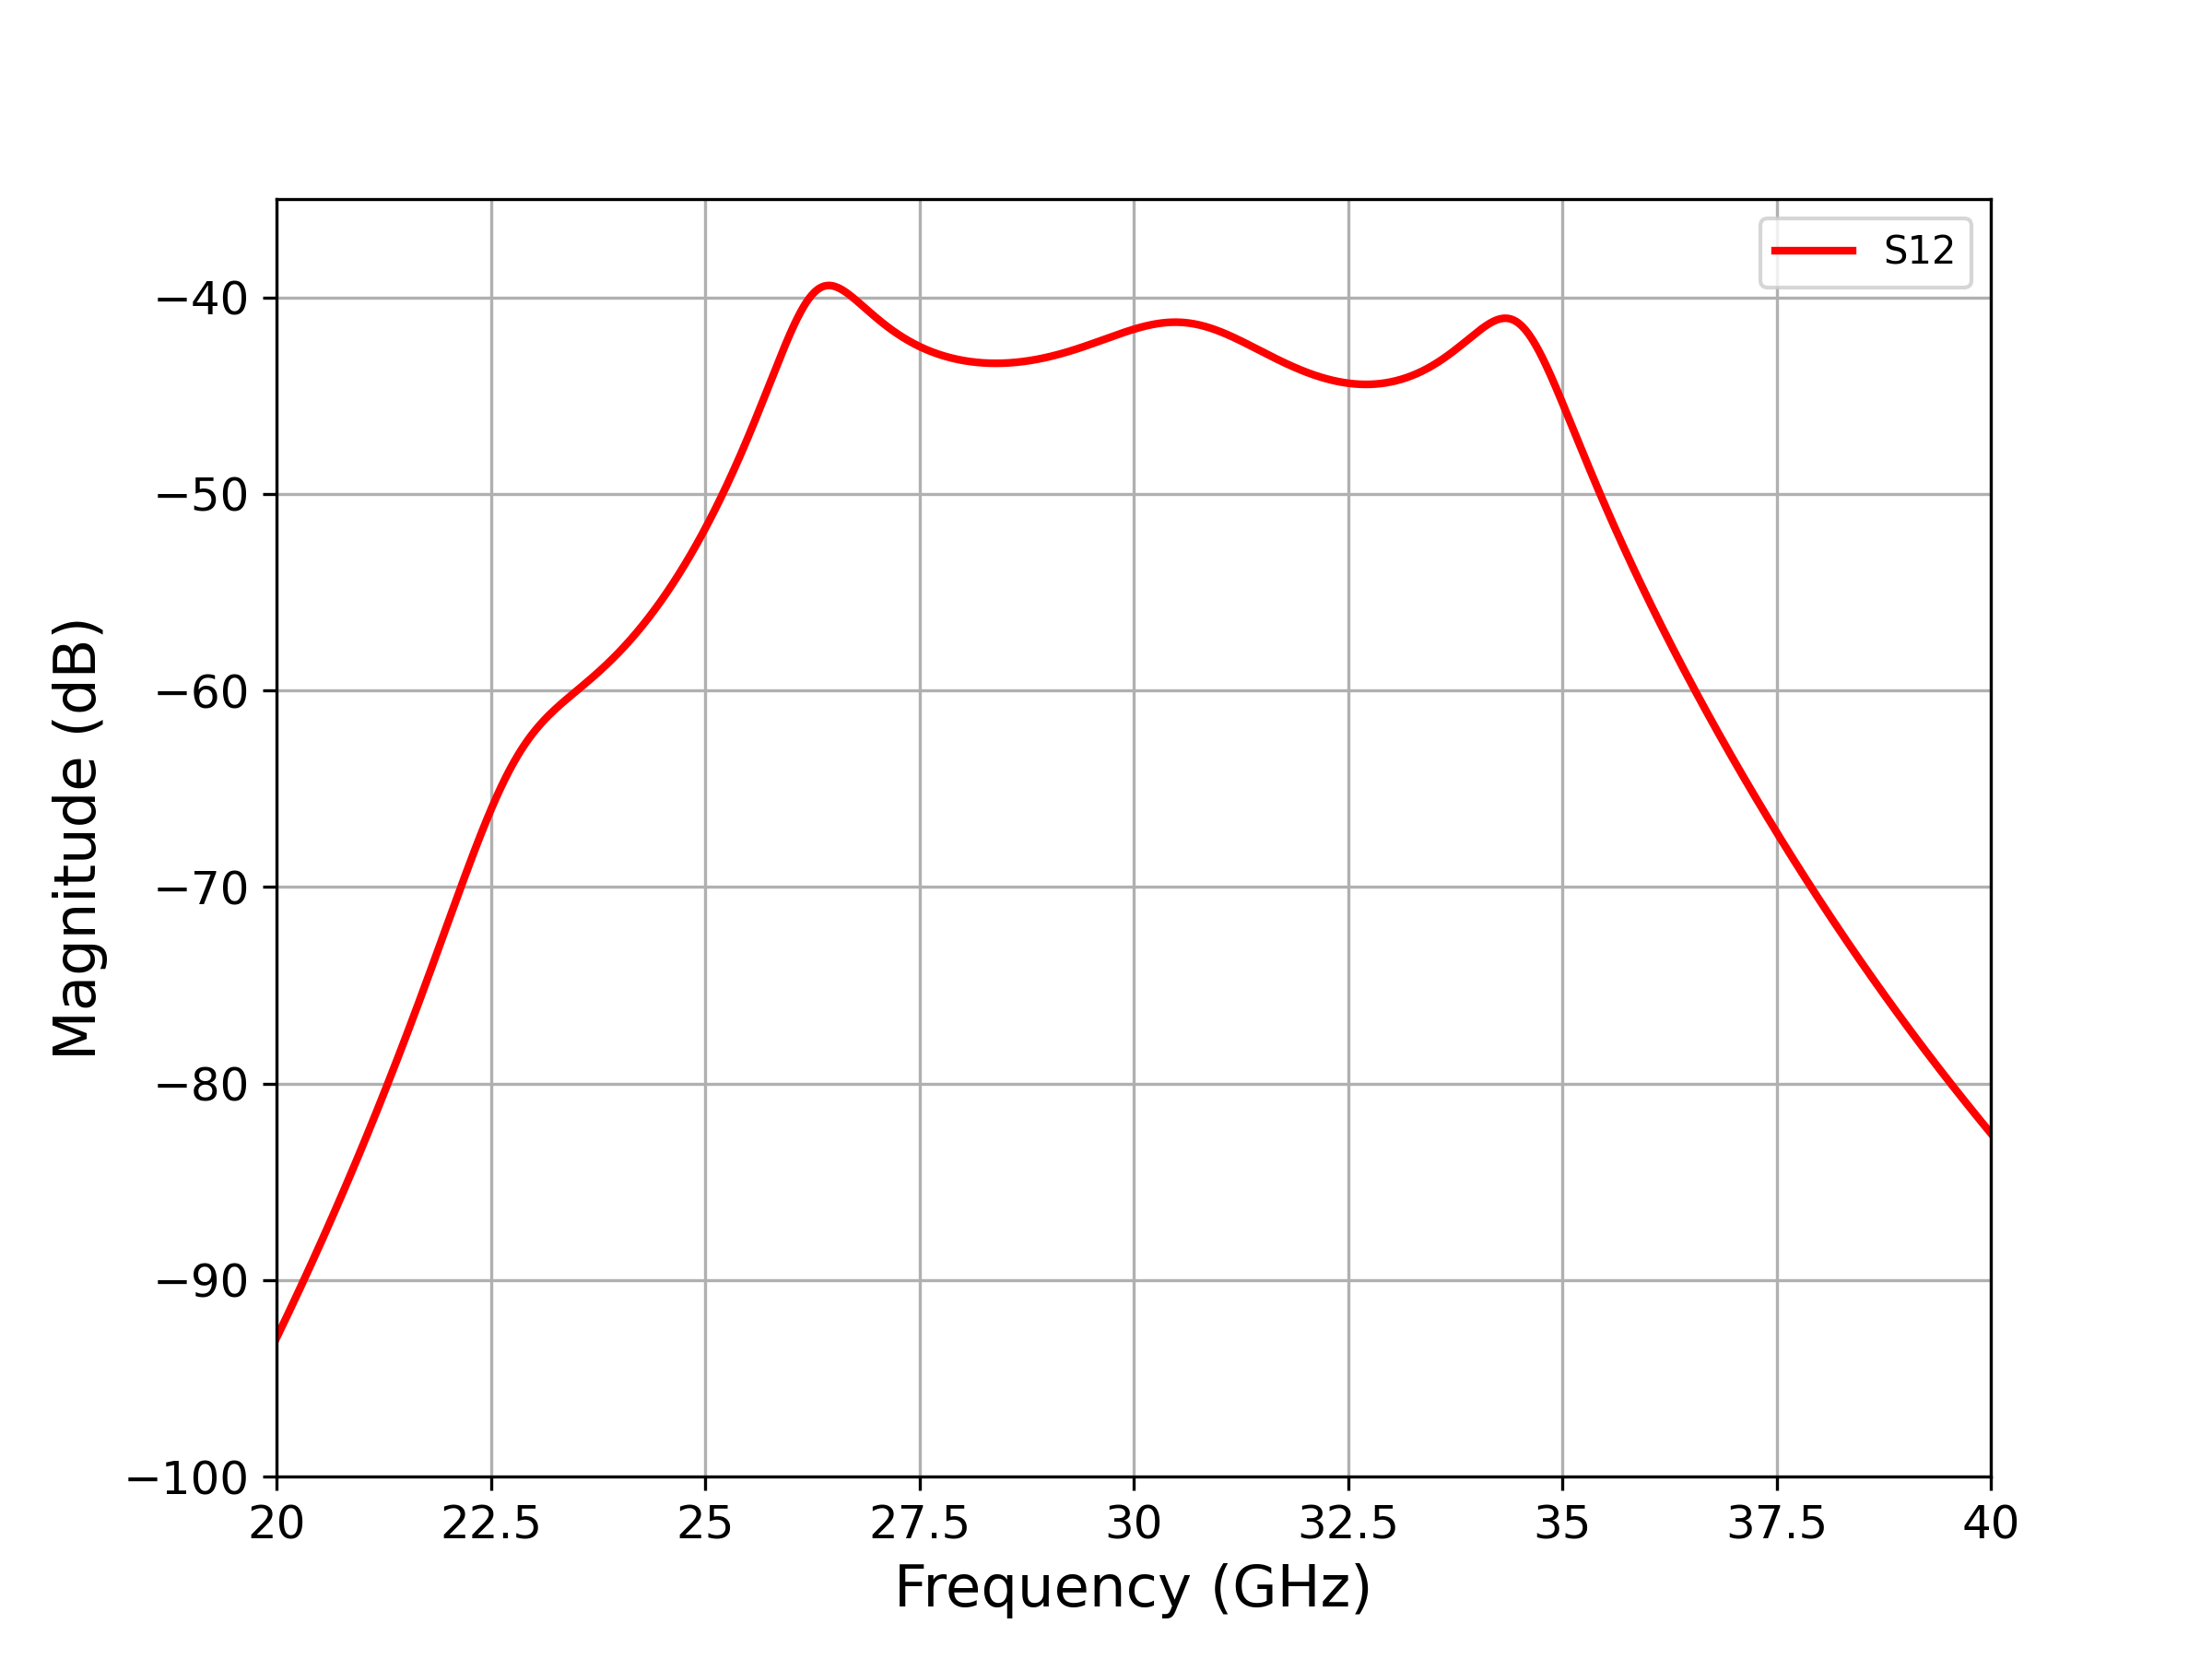
\includegraphics[]{figures/two_stage_withMatching_s12.png}
%     }
%     \caption{$S_{12}$ parameter of a two-stage power amplifier (shown in Figure \ref{fig:two-stage-with-input-interstage-matching}) with input and interstage matching network. The $S_{12}$ parameter is plotted from 0 GHz to 60 GHz.}
%     \label{fig:two-stage-withmatching-cadence-s12}
% \end{figure}

\begin{figure}[H]
  \centering
  \begin{subfigure}{0.49\textwidth}
    \centering
    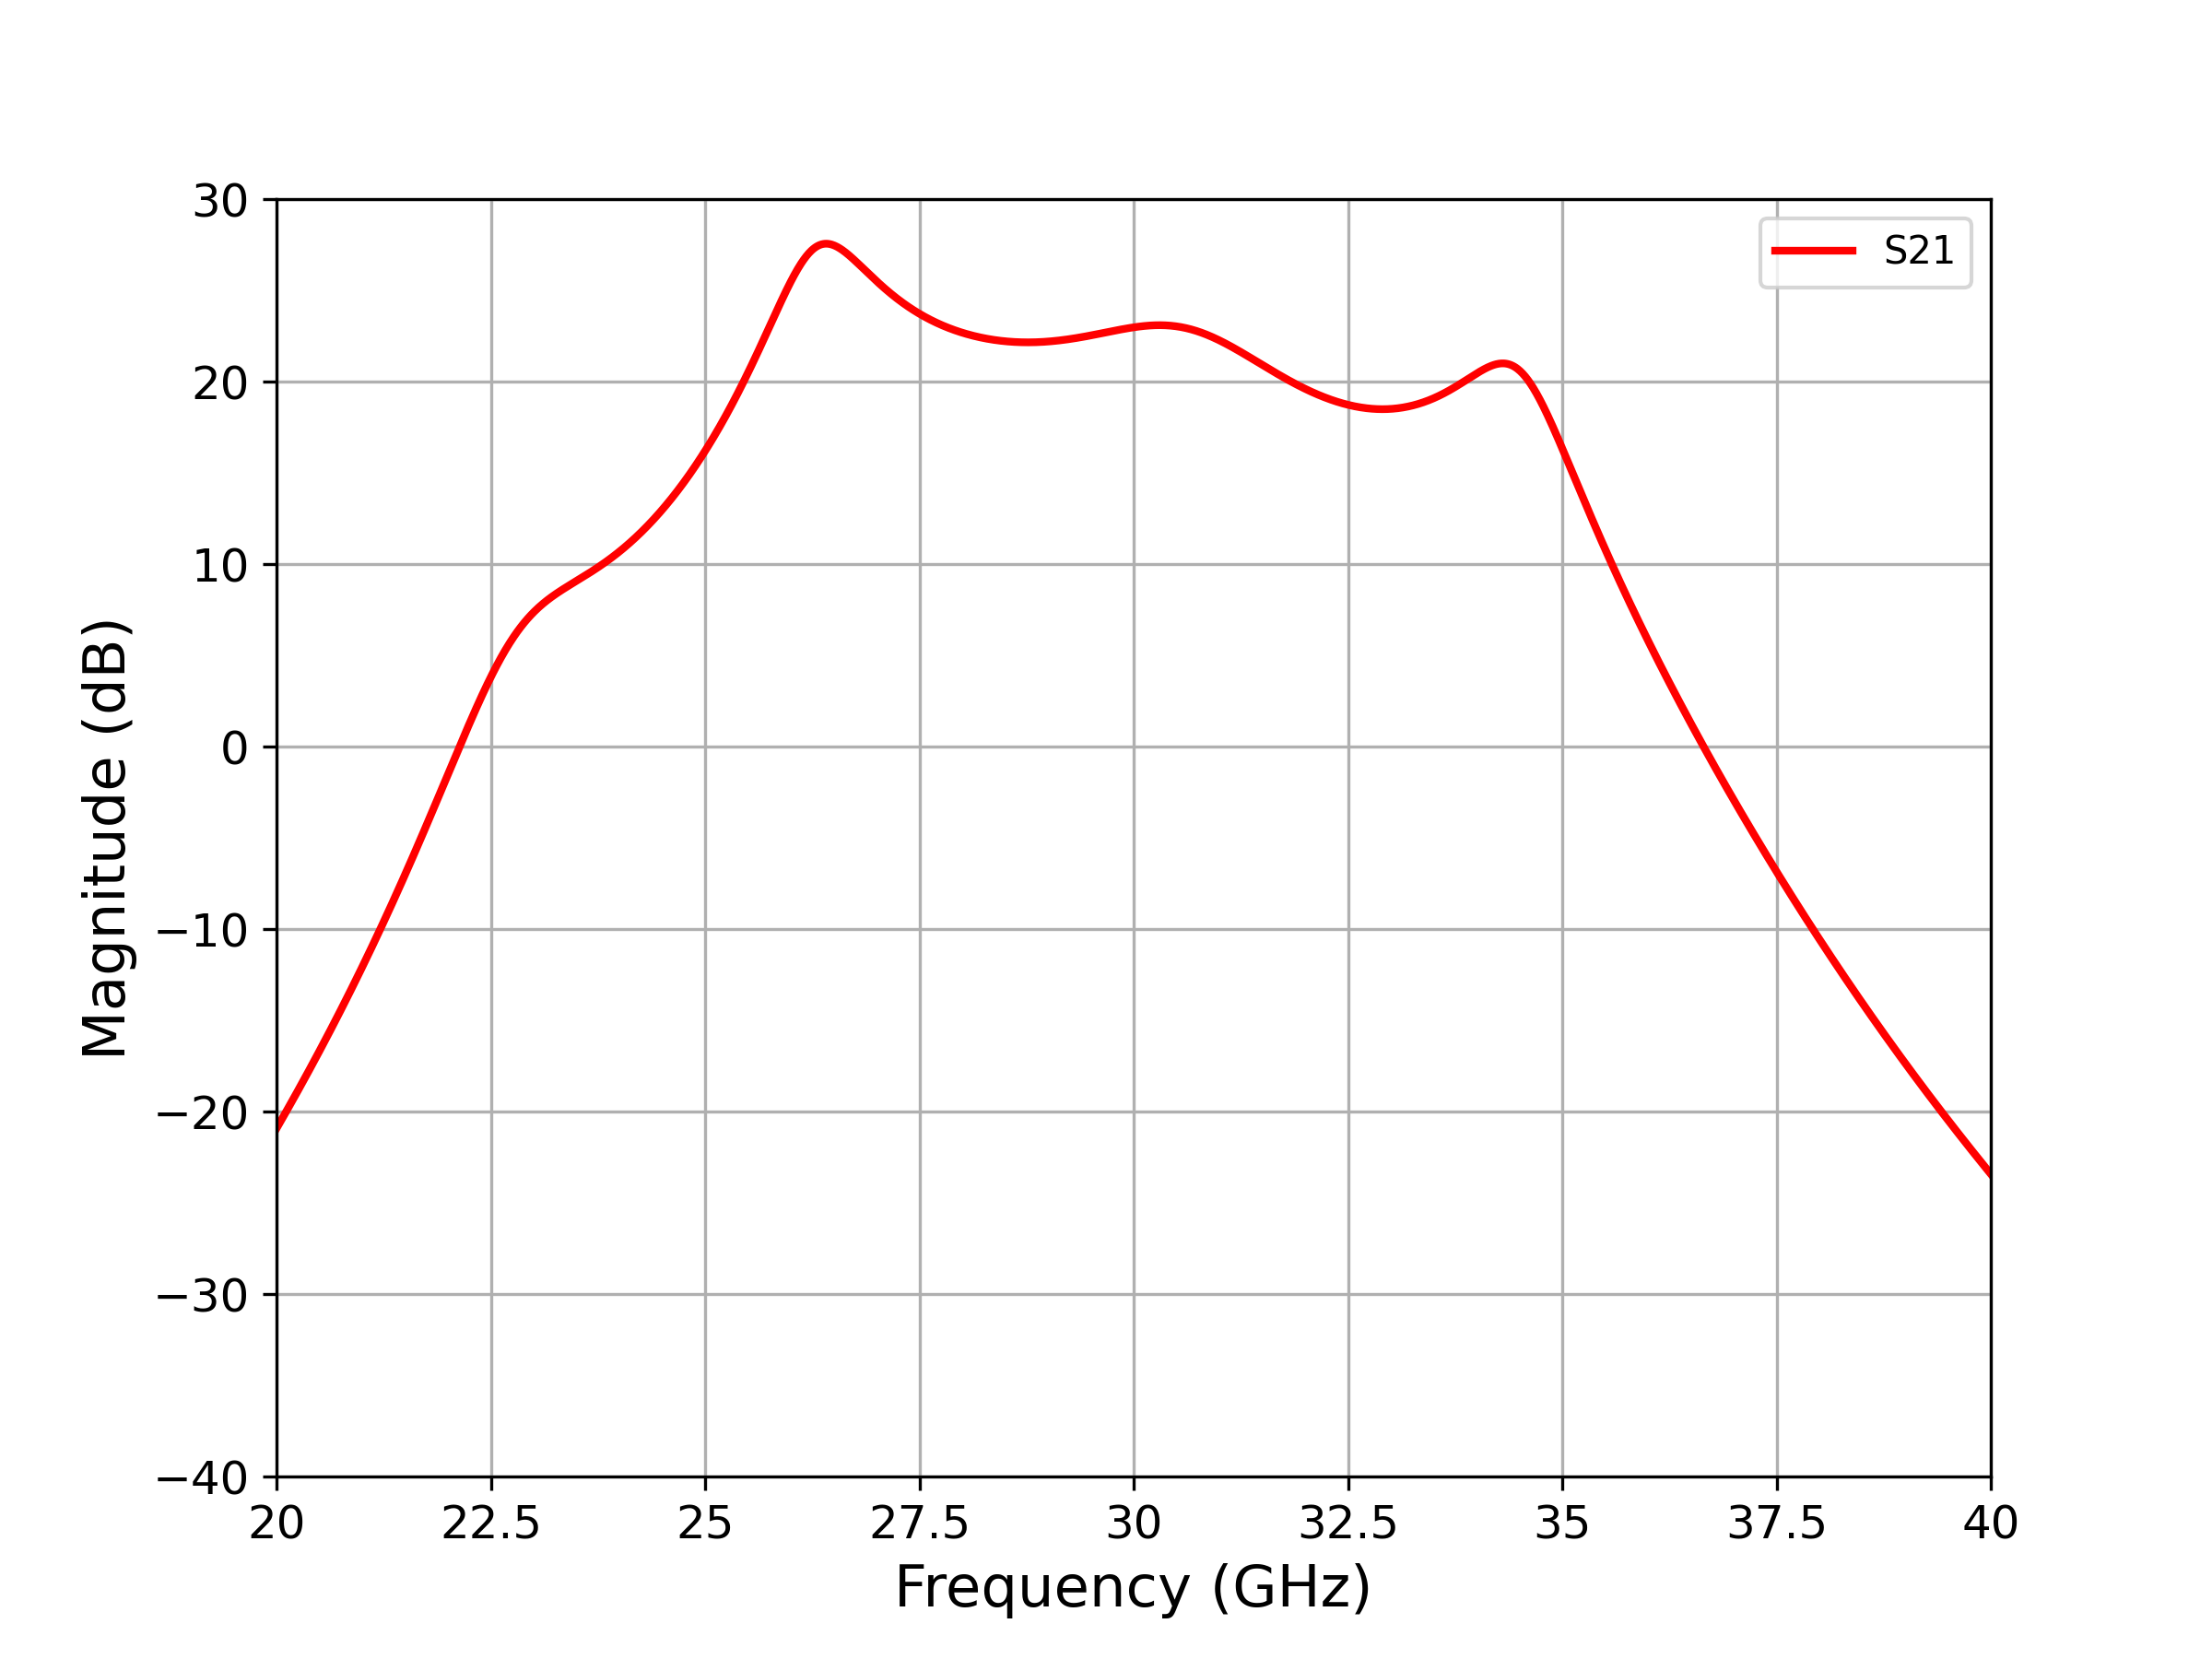
\includegraphics[width=\linewidth]{figures/two_stage_withMatching_s21.png}
    \caption{}
    \label{fig:two-stage-withmatching-cadence-s21}
  \end{subfigure}
  \hfill
  \begin{subfigure}{0.49\textwidth}
    \centering
    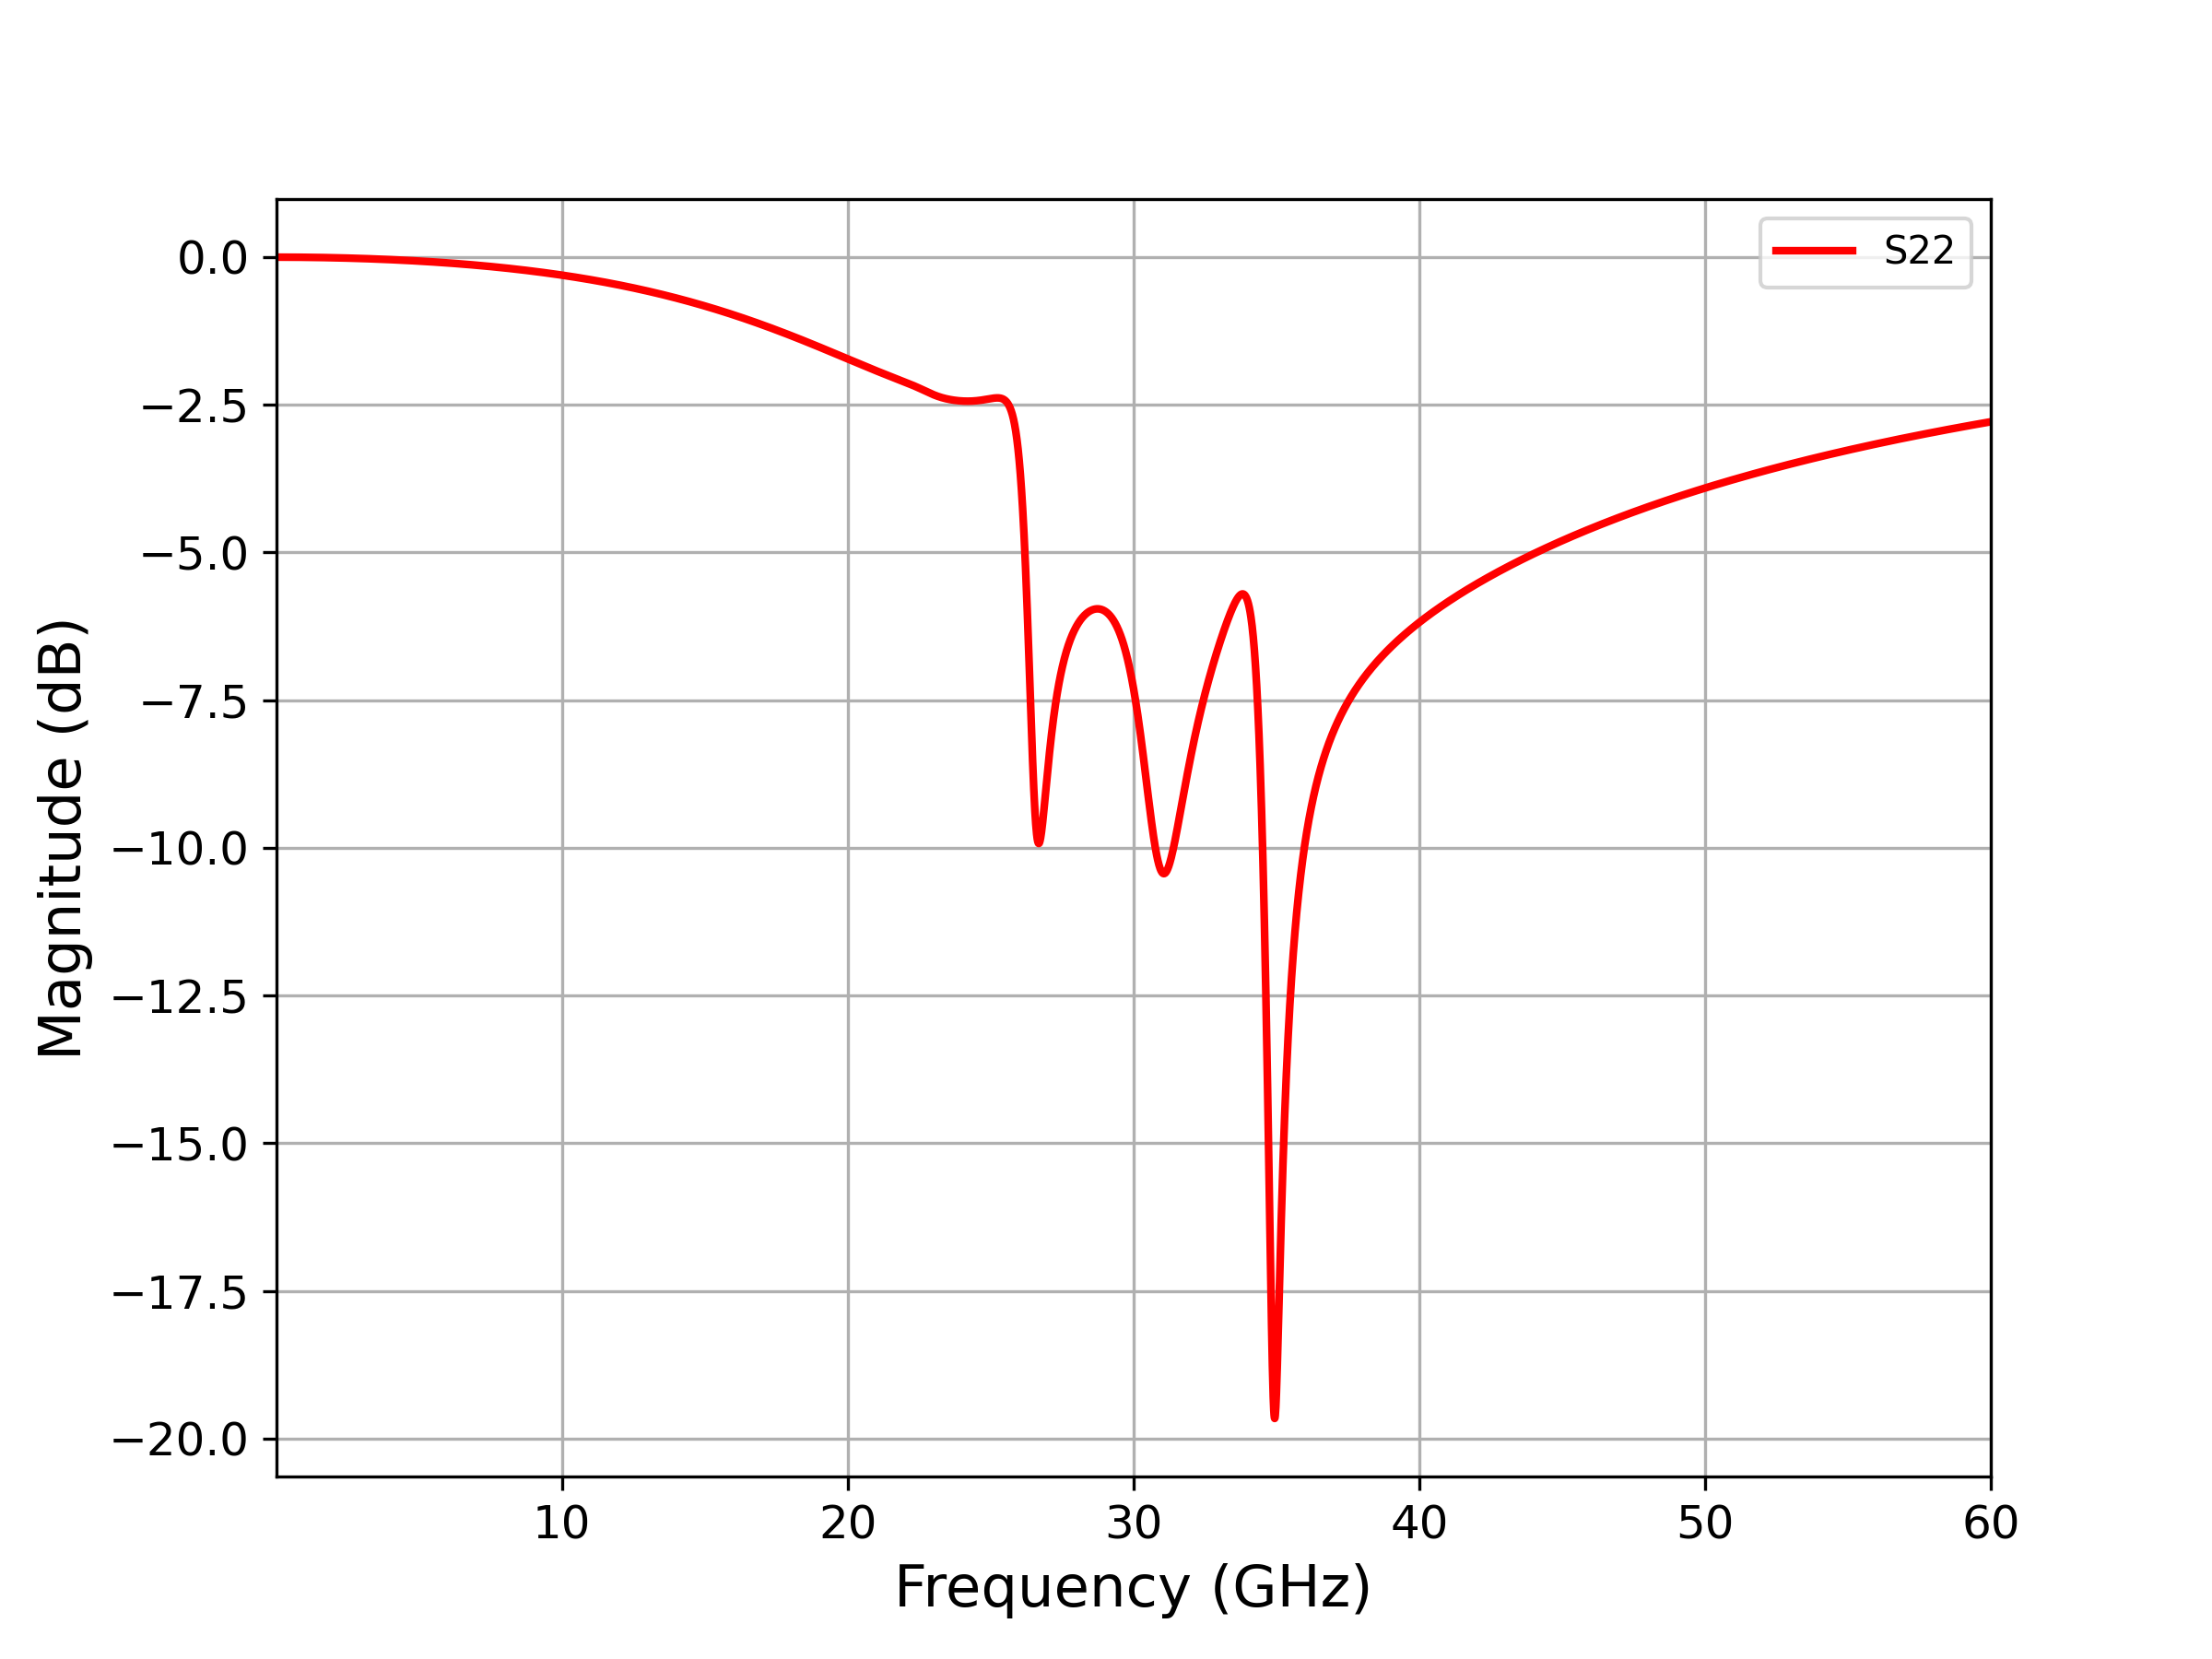
\includegraphics[width=\linewidth]{figures/two_stage_withMatching_s22.png}
    \caption{}
     \label{fig:two-stage-withmatching-cadence-s22}
  \end{subfigure}
  \caption{(a) $S_{21}$ parameter of a two-stage power amplifier (shown in Figure \ref{fig:two-stage-with-input-interstage-matching}) with input and interstage matching network. (b) $S_{22}$ parameter of a two-stage power amplifier (shown in Figure \ref{fig:two-stage-with-input-interstage-matching}) with input and interstage matching network.}
  \label{fig:two-stage-withmatching-cadence-s21-s22}
\end{figure}

The maximum value of $S_{21}$ at 26.41 GHz is 27.55 dB, indicating a
higher power gain compared to the previous stages. Average gain and
gain at matching frequencies: The average gain across the frequency range
of 25 to 35 GHz is 21.78 dB. At the matching frequencies of 27.12 GHz and
32.33 GHz, the gain values are 25 dB and 18.96 dB, respectively. These
gains demonstrate the improvement achieved through the matching network. The proposed PA exhibits good output matching
with $S_{22}$ values of less than -5 dB, indicating that a small portion of the
output power is reflected back.
% \begin{figure}[H]
%     \centering
%     \resizebox{0.8\textwidth}{!}{
%     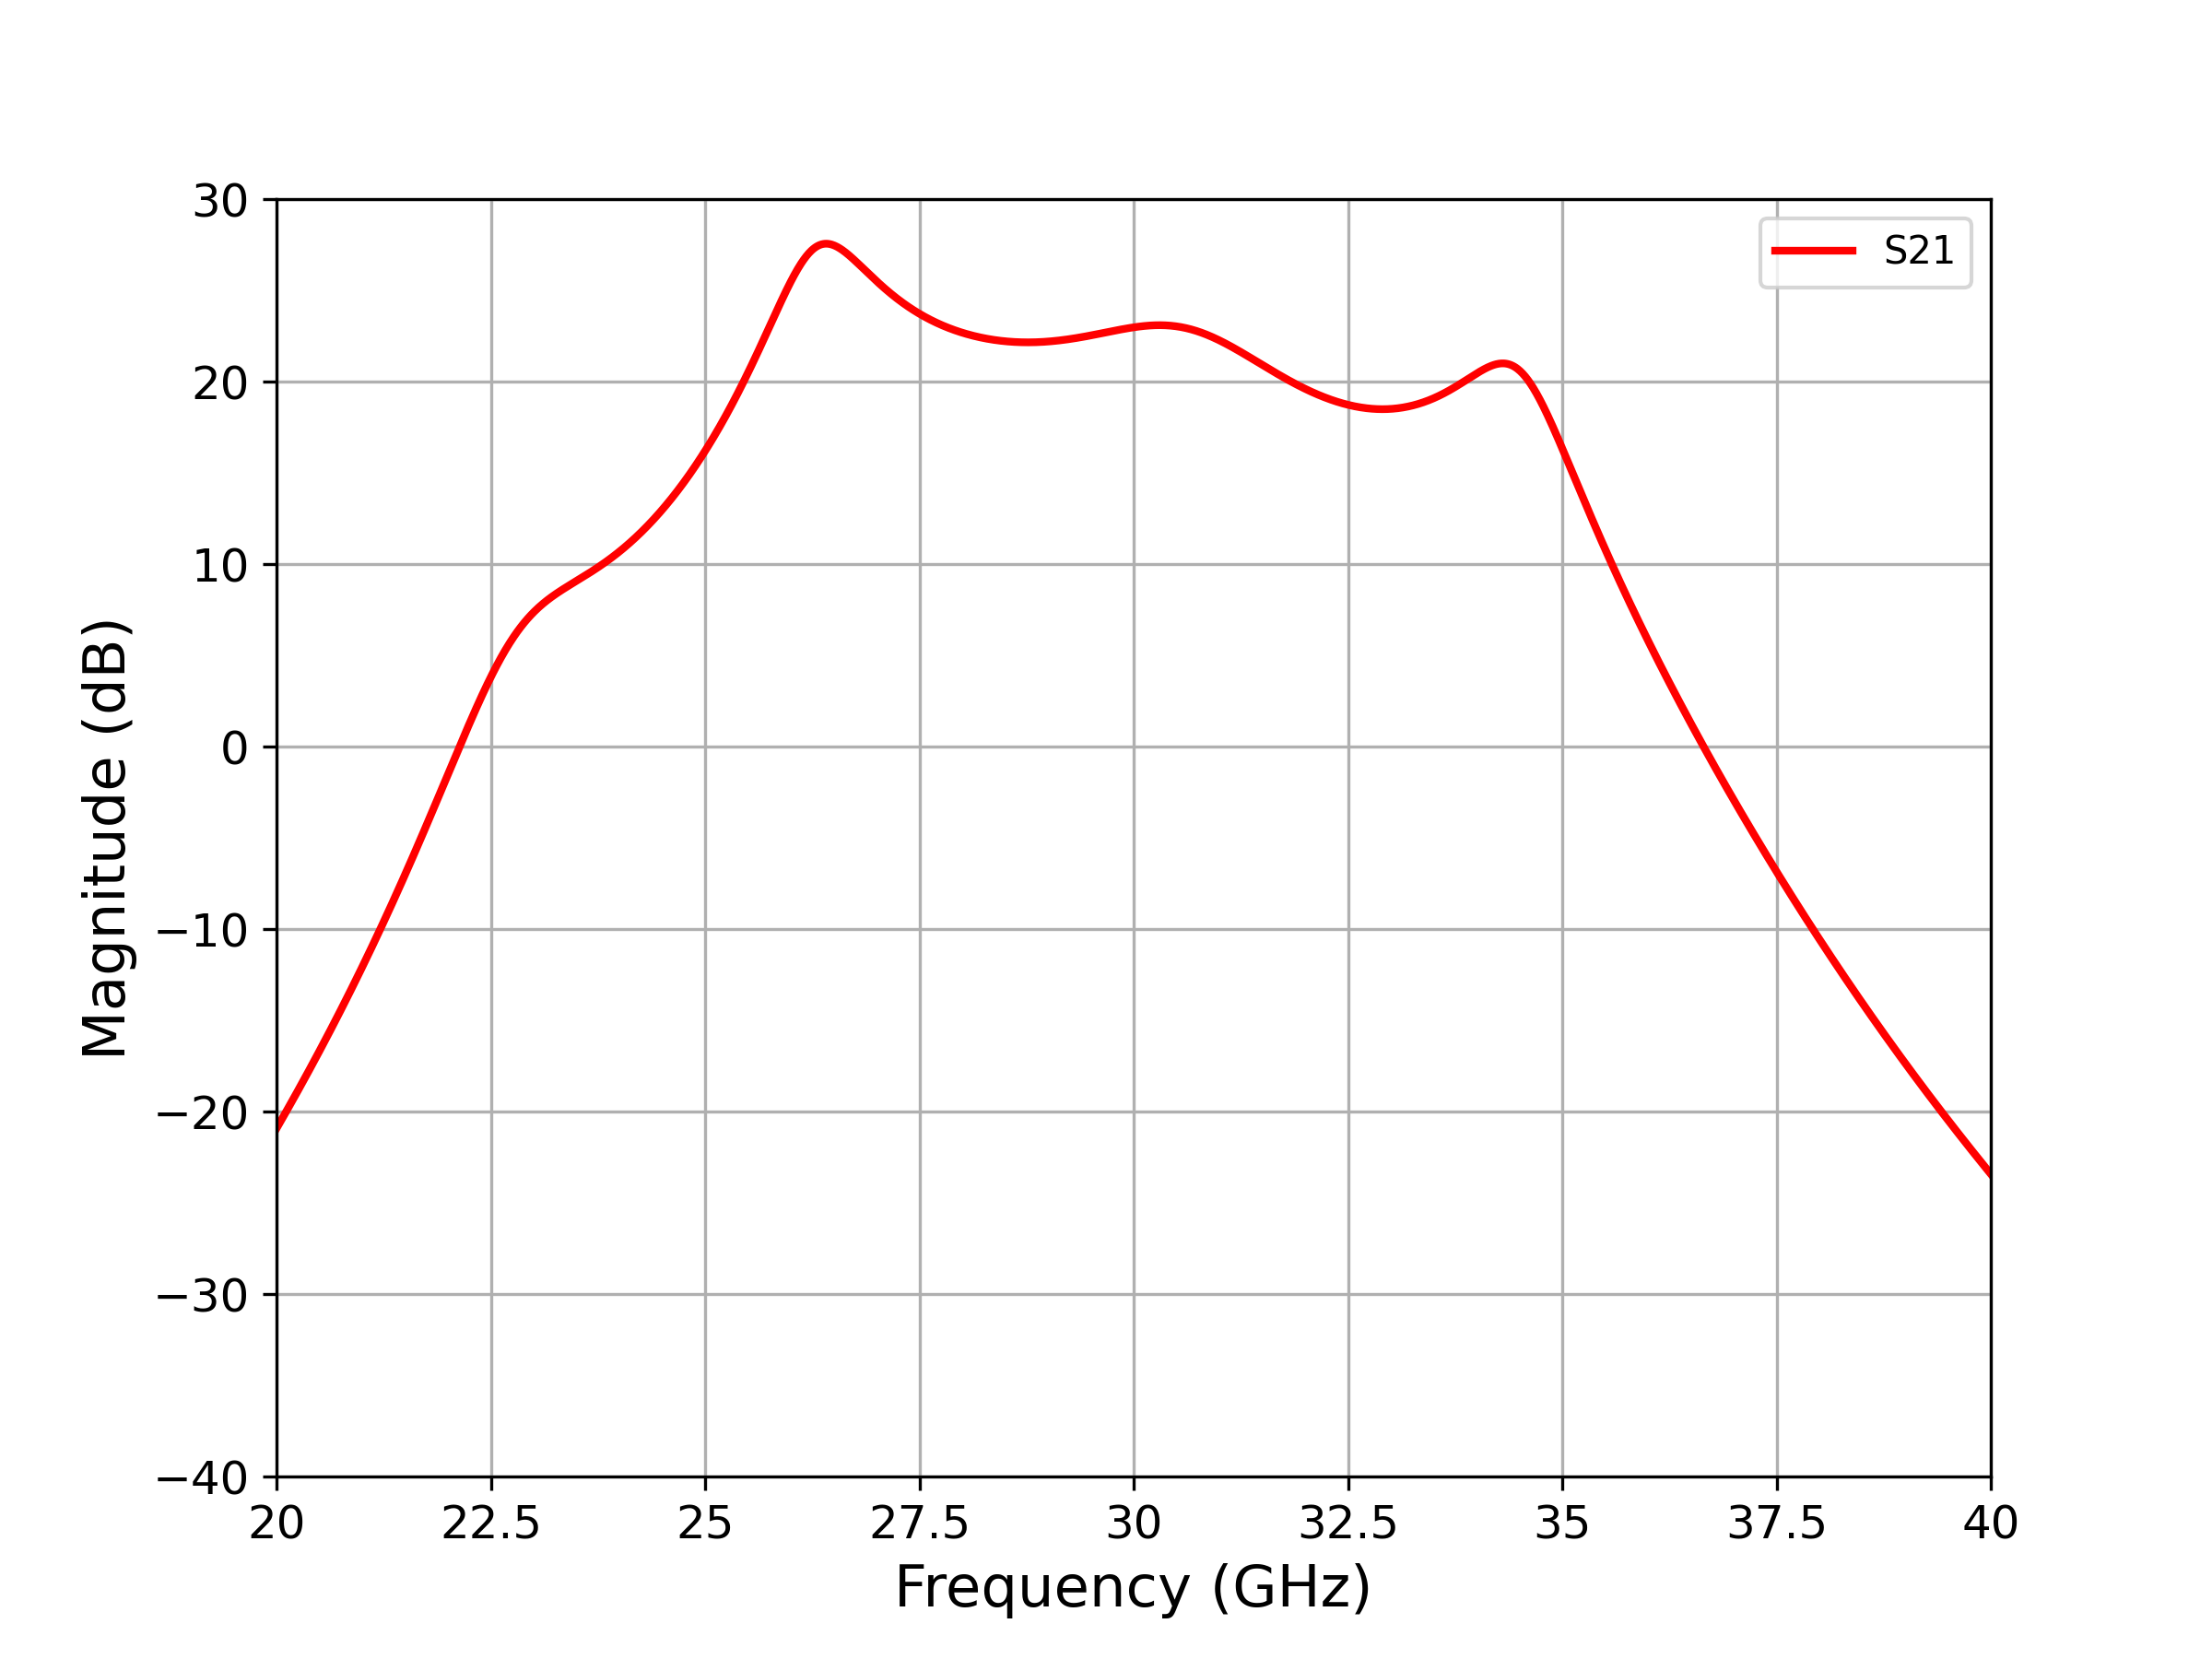
\includegraphics[]{figures/two_stage_withMatching_s21.png}
%     }
%     \caption{$S_{21}$ parameter of a two-stage power amplifier (shown in Figure \ref{fig:two-stage-with-input-interstage-matching}) with input and interstage matching network. The $S_{21}$ parameter is plotted from 20 GHz to 40 GHz.}
%     \label{fig:two-stage-withmatching-cadence-s21}
% \end{figure}
% \begin{figure}[H]
%     \centering
%     \resizebox{0.8\textwidth}{!}{
%     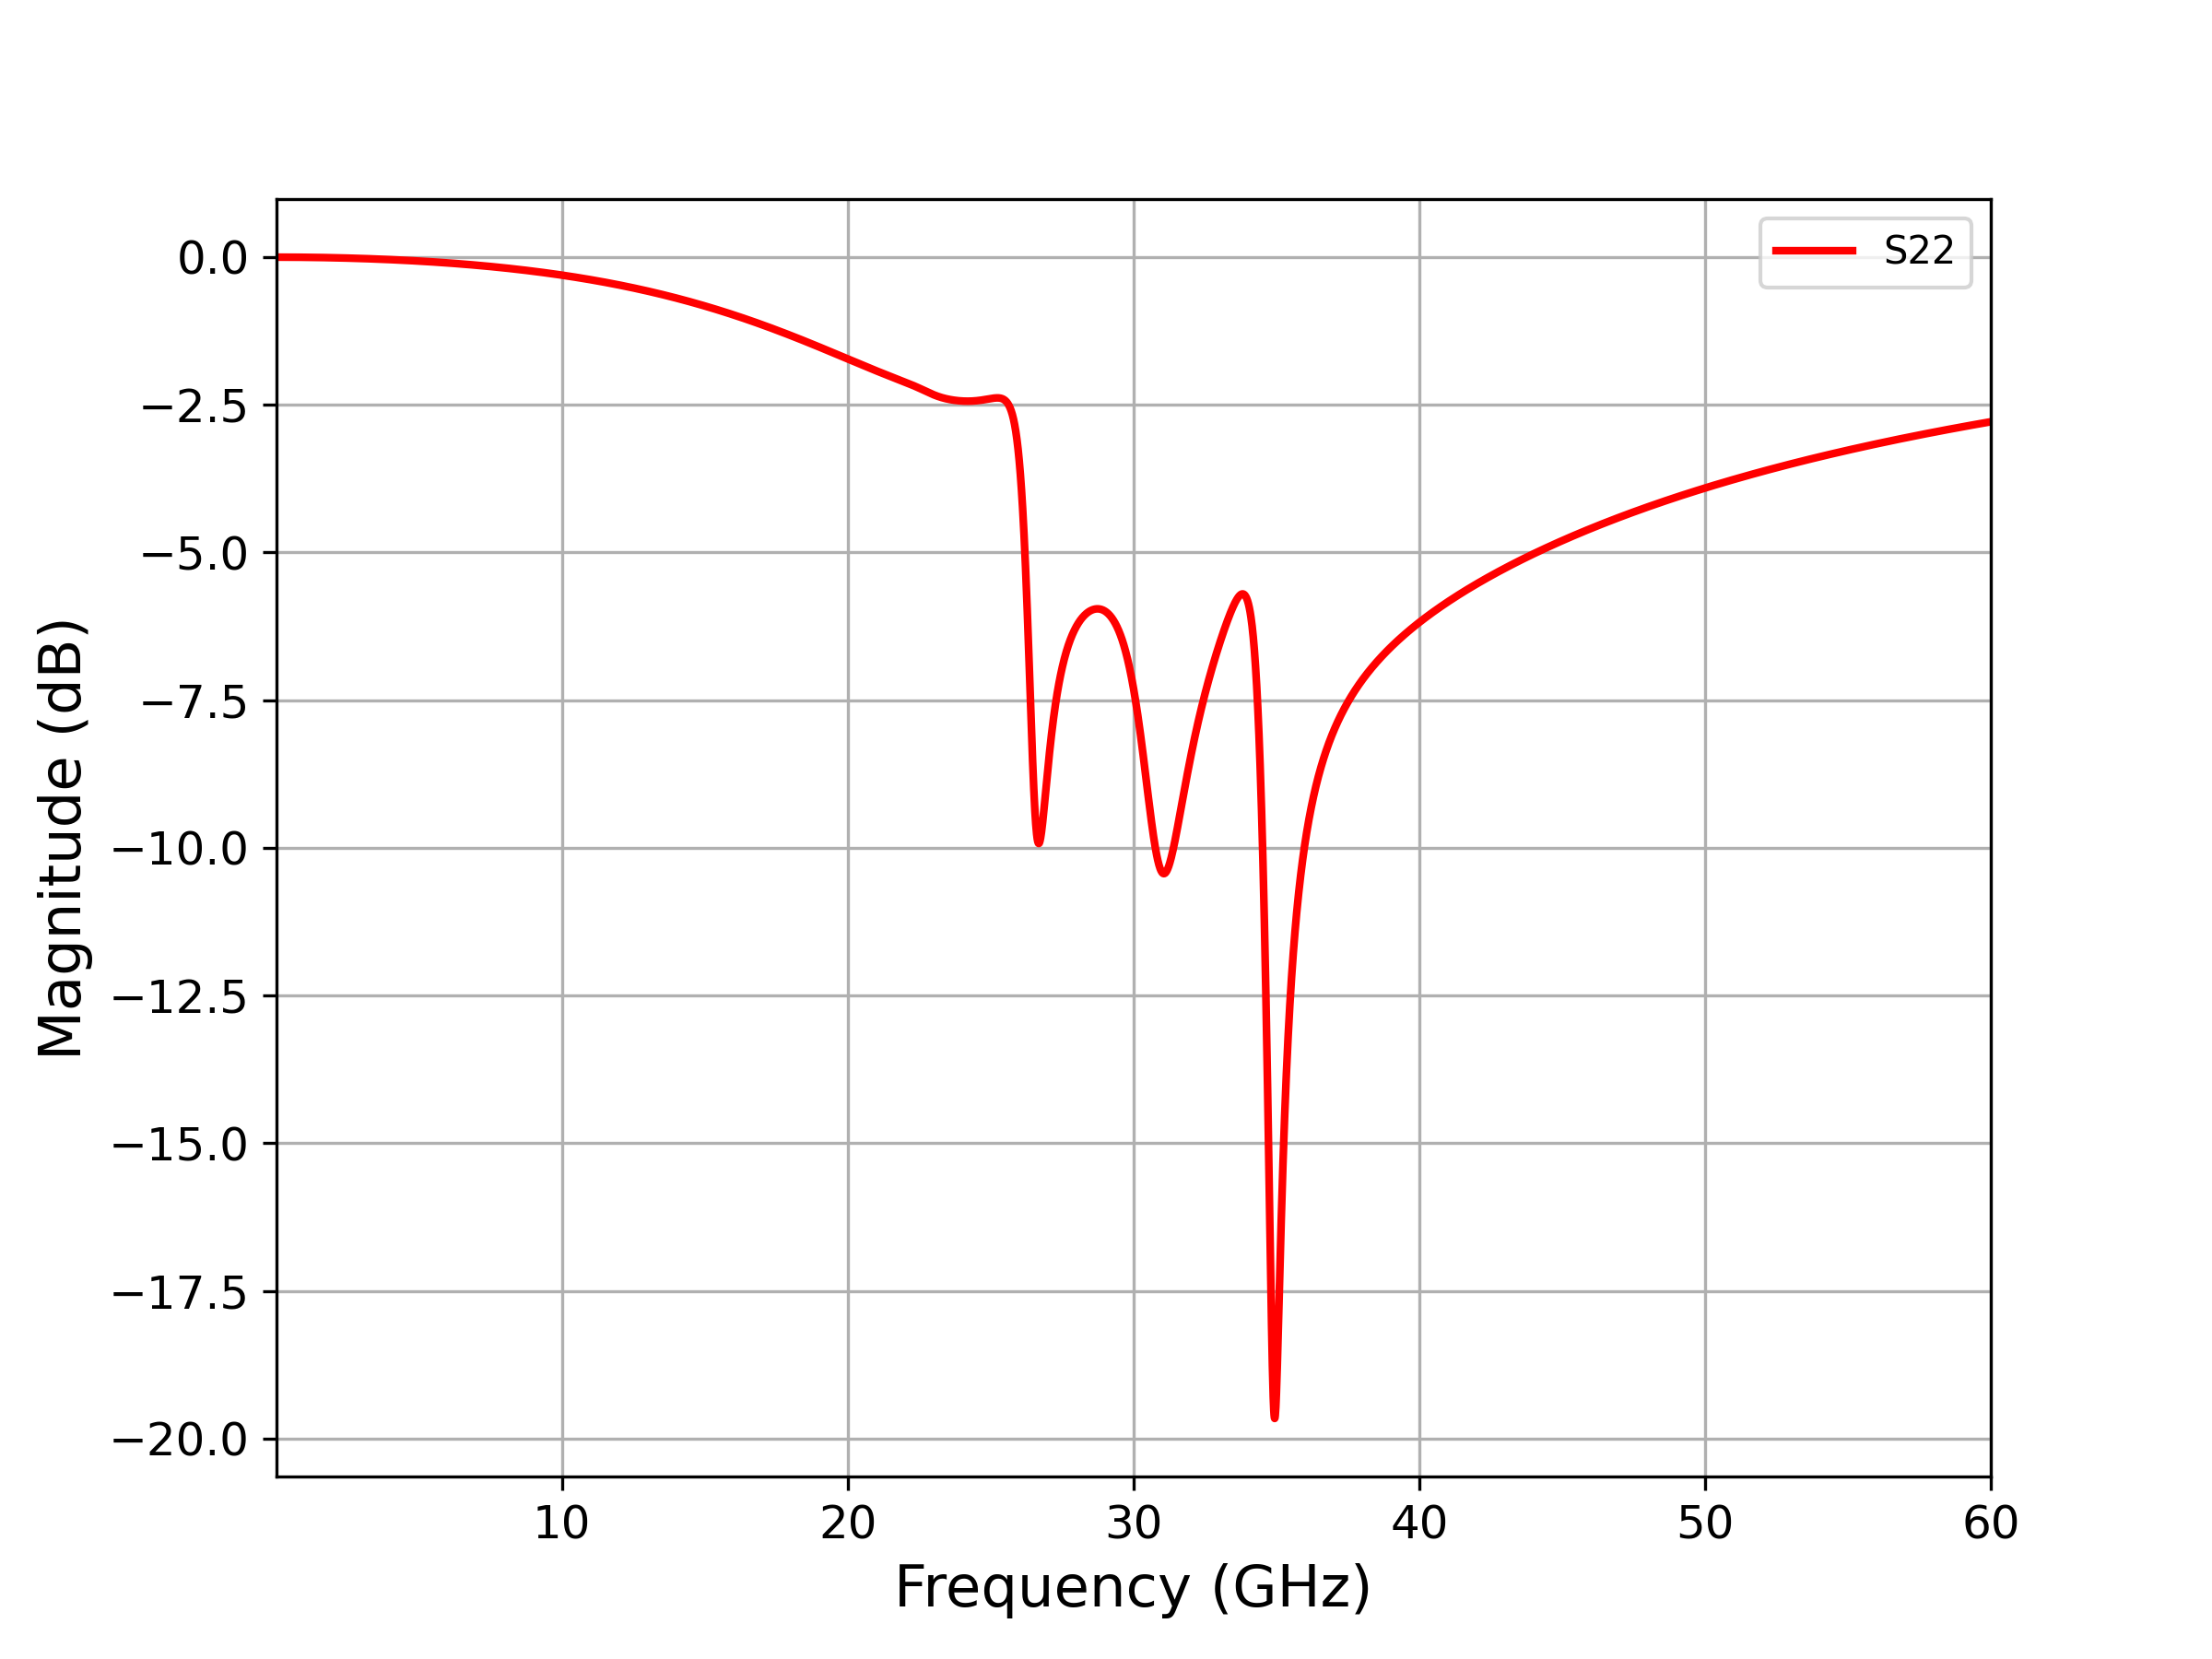
\includegraphics[]{figures/two_stage_withMatching_s22.png}
%     }
%     \caption{$S_{22}$ parameter of a two-stage power amplifier (shown in Figure \ref{fig:two-stage-with-input-interstage-matching}) with input and interstage matching network. The $S_{22}$ parameter is plotted from 0 GHz to 60 GHz.}
%     \label{fig:two-stage-withmatching-cadence-s22}
% \end{figure}
\begin{figure}[H]
  \centering
  \begin{subfigure}{0.49\textwidth}
    \centering
    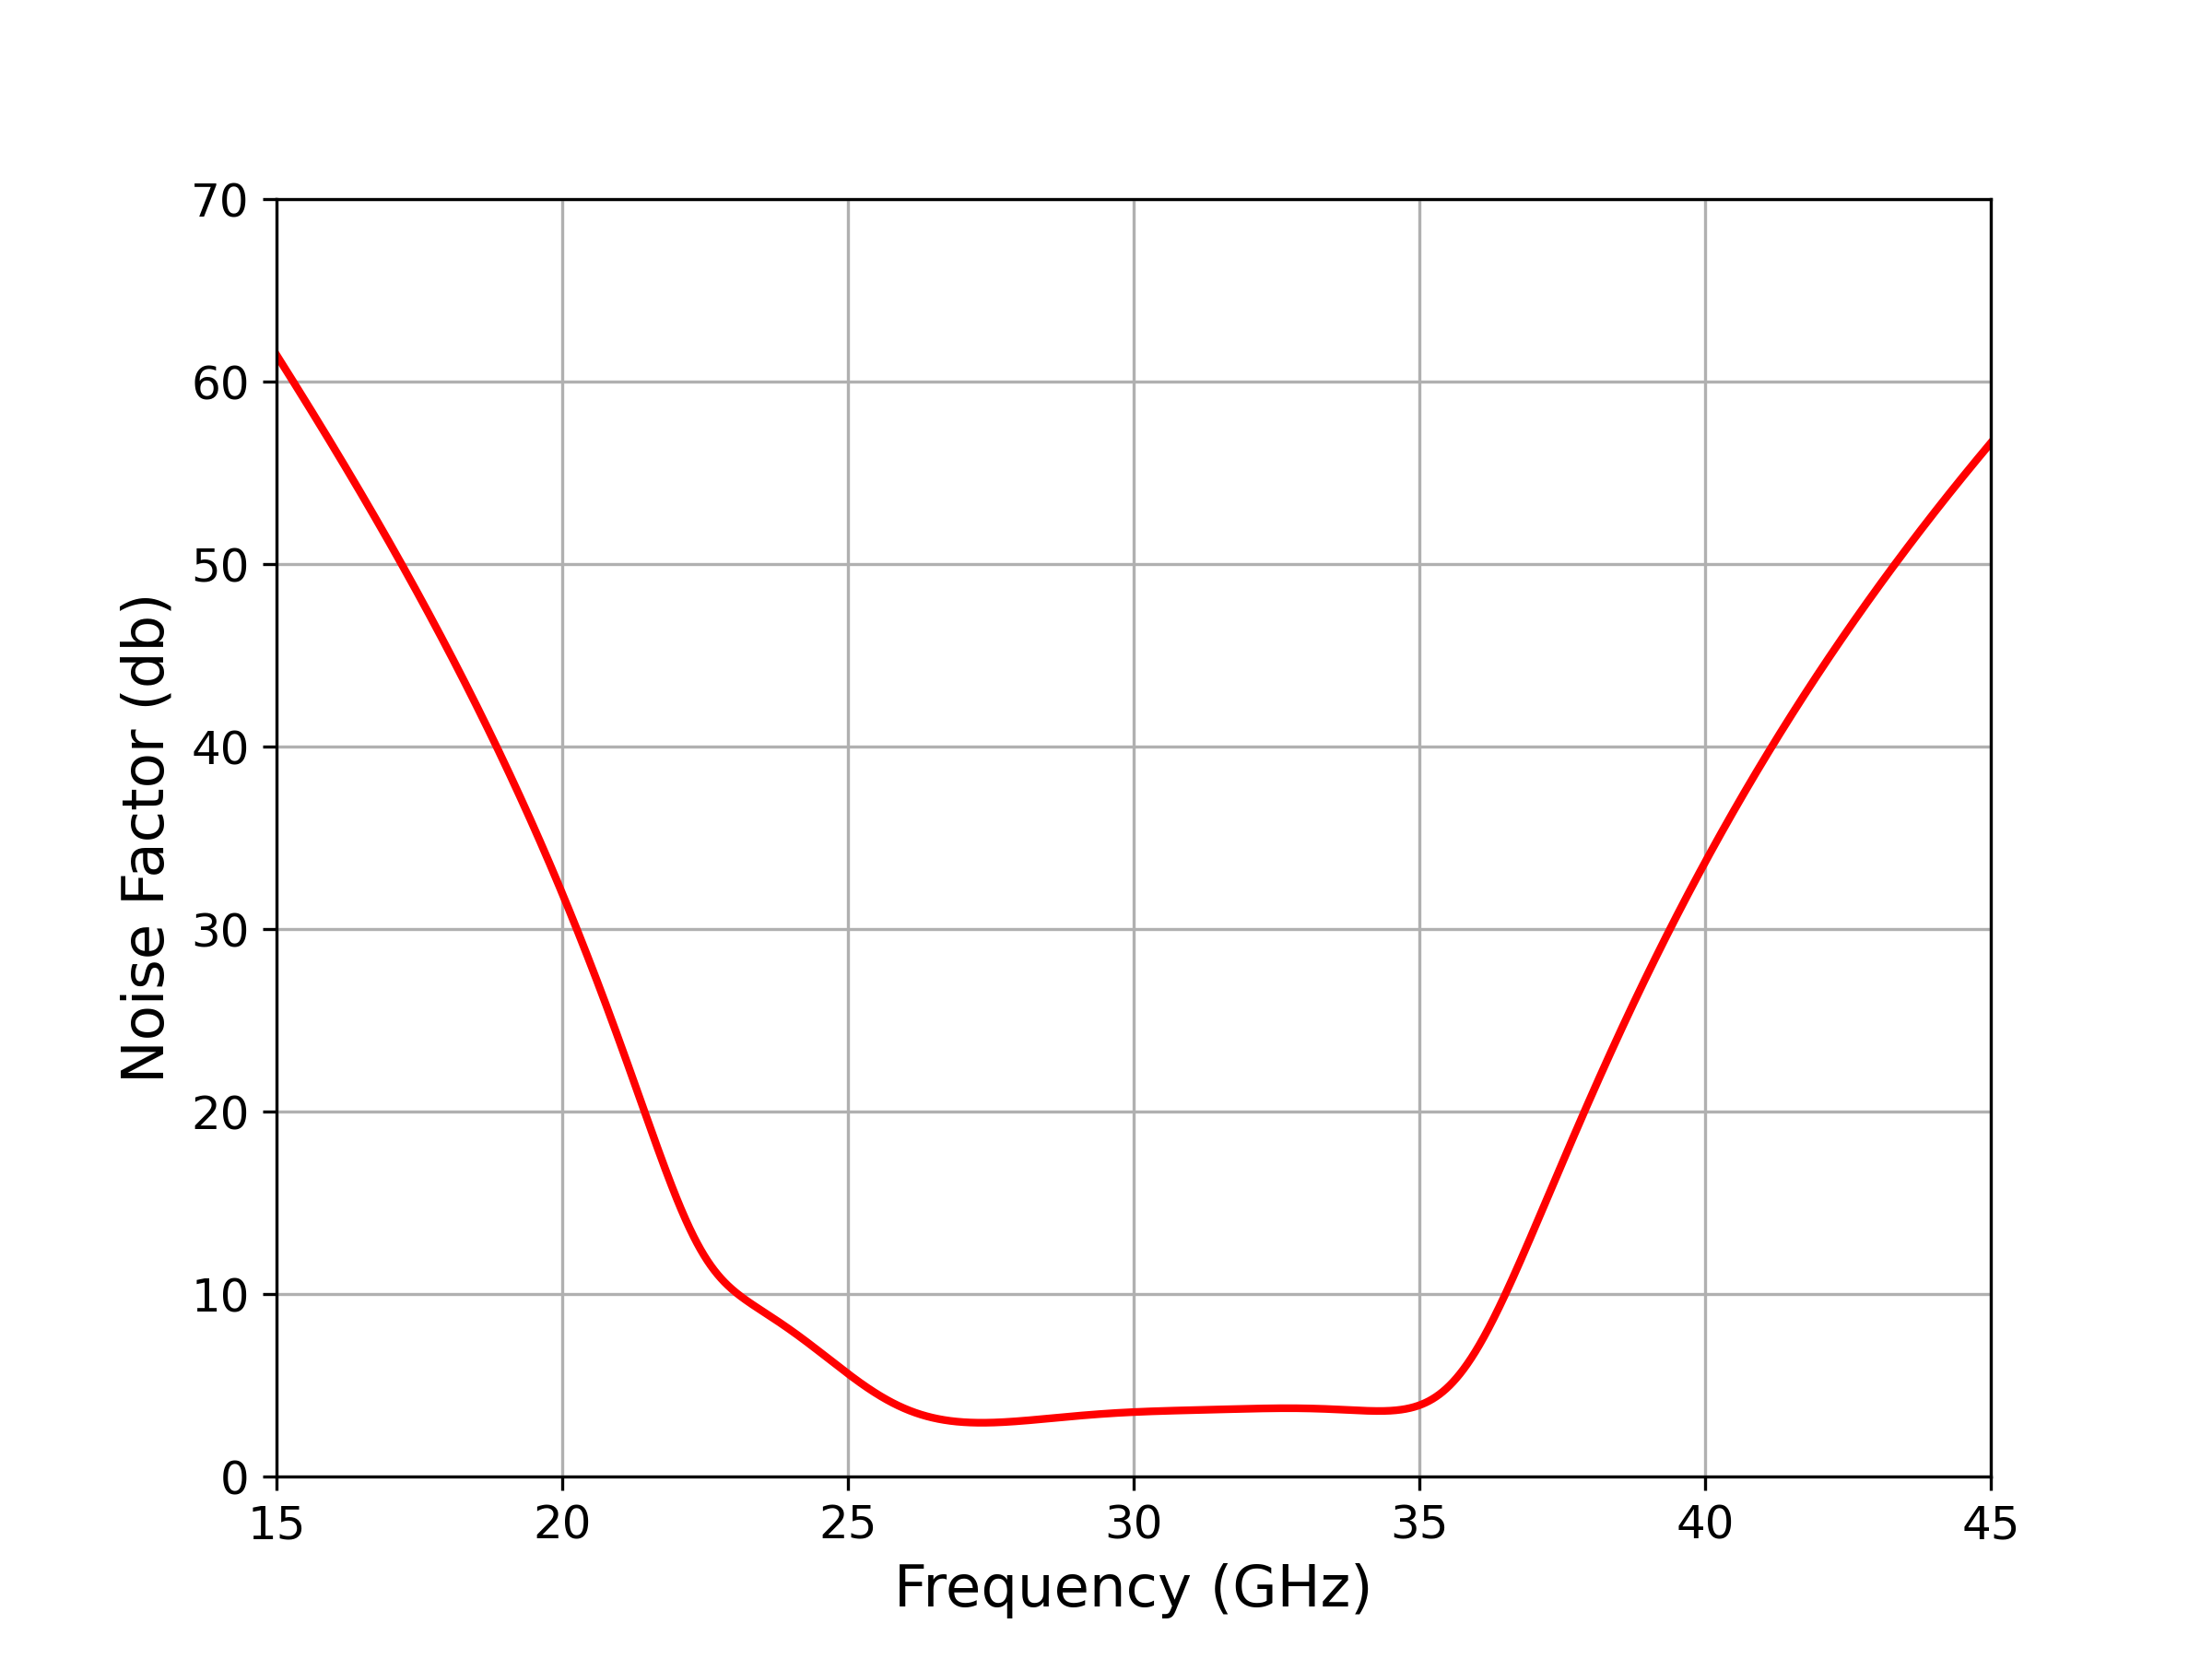
\includegraphics[width=\linewidth]{figures/noise-factor.png}
    \caption{}
    \label{fig:noise-factor}
  \end{subfigure}
  \hfill
  \begin{subfigure}{0.49\textwidth}
    \centering
    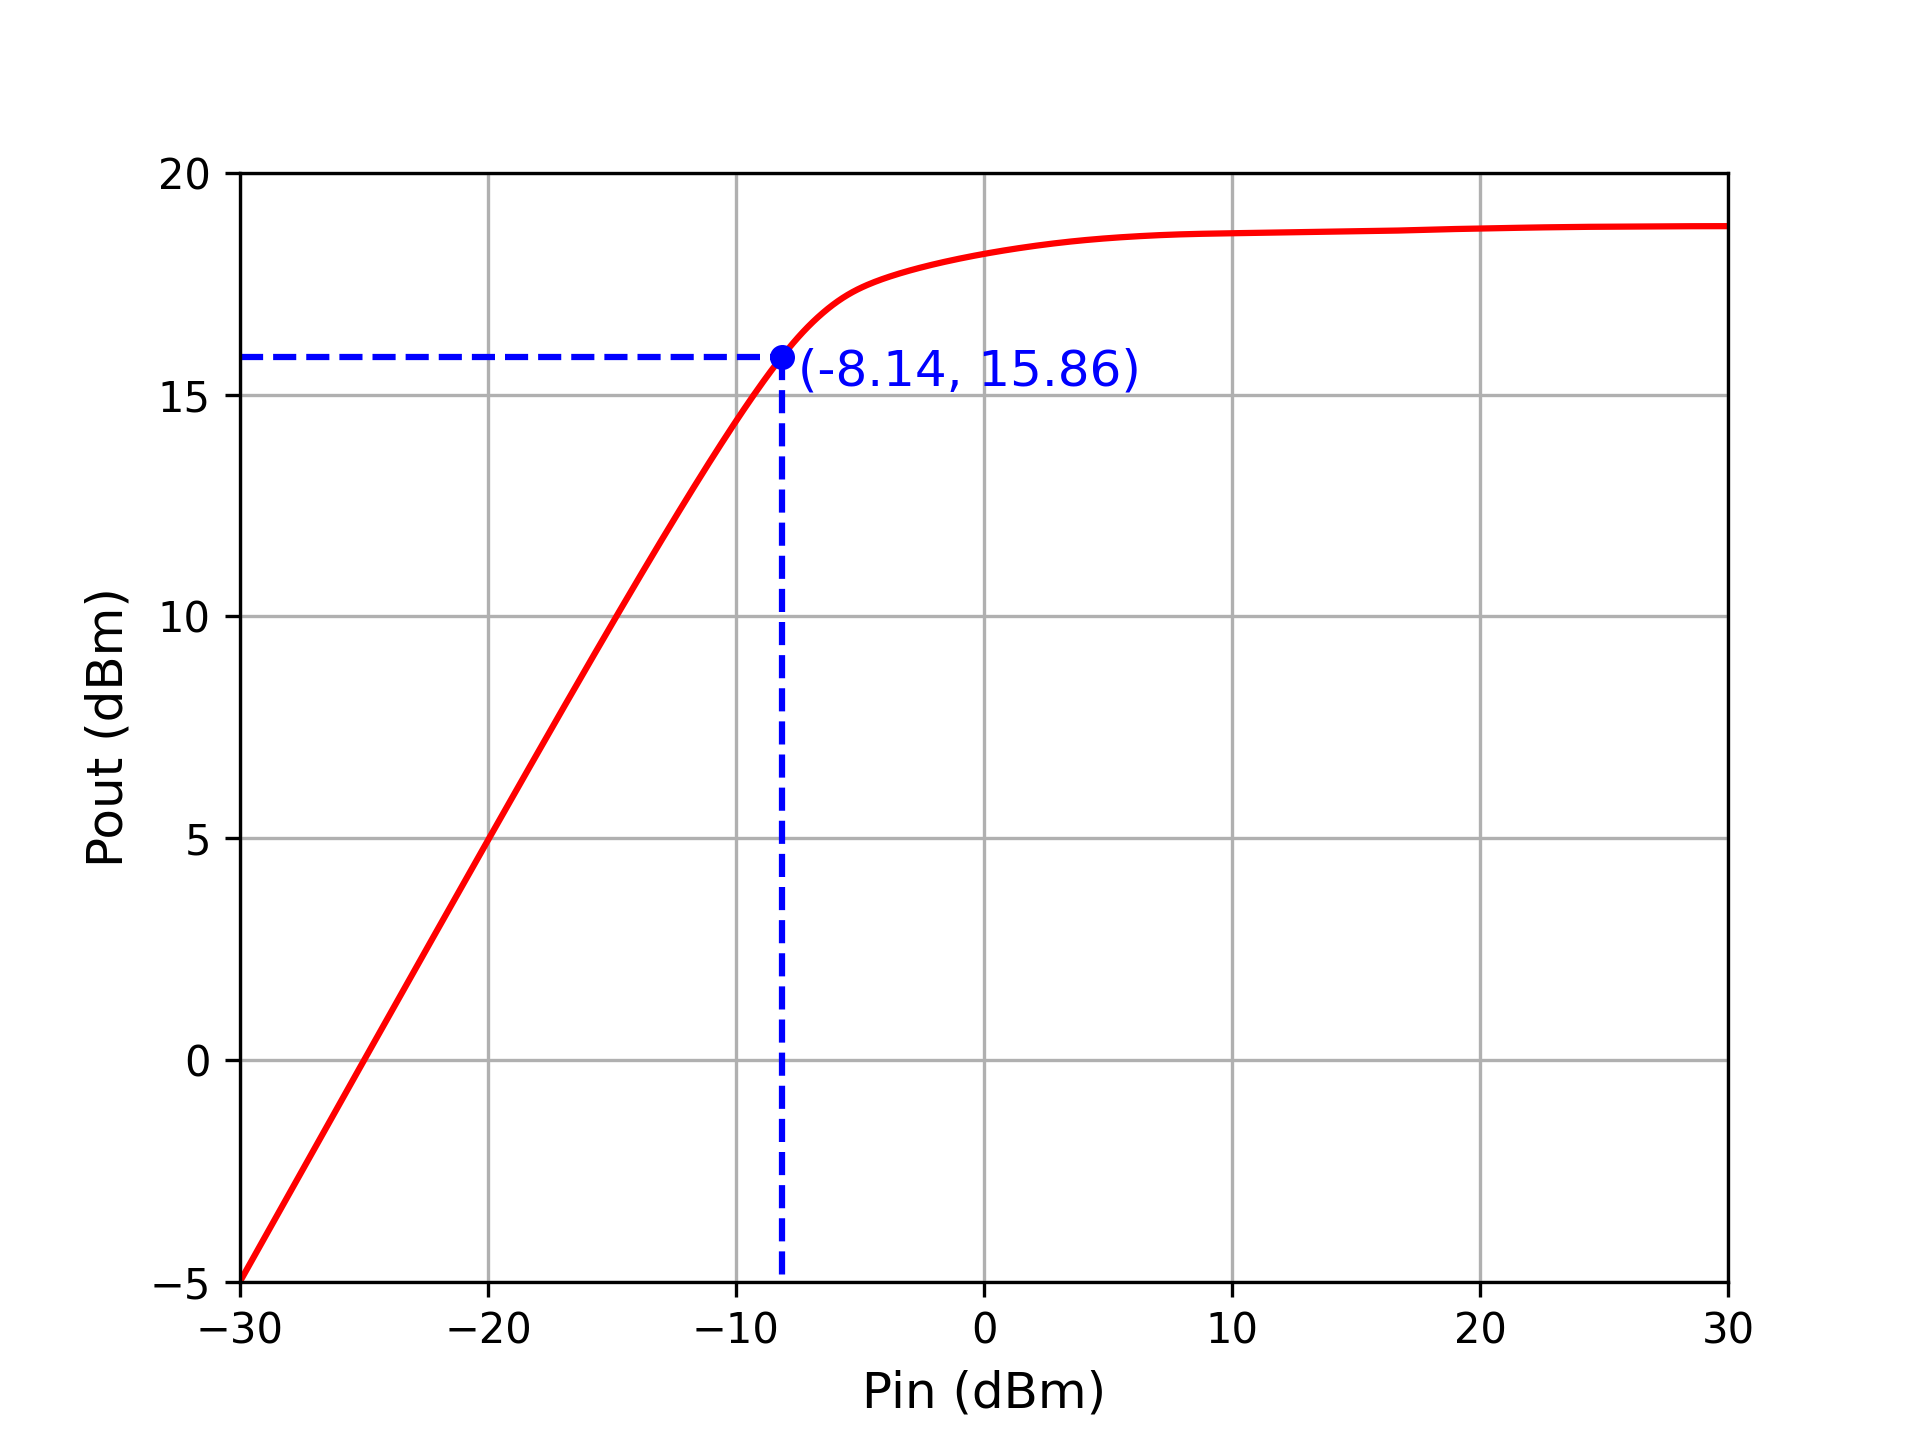
\includegraphics[width=\linewidth]{figures/compressionCurves.png}
    \caption{}
     \label{fig:compression}
  \end{subfigure}
  \caption{(a) Noise factor of a two-stage power amplifier (shown in Figure \ref{fig:two-stage-with-input-interstage-matching}) with input and interstage matching network. (b) P1db compression curve of a two-stage power amplifier (shown in Figure \ref{fig:two-stage-with-input-interstage-matching}) with input and interstage matching network.}
  \label{fig:two-stage-withmatching-cadence-s11-s12}
\end{figure}

The noise factor of a power amplifier is a measure of how much the amplifier degrades the signal-to-noise ratio of the input signal. A lower noise factor indicates better performance, as it means that the amplifier is introducing less additional noise to the signal. Ideally, a power amplifier should have a noise factor as close to 1 as possible, indicating that it adds minimal noise to the input signal. The noise factor of proposed PA is less than 5 dB through 25 GHz to 35 GHz. The P1dB of the proposed PA is (-8.14 dBm,
15.86 dBm). This refers to the output power level at which the gain decreases by
1 dB from its constant value. The $P_{sat}$ value is (12dBm, 18.79dBm) which represents the maximum power level that the amplifier can handle without distortion.
% \begin{figure}[H]
%     \centering
%     \resizebox{0.8\textwidth}{!}{
%     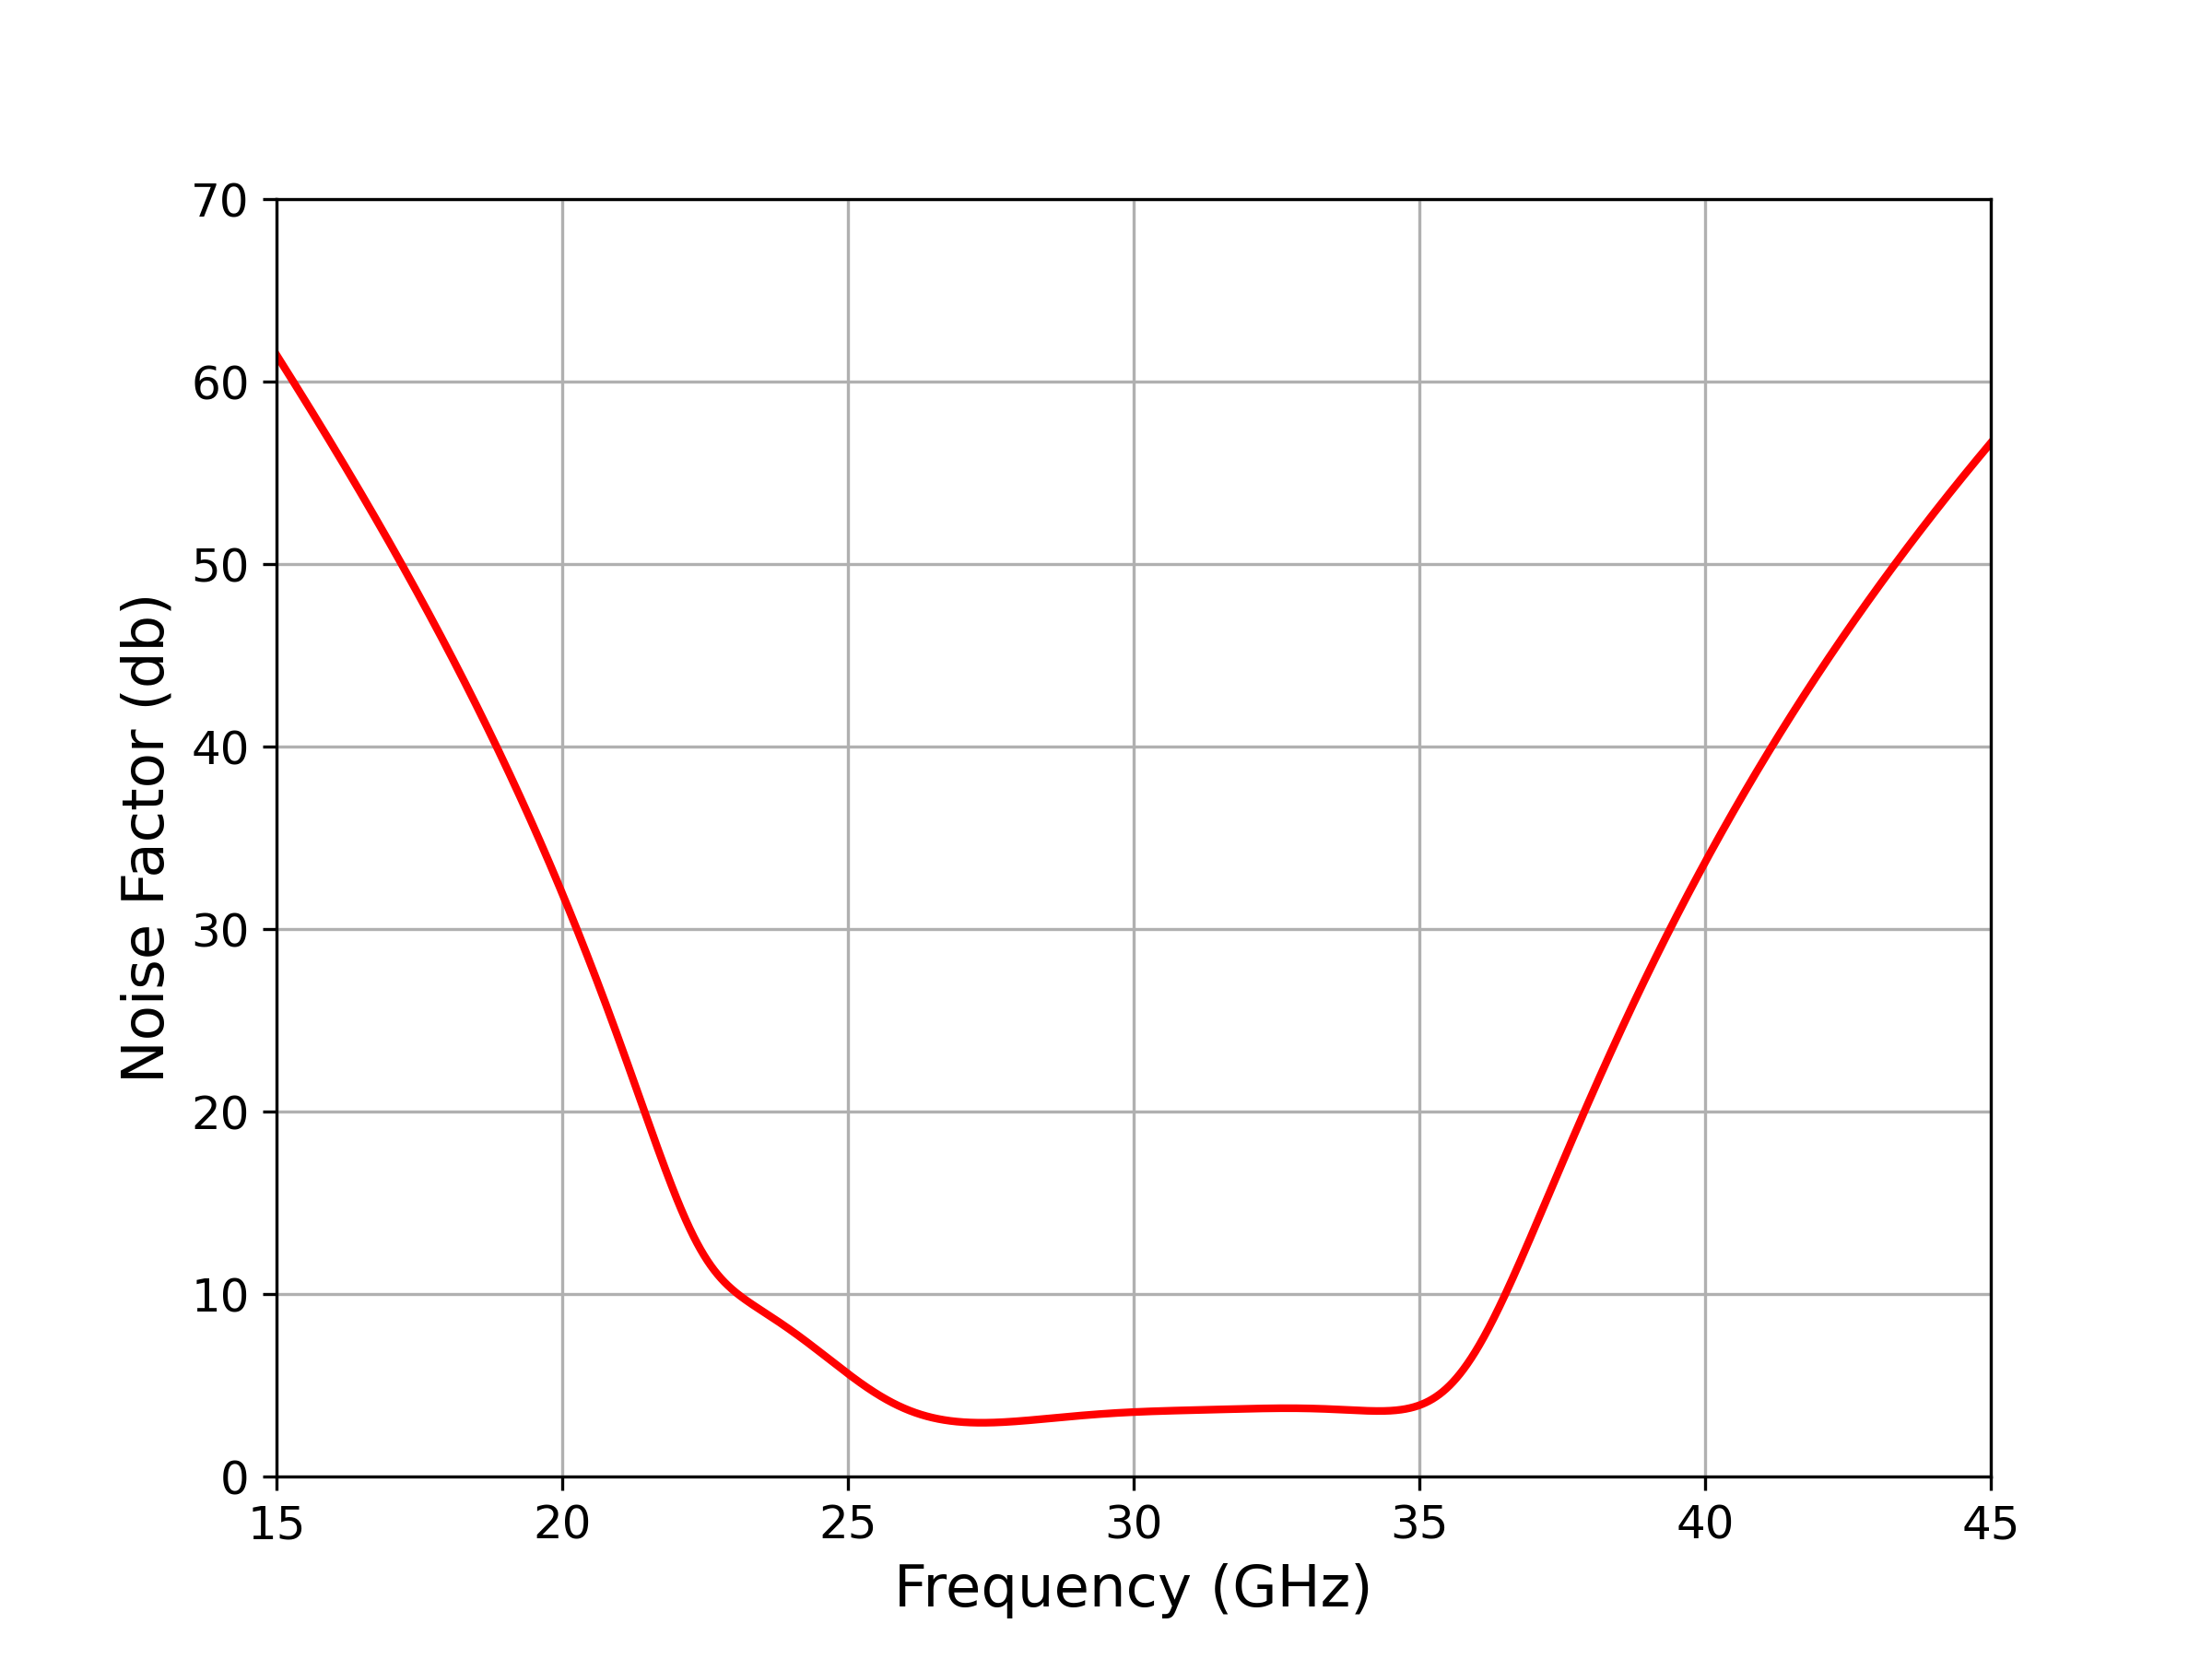
\includegraphics[]{figures/noise-factor.png}
%     }
%     \caption{Noise factor of a two-stage power amplifier (shown in Figure \ref{fig:two-stage-with-input-interstage-matching}) with input and interstage matching network.}
%     \label{fig:noise-figure}
% \end{figure}
% \begin{figure}[H]
%     \centering
%     \resizebox{0.8\textwidth}{!}{
%     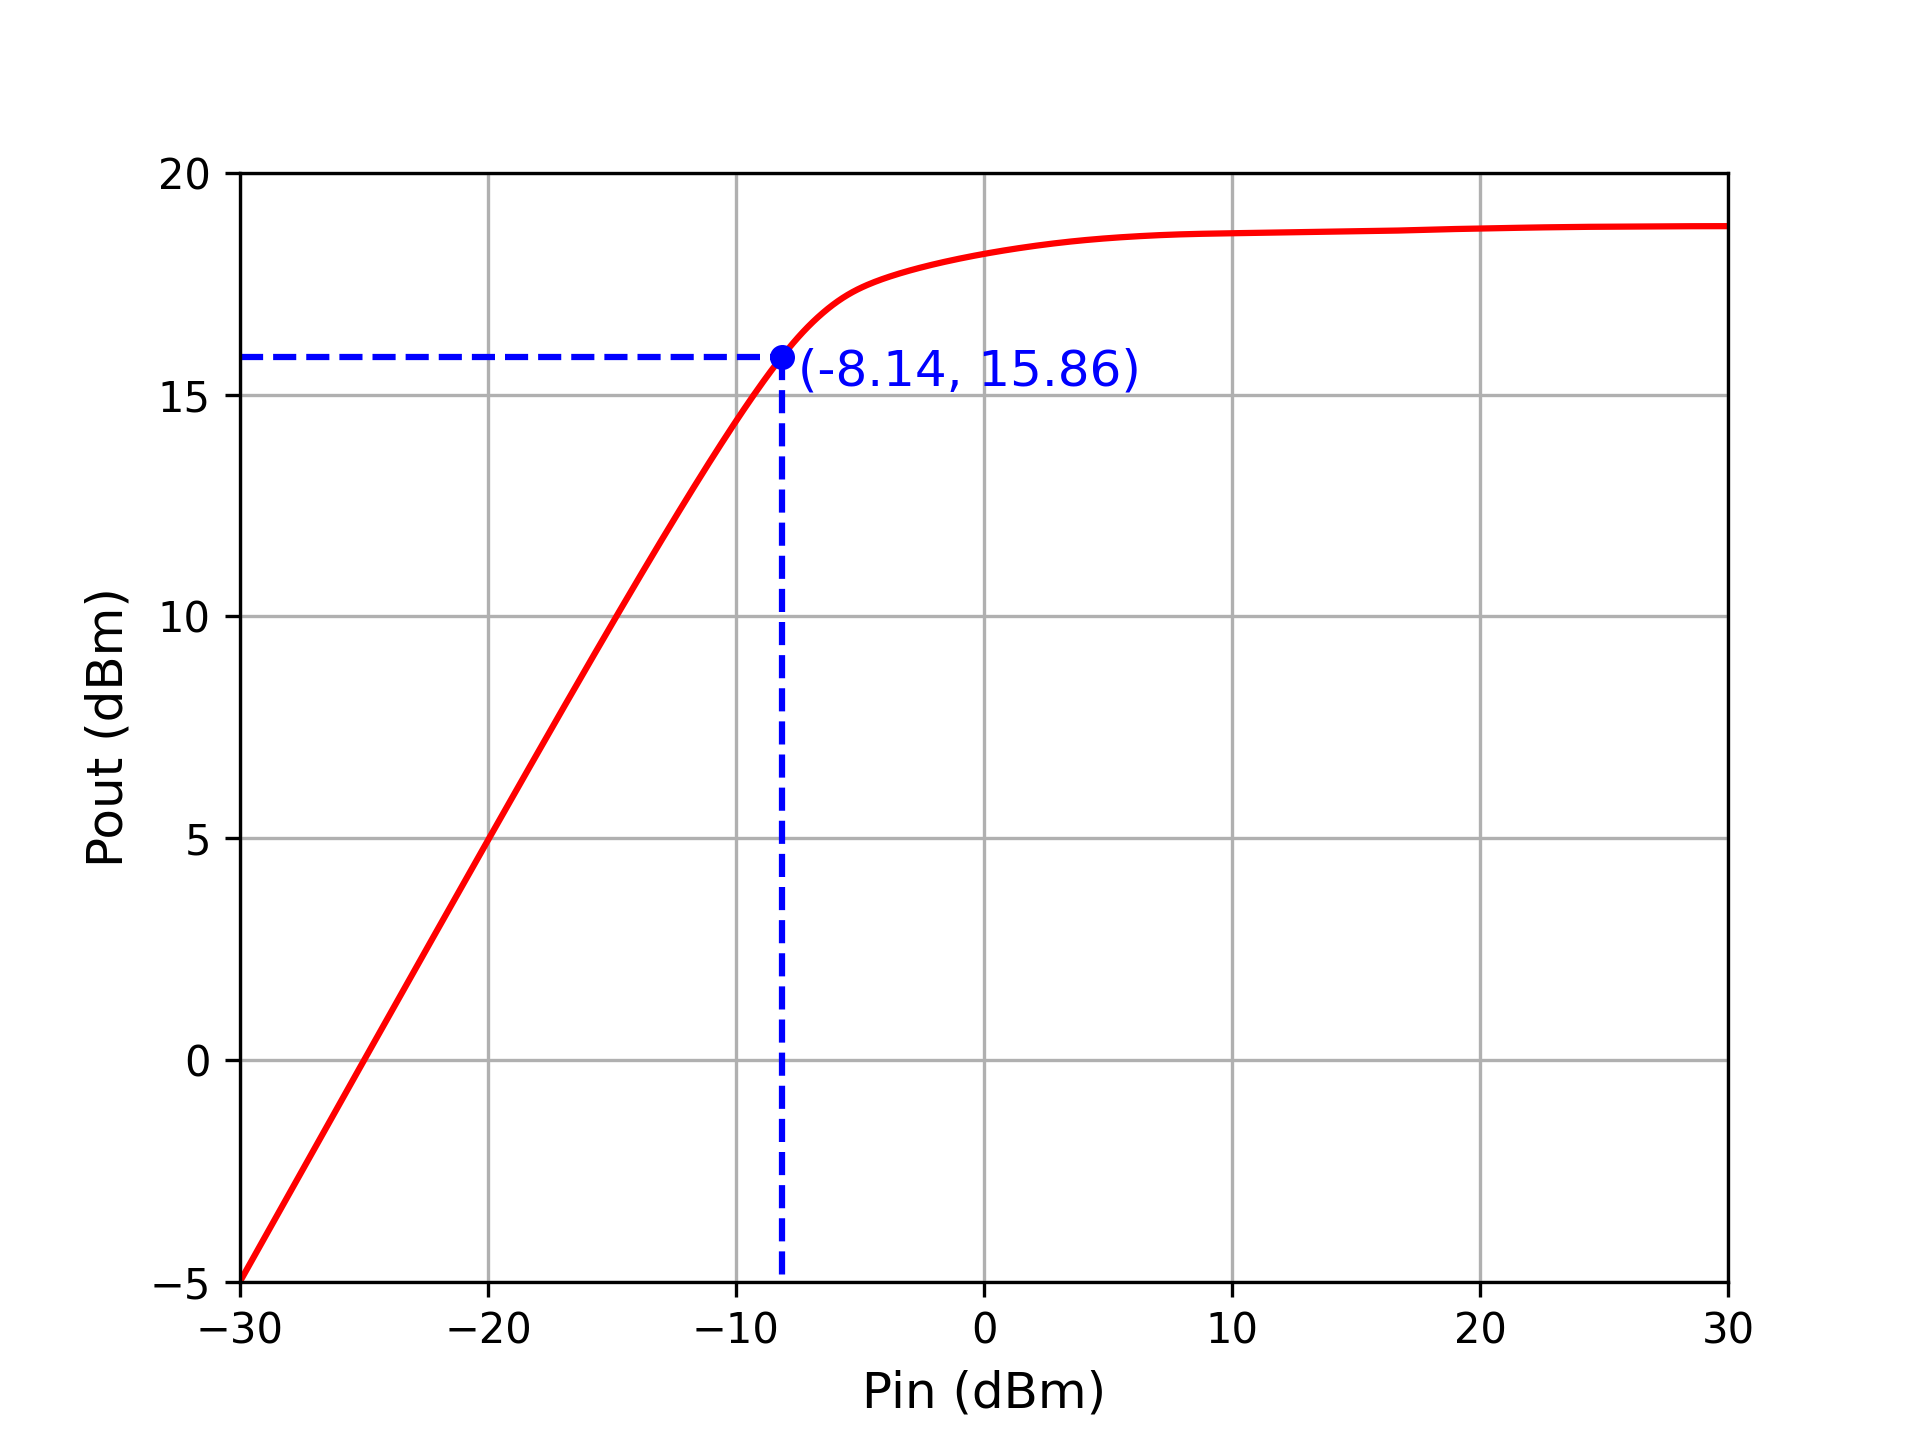
\includegraphics{figures/compressionCurves.png}
%     }
%     \caption{P1db compression curve of a two-stage power amplifier (shown in Figure \ref{fig:two-stage-with-input-interstage-matching}) with input and interstage matching network.}
%     \label{fig:compression}
% \end{figure}
\section{Analysis}
The given results describe the performance of a dual-band single-stage CMOS power amplifier circuit and its improvement through the addition of a second stage and matching networks. The key findings and implications of each stage and the matching network are given below.
\begin{enumerate}
\item Single-stage CMOS power amplifier:
The single stage CMOS power amplifier shown in Figure \ref{fig:single-stage-power-amplifier} and $S$ parameter simulation results $S_{11}$, $S_{12}$, $S_{21}$ and $S_{22}$ are shown in Figure \ref{fig:single-stage-without-cadence-s11}, \ref{fig:single-stage-without-cadence-s12}, \ref{fig:single-stage-without-cadence-s21} and \ref{fig:single-stage-without-cadence-s22} respectively.
    \begin{itemize}
       \item $S_{11}$: The value of $S_{11}$ at -0.17 dB indicates poor impedance matching at 18 GHz. This means that a significant portion of the power is being reflected back rather than absorbed by the amplifier, leading to inefficiency.
       \item $S_{21}$: The small value of 3.8 dB for $S_{21}$ indicates low power gain. This is primarily due to the parasitic capacitances and frequency-dependent transconductance of the CMOS transistors used in the amplifier circuit. These factors reduce the effective gain, especially at higher frequencies.
    \end{itemize}
\item Second stage addition:
The second stage was added using a staggered tuning technique to enhance gain and bandwidth.
The two stage CMOS power amplifier shown in Figure \ref{fig:double-stage-power-amplifier} and $S$ parameter simulation results $S_{11}$, $S_{12}$, $S_{21}$ and $S_{22}$ are shown in Figure \ref{fig:two-stage-without-cadence-s11}, \ref{fig:two-stage-without-cadence-s12}, \ref{fig:two-stage-without-cadence-s21} and \ref{fig:two-stage-without-cadence-s22} respectively.
    \begin{itemize}
        \item $S_{11}$: The value of -1.5 dB for $S_{11}$ suggests that input impedance matching has improved compared to the single-stage amplifier. However, further improvement may still be required.
        \item $S_{21}$: The power gain of 24 dB at 15 GHz indicates a significant enhancement compared to the single-stage amplifier. However, the gain decreases drastically as the frequency increases, which limits the bandwidth
    \end{itemize}

\item Matching network design:
    An input matching network and interstage matching network were designed using ADS (Advanced Design System) to improve impedance matching.
    The two stage dual band CMOS power amplifier shown in Figure \ref{fig:two-stage-with-input-interstage-matching} and $S$ parameter simulation results $S_{11}$, $S_{12}$, $S_{21}$ and $S_{22}$ are shown in Figure \ref{fig:two-stage-withmatching-cadence-s11}, \ref{fig:two-stage-withmatching-cadence-s12}, \ref{fig:two-stage-withmatching-cadence-s21} and \ref{fig:two-stage-withmatching-cadence-s22} respectively.
    \begin{itemize}
        \item $S_{11}$: The proposed PA network achieves better input matching with $S_{11}$ values of -16.38 dB at 27.12 GHz and -10.22 dB at 32.33 GHz. This indicates that a larger portion of the power is being absorbed by the amplifier rather than being reflected back.
        \item $S_{21}$: The maximum value of $S_{21}$ at 26.41 GHz is 27.55 dB, indicating a higher power gain compared to the previous stages.
        Average gain and gain at matching frequencies: The average gain across the frequency range of  25 to 35 GHz is 21.78 dB. At the matching frequencies of 27.12 GHz and 32.33 GHz, the gain values are 25 dB and 18.96 dB, respectively. These gains demonstrate the improvement achieved through the matching network.
        \item Output return loss ($S_{22}$): The proposed PA exhibits good reverse isolation with $S_{22}$ values of less than -5 dB, indicating that a small portion of the output power is reflected back.
        \item Reverse isolation ($S_{12}$) The proposed PA also exhibits good reverse isolation of -40 dB over the frequency range of 25 to 35 GHz.
    \end{itemize}
\end{enumerate}
Other important parameters:
\begin{enumerate}
\item 1 dB compression point (P1dB):
        The P1dB of the proposed PA is (-8.14 dBm, 15.86 dBm). This refers to the output power level at which the gain decreases by 1 dB from its constant value.
        Operating below the compression point is crucial to avoid non-linear behavior, distortion, and the generation of harmonics and intermodulation products.

\item $P_{sat}$:
        The $P_{sat}$ value of 12 dBm represents the maximum power level that the amplifier can handle without distortion.
        It is an important parameter for amplifier design and characterization.
\end{enumerate}
In summary, the initial single-stage CMOS power amplifier showed poor impedance matching and limited power gain. Through the addition of a second stage and the design of matching networks, improvements in input matching, power gain, bandwidth, and output return loss were achieved. The proposed PA demonstrated better performance in terms of gain, matching, and reverse isolation. However, it is important to operate the amplifier below its 1 dB compression point to avoid non-linear effects.
\newpage
\section{Performance Comparison Table}
\begin{table}[H]
  \centering
  \caption{Performance comparison with the wideband PA.}
  \label{tab:thesis_comparison_table}
  \begin{tabular}{|>{\centering\arraybackslash}m{1.5cm}|>{\centering\arraybackslash}m{1.5cm}|>{\centering\arraybackslash}m{1cm}|>{\centering\arraybackslash}m{1cm}|>{\centering\arraybackslash}m{1cm}|>{\centering\arraybackslash}m{1cm}|>{\centering\arraybackslash}m{2cm}|}
  \hline
  Ref. & CMOS Tech. & Gain (dB) & Freq (GHz) & $P_{1dB}$ (dBm) & $P_{sat}$ (dBm) & FBW (GHz) \\
  \hline
  This Work & 90 nm & 25 & 27.12 & 15.86 & 18.79 & (20.1\%) (25.66-31.1)\\
  \hline
  \cite{9829838} & 180 nm & 12.0 & 18 & 12.3 & 16.6 & (44.44\%) (14-22)\\
  \hline
  \cite{4729652} & 180 nm & 16.3 & 22 & 14.3 & 16.8 & (18.2\%) (20-24)\\
  \hline
  \cite{6634275} & 180 nm & 15.2 & 26 & 16 & 19.5 & (58.8\%) (18-33)\\
  \hline
  \cite{7890430} & 65 nm & 20.6 & 15.5 & 11.6 & 13.9 & (33.8\%) (13.5-19)\\
   \hline
   \cite{7742408} & 28 nm & 15.7 & 30 & 13.2 & 14 & (13.2\%) (27.4-32.2)\\
   \hline
   \cite{9252864} & 28 nm & 21.2 & 24 & 18.2 & 19.7 & (31.7\%) (21.8-30)\\
   \hline
  \end{tabular}
\end{table}
